\documentclass[12pt,twoside,openright]{memoir}

\usepackage[paperwidth=7in, paperheight=8.5in, inner=25mm, outer=15mm,top=20mm, bottom=20mm]{geometry}
\usepackage{fancyhdr}
\usepackage{color}
\usepackage{hyperref}
\usepackage{graphicx}
\usepackage{emoji}
\usepackage{tcolorbox}
\usepackage{listofitems}
\usepackage{fancyqr}

\graphicspath{ {./} }
\hypersetup{colorlinks=true, linkcolor=black, citecolor=black, filecolor=black, urlcolor=black}
\tcbuselibrary{skins,breakable}


\author{AmethystHeart2421}
\date{15 August 2022}
\setstocksize{8.5in}{7in}
\title{\textbf{\fontspec{Quantico}Engrams }\textbf{\small\fontspec{Open Sans} and } \textbf{\fontsize{1.5em}{1.8em}\selectfont\fontspec{Moon Dance}Moonwalks}}
\pretitle{\begin{center}\HUGE\bfseries}
\posttitle{\end{center}}


% SMS Colors
\definecolor{SMSFrom}{RGB}{18, 137, 254}
\definecolor{onSMSFrom}{RGB}{255, 255, 255}
\definecolor{SMSTo}{RGB}{229, 229, 234}
\definecolor{onSMSTo}{RGB}{21, 20, 26}
\definecolor{SMSTitleBack}{RGB}{246, 246, 246}
\definecolor{SMSTitleText}{RGB}{0, 0, 0}
\definecolor{DarkPurple}{RGB}{74, 38, 84}
\definecolor{LightPurple}{RGB}{105, 54, 120}

\setmainfont{Open Sans}

% setup human readible names for sms sfunciton
\newcommand\smsText{0}
\newcommand\smsFrom{1}
\newcommand\smsTo{2}

\makeatletter
\renewcommand{\maketitle}{%
	\thispagestyle{empty}% Remove page number on the title page
	\begin{center}
		\Huge\bfseries \@title\par
		\vskip 1.5em
		\Large \@author\par
		\vskip 1em
		\large \@date\par
	\end{center}
	\clearpage
	\@afterindentfalse\@afterheading% Reset indentation and heading
}

\newcommand*\cleartoleftpage{%
	\clearpage
	\ifodd\value{page}\hbox{}\newpage\fi
}

\newcommand{\tupleSwitch}[1]{
	\setsepchar{;}
	\readlist\mylist{#1}
	\foreachitem\tuple\in\mylist{
		\expandafter\tupleSwitch@i\tuple\relax
	}
}

\def\tupleSwitch@i#1,#2,#3\relax{%
	\ifcase#1
	% Case 0
	\textbf{#3}\newline \par
	\or
	% Case 1
	\smsFromBubble{#3} \par
	\or
	% Case 2
	\smsToBubble{#3} \par
	\else
	% Default case
	big~oof~FIXME!!!!!1 \par
	\fi
}
\newcommand{\dogPrintRule}{	
	\begin{center}
		\hspace{.5em}
		
\includegraphics[angle=60]{dogprint.pdf}
		\hspace{.5em}
		
\includegraphics[angle=120]{dogprint.pdf}
		\hspace{.5em}
		
\includegraphics[angle=60]{dogprint.pdf}
		\hspace{.5em}
		
\includegraphics[angle=120]{dogprint.pdf}
		\hspace{.5em}
		
\includegraphics[angle=60]{dogprint.pdf}
		\hspace{.5em}
		
\includegraphics[angle=120]{dogprint.pdf}
		\hspace{.5em}
	\end{center}
}

\newcommand{\pawsContinue}{
	
\includegraphics[height=0.8em]{dogprint.pdf}\hspace{.2em}
	
\includegraphics[height=0.6em]{dogprint.pdf}\hspace{.2em}
	
\includegraphics[height=0.4em]{dogprint.pdf}\hspace{.2em}
}

\newcommand{\nextMessage}{
	{\node[anchor=east, yshift=-0.5em] at (frame.south east) {
			\hfill
			\pawsContinue
		};
	}
}

\newcommand{\smsPic}[2]{
	\hspace*{0.2\textwidth}\includegraphics[width=0.6\textwidth, alt=#2]{#1}
}
\newlength{\myboxdifference}
\newlength{\smsboxwidth} %this seems wrong...

\newcommand{\smsFromBubble}[1] {
	
	\settowidth{\smsboxwidth}{#1}
	\ifdim\smsboxwidth>0.8\textwidth
		\setlength{\smsboxwidth}{0.8\textwidth}%
	\else
		\addtolength{\smsboxwidth}{3.4em}
	\fi

	\setlength{\myboxdifference}{\dimexpr\smsboxwidth-\textwidth\relax}
	
	\begin{flushright}
		\begin{tcolorbox}[halign=left, colframe=SMSFrom, colback=SMSFrom, width=\smsboxwidth]
			\raggedright\textcolor{onSMSFrom}{#1}
		\end{tcolorbox}
	\end{flushright}
}

\newcommand{\smsToBubble}[1] {
	
	\settowidth{\smsboxwidth}{#1}
	\ifdim\smsboxwidth>0.8\textwidth
		\setlength{\smsboxwidth}{0.8\textwidth}
	\else
		\addtolength{\smsboxwidth}{3.4em}
	\fi	
	\parbox{\smsboxwidth}{
	\begin{tcolorbox}[halign=left, colframe=SMSTo, colback=SMSTo, width=\smsboxwidth]
			\raggedright\textcolor{onSMSTo}{#1}
	\end{tcolorbox}
}
}

\newcommand{\smsConversation}[2]{
	\begin{tcolorbox}[
		breakable,
		title=#1,
		center title,
		colframe=SMSTitleBack,
		coltitle=SMSTitleText,
		colback=white,
		fonttitle=\bfseries,
		overlay unbroken=\nextMessage,
		overlay first and middle=\nextMessage
		]
		\tupleSwitch{#2}
	\end{tcolorbox}
}

\newcommand{\myQuote}[2]{
	#1
	\vspace{-1.25em}
	\begin{flushright}
		---#2
	\end{flushright}
	\vspace{.75em}
}

% Outline numbering
\setcounter{secnumdepth}{0}

\let\MyTitle\@title
\let\MyAuthor\@author
\let\MyDate\@date

%Redefine plain 
\fancypagestyle{plain}{%
	\fancyhf{}%
	\fancyfoot{} % clear all footer fields
	\fancyhead{} % clear all header fields
	\renewcommand{\headrulewidth}{0.0pt}%
	\renewcommand{\footrulewidth}{0.0pt}
}

\fancyhf{}
\fancyhead{} % clear all header fields
\fancyhead[RO]{\textbf{\MyTitle}}
\fancyhead[LE]{\textbf{\MyAuthor}}
\fancyfoot{} % clear all footer fields
\fancyfoot[RO]{\thepage}
\fancyfoot[LE]{\thepage}
\renewcommand{\headrulewidth}{0.4pt}
\renewcommand{\footrulewidth}{0.4pt}

\makeatother

\nonzeroparskip
\setlength{\parindent}{0pt}
\setlength{\parskip}{0.5em}

\begin{document}
\frontmatter

\pagestyle{empty}
\maketitle

\raggedright

\section*{}
\vspace*{\fill}
\begin{center}
For my husband, James, who gave me the idea to combine my obsessions with Scientology and Wolfstar. Also for patiently listening to me ramble on about this story for months. \emoji{face-blowing-a-kiss}
\end{center}
\vspace*{\fill}
\pagebreak
\section*{Acknowledgements}

This work was inspired by many fantastic Wolfstar authors, most especially MsKingBean89 and her work “All the Young Dudes” which brought me back to Wolfstar fandom after a 13 year break and inspired me to read more.

I was also inspired by Fantismal and Krethes and their amazing story, “Did You Miss Me?” for incorporating texting and images into a story to give it realism and depth.

I would be amiss not to mention Leah Remini for her series “Scientology and the Aftermath”, which helped me understand the experience of an ex-Scientologist.

And my friend Shannon, whose expertise on fashion shows was essential for this story! Thank you Shannon!

And of course, to my family for giving me the space and time I needed to write this story.

I couldn’t have done it without any one of you! \emoji{beating-heart}
\vspace*{\fill}\pagebreak
\section*{Kind words}
\myQuote{This is such an interesting premise! With Sirius getting pulled back in as Regulus gets sucked deeper into a cult! I really love how you are using the visuals of the app as part of the story!}{Katherington}

\myQuote{Omg, I just binged this fic in a day and absolutely loved it!!! You did a great job!!}{Whatever\_her\_name\_is}

\myQuote{So did I am I absolutely loved it, really delighted with how you ended it and the epilogue and happily ever after you gave them! \emoji{smiling-face-with-heart-eyes}\emoji{smiling-face-with-heart-eyes}\emoji{smiling-face-with-heart-eyes}\emoji{smiling-face-with-heart-eyes}}{YouBlitheringIdiot}

\myQuote{I really enjoyed this! What a nice ending for all these lovely characters.}{brandileigh2003}

\myQuote{Yay a happy ending for everybody! \emoji{smiling-face-with-hearts} This story was such a cool idea and you did amazing! \ldots\ Excited to read your other stories! \emoji{beaming-face-with-smiling-eyes}}{AstroKneazle}

\vspace*{\fill}
\pagebreak
\section*{Summary}
Modern Muggle AU taking place in the imaginary Southern California city of Hogsmeade.

The Black family are devout Scientologists, and Sirius has been disconnected from them for years. His religious trauma resurfaces when he finds a surprise from his brother, Regulus left on his front step.

Remus is a grad student studying to be a school psychologist. His mother is ill and his family is struggling financially. He decides to sign up to walk dogs at night for extra income. His first client is a male model living in the upscale neighborhood of Godric's Hollow. And neither of them can deny their attraction.
\vspace*{\fill}
\mainmatter
\raggedbottomsection

\pagestyle{fancy}
\chapter*{Chapter 1}
\textbf{Remus} 

``Are you getting enough to eat? You're so skinny! Do they even feed you at that school of yours?'' 

``No, Ma. They don't feed me.'' Remus sighed and sat in the cheap plastic chair next to the hospital bed. She's one to talk, he thought, bitterly. She was wasting away, barely recognizable as the strong, lively woman who raised him. Of course, it wasn't his mother he was angry with. Fate had just dealt her a shitty hand. It was frustrating, when the anger swirled inside him like this, that there was no one in particular that he could lash out at. 

``Well, what on earth are we paying them for, then? Someone needs to take care of my baby.'' Hope leaned over reaching out for his hand, which she grasped in both of hers. Her eyes were filled with concern. 

``Ma, I'm 23 years old. It's grad school. We pay them for the mediocre education that will get me a thankless job in a couple of years.'' In truth they weren't paying for school, exactly. At least not yet. There was no money for that. He had worked hard to earn scholarships that got him through his undergrad, and had some grants that helped pay for grad school, but he had still needed to take out student loans to cover most of the tuition, not to mention fees, books, and transportation. 

``What about that nice girl you were seeing? The one with the long red hair? I liked her.'' She smiled at him with a sparkle in her eyes that made his chest ache. 

``Lily. Yeah, she's great. But we're just friends, Ma.'' 

Hope wasn't discouraged at all, ``Yes, Lily. When I get out of this damn place, I'll teach her how to make all of your favorite meals. Someone needs to make sure you are eating!'' 

Remus just smiled and patted her hand. Lily actually really liked Hope and would probably happily submit herself to cooking lessons with her. But Remus doubted his mother would have the energy for it, even if she did recover enough to leave the hospital. At least, not any time soon.

At least she still sounded like herself. She sometimes got a bit confused or forgetful, which was to be expected with the toll the cancer, not to mention the treatment, was taking on her body. But she was definitely the same old Ma, worrying about taking care of him and not feeling sorry for herself for a single moment. His father, on the other hand, was a complete wreck whenever Hope fell ill. It was like he didn't know how to function in the world without her. 

As Remus was leaving the hospital, he was stopped by the front desk clerk. ``Mr.\ Lupin! Do you know when your father will be by again? There's been an issue with the insurance. I've tried to reach him all week but I only get voice mail.''

``Er, yeah, um, he's probably been busy. I'll talk to him about it. Thanks, Pomona.'' And dread dropped into his stomach like a stone. 

\dogPrintRule

``My mom asked about you yesterday. She wants to teach you how to make all of my favorite meals so you can fatten me up.''


Lily laughed as they inched up in the cafeteria line. He really enjoyed the days that he was doing his supervised field practice hours at Hogwarts High School and could get a fairly decent lunch for only a few dollars at the cafeteria. Plus, it was an opportunity to spend some time with his friend, who was a chemistry teacher there. They paid for their lunches and then headed outside toward the bench under the big shady willow tree, which had become their regular spot.
``I would actually love that! Her shepherd's pie is amazing, and my own mother was a shit cook. I have to look up videos on YouTube whenever I want to learn how to cook something.'' She shook her head, and they both focused on eating their lunch in companionable silence for a few minutes before Lily asked, ``So, how is Hope doing? She's been in St.\ Mungos for quite a while this time…'' Her voice trailed off as she fidgeted with the fork in her salad, eyes never leaving Remus's face. 

He looked up at her and smiled sadly. ``She's okay. I mean, not well enough to leave the hospital any time soon, but she seems in pretty good spirits at least. I'm going to see her again Sunday morning, if you want to join me. I know she'd love that.''

``Yes, of course!'' Lily answered quickly. ``That would be wonderful. And I'm taking you out for breakfast first. I won't have your mother accusing me of letting you waste away. I'm not taking no for an answer, Remus Lupin!'' 

``Well, I guess you leave me no choice.'' He beamed gratefully at his friend as he took another big bite of his sandwich. 

\dogPrintRule

\textbf{Sirius} 

``Great shoot, as always, Black!''

``Couldn't have done it without you, McKinnon!'' Sirius grinned and draped an arm over Marlene's shoulders as she held up her camera so that he could see the view screen. They looked through the images from the photo shoot making notes of the ones with the best lighting, or those that would need more editing, and laughing at the obvious throw-away shots. 

``Don't even think about leaving with all of that make-up on, Black. I need you back here for a good scrub down.'' Mary, his make-up artist, called out, clearly anxious to finish up for the day.

``Yeah, yeah, I'm coming, Macdonald. Keep your pants on.'' He reluctantly backed away from Marlene, continuing to comment on the images she was scrolling through until his view was blocked as he took his seat in the makeup chair. 

Mary handed him a bottle of water and got to work on his face. ``So, the old gang is going out to The Three Broomsticks tonight. Think you will be gracing us with your presence?'' she asked.

``The Broomsticks? Isn't that place right by the university? It'll be crawling with college students.'' Sirius was terrible at coming up with excuses, but he really just wanted to go home and binge watch whatever crappy superhero show was currently trending on Netflix, avoiding humans altogether. 

Mary scoffed, ``Exactly! Sirius, you need to get out and have some fun. How are you going to meet people moping around your mansion all the time? A fresh young college student could do you some good.'' 

``Hey, I meet people around the mansion! The new night guard at Godric's Hollow, Shacklebolt, he's a great guy. We have fascinating talks. You know he trains wild animals as a hobby? The guy has a pet lynx!'' 

Mary stared at him for a few beats before she busted up, laughing, ``Sirius Black, you are coming out with us tonight. Go home and put on those tight black jeans that really show off that ass, and we'll pick you up at nine.'' 

Sirius sighed, resigned. ``Okay, okay. But I'm bringing Prongs, I need a reliable wing-man.'' 

Mary did a little dance of joy, and hugged him from behind, talking to him in the mirror. ``Yeeeaaah! We're gonna have so much fun! Just like the old days.'' 

``Can't wait.'' 

\dogPrintRule

The pub was indeed crowded, and noisy, but Mary was right; it was great to be out with the old gang. Along with Mary, Marlene, and her girlfriend, Dorcas, they were joined by Gideon and Fabian Prewett, models and actors who had been much more successful than Sirius in building public recognition. He was secretly grateful, as their presence meant they chose a large table nestled in the corner of the pub to try to minimize exposure. And most of the attention they did get from strangers was directed at the red-headed twins. 

``Is Emma going to make it? Haven't seen her in ages.'' Fabian asked as he returned to his seat after posing for a selfie with a couple of giggly college girls. Gid passed him a fresh pint of lager, which he accepted gratefully, taking a long swig. 

``Nope, she's on tour as a backup dancer for The Weird Sisters, didn't you know?'' Mary yelled over the din of the bar.
``Honestly Fab, keep up! She's been posting about it on Insta all week! I'm so jealous, you all have such glamorous lifestyles.'' She put on a posh accent and lifted her apple martini with her pinky finger sticking out, and Dorcas snorted a laugh beside her. 

Sirius rolled his eyes and leaned back ``Your life is plenty glamorous. You get to practice your art on this incredible canvas!'' he stuck out his chin and haughtily brushed his hair back from his face, sending Mary and Dorcas into a real fit of giggles. 

James just shook his head smiling at his friends as he took a sip of his beer, addressing Gideon as he set it down. ``Hey Gid, how's Molly doing? I heard she had another baby recently?'' 

``Yup! Another boy! I know Mols was secretly hoping for a girl, so I honestly don't think they're done yet. Oh, let me show you some pictures!'' And he pulled out his phone, every bit the proud uncle, and leaned over to show James and Sirius as he swiped through pictures of two red-headed toddler boys and a pink little chubby newborn. ``That's my favorite there, little Billy holding baby Percy for the first time!'' 

``Oh, Gid, they're adorable!'' Mary purred as the phone got passed around for everyone to gush over. 

Maybe it was the beer, he was a few pints in, but Sirius felt a rush of affection for his friends. They had all met at the private Performing Arts high school that he started attending when he was 14. His parents had seen his natural charm and conventionally handsome features as their possible ticket to celebrity. In their religion, that was basically like a calling to the priesthood. Celebrities have unparalleled power and influence which they can use to help ``clear the planet''. And so they poured money into getting Sirius into a prestigious modeling program and hiring a prominent agent, and working to get invites to events in which he could work his charm on the rich and the famous. Unfortunately for them, their plan backfired. For the first time, Sirius made real friendships with people outside the church, which is what slowly started putting cracks in his faith. 

Mary nudged Sirius and whispered ``That guy over there has been checking you out for the last ten minutes.'' She nodded toward a very handsome young man a few tables away. He had wavy blond hair and startling blue eyes, and when Sirius glanced over at him he broke into a grin showing off a set of perfect, white teeth. Sirius put on the smile he had learned to use when trying to impress people, it was just an automatic response by now. He grumbled to Mary, ``Oh Mare, look what you've done, now he's coming over!''

``Good!'' Mary snickered. ``Oh, look, I suddenly need a new drink.'' And she stood up, offering her seat to the blonde man who had just arrived.

His name was Gilderoy, which Sirius thought was a ridiculous name, but he was very good looking. So Sirius turned on the charm, smiling and making smalltalk. Which, with Gilderoy, was mostly listening to him talk about himself and all of his amazing accomplishments. When he did start asking questions, it seemed unnatural and forced, and there was something about the words he used, the way he asked about Sirius's family and about his Instagram following, that made anxiety start to crawl up Sirius's spine. He looked over at James, and that was all he needed to do. James had sent a message to their driver, made an excuse to their friends, quickly gave hugs, and pulled Sirius out the door, all within minutes.

\chapter*{Chapter 2}

\textbf{Remus} 

``More coffee for you sweetheart?'' 

``Yes, please!'' Remus answered the waitress, a pretty, petite blonde named Flo, according to her name tag. She had a lilting southern accent, which made the pet name sound endearing rather than obnoxious. She refilled their coffee and rushed off to the next table amid the Saturday morning breakfast rush.

``So, it looks like I'll have to change my phone number again.'' Lily sounded resigned as she held her mug with both hands breathing in the aroma.

``Oh no. Not Snape again? What happened?'' Remus asked, setting down his own mug and pushing aside the menu he'd been salivating over while trying to decide what to order.

``I started getting messages last week. I blocked the number, but yesterday it started again from yet another unknown number.'' She pulled out her phone and tapped it a few times to pull up the messages, passing the phone to Remus to see them.

\pagebreak
\vspace*{\fill}
\textbf{12:40pm}
\smsConversation{Unknown Number}{
	\smsFrom, {Snape}, {Lily, I know you are getting these messages. Look, we obviously have had some miscommunication. I just want to talk. Whatever Mulciber told you was a lie. I would never say anything bad about you. Our friendship is too important to me. -Severus};
	\smsFrom, {Snape}, {Please let me know when we can talk. You can reach me at this number. -Severus};
	\smsText, , {Missed call from Unknown Number 7:03pm};
	\smsText, , {Missed call from Unknown Number 7:50pm}
}

\pagebreak
\vspace*{\fill}
\textbf{8:30pm}
\smsConversation{Unknown Number}{
	\smsFrom, {Snape}, {Lily, I'm worried about you, I need you to answer my calls. Avoiding speaking to me is not going to resolve anything. I'm starting to get angry.};
	\smsText, ,{**number blocked**}
}

``Jesus, Lils. This guy is such a creep! How do you think he got your number?'' Remus handed back the phone with a slight shudder. Lily had been dealing with Severus's obsessive behavior for over a year now. They had been in a tutoring group together in college and they were actually friends. Not like ‘hang out at the bar' or ‘watch movies at each other's houses' friends, but ‘text each other about homework' and ‘offer rides to class' kind of friends. 

During their last semester before graduation, he asked Lily out on a date and she declined. She was very kind about it, insisting that she valued his friendship, but she just wasn't interested in him in that way. That's when things got a bit out of hand. He would write threatening notes to other men that she went out with. He even followed Remus around sometimes sneering at him and accusing him of doing inappropriate things with Lily and turning her against him. Their friends Alice and Frank woke up one day to find their mailbox smashed and rude words spray painted on their garage door.

After graduation, Lily got a new apartment close to her new job at Hogwarts, and changed her phone number. Things seemed quiet for a few months. Remus had hoped she was in the clear now, and that Severus had moved on to some other attractive girl to terrorize. Apparently that was not the case.

``I don't know. But I don't think just blocking him again will do much good. He'll just use a different number. I really don't know what else to do. Maybe if I change my number again, he'll finally give up?'' she said this hopefully, but he could hear the doubt and fear in her voice. Remus reached across the table to hold her hand in sympathy. He was at a loss for how to help her. And then Flo was back to take their order. They both ordered waffles with eggs and bacon, and tried, for the moment, to drown their problems in maple syrup.

\dogPrintRule

Before leaving St.\ Mungos, Remus was stopped by the front desk clerk, Pomona, again. She filled him in on the situation, since his father had not yet resolved it. The insurance had denied the claim for one of the medications that his mother was on, leaving them with a rather large bill. He assured her that he would take care of it, but he would need time. He really didn't want to tell his father about this new debt being added to the already insurmountable pile. Remus decided right then that he would find a way to help pay off the debt. But it wasn't going to be easy. Between grad school courses, field experience hours, and visits to his mother, he really didn't have a lot of time for a job.

``I'll have to find something part time in the evenings. But it will have to be pretty flexible.'' He told Lily as they left the hospital and he grabbed a newspaper from a news stand and started looking through the pages for the classifieds.

``If you had a car you could do one of those ride share services. You know where you just pick up rides whenever you have the time and make extra money that way.'' Lily said, rather unhelpfully.

``Maybe I could get a bicycle and do deliveries around Hogsmeade. Like picking up fast food for drunk college students or something.'' Remus suggested, thinking maybe they were actually on to something.

Just then he crashed headlong into another man coming around the corner. The man had four dogs on leashes, which was obviously a bit much for him to handle, and two of the dogs were now chasing each other around Lily and Remus effectively tying them up like burglars in an old-timey cartoon. The man spluttered apologies as he worked to wrangle the dogs and Remus and Lily barely kept from falling over as they untangled themselves from the mess.

``I'm so sorry about this! Maybe four dogs is one too many. I'm Davey, by the way.'' He smiled apologetically at Remus and put out his hand to shake, but his arm was quickly jerked away by a dog who's leash was attached to it.

``Are these all your dogs?'' Remus laughed as a golden retriever jumped up to lick his face with its big pink tongue, and he happily scratched it behind the ears. Remus had always loved dogs. His family never had them, because his dad was allergic. But as a kid he would spend hours at friends' houses playing with their dogs. His ex-boyfriend, Benjy, had had a German Shepherd named Bertha that he adored. He's pretty sure he stayed in that relationship too long because he couldn't bear to say goodbye to Bertha.

``Oh, no, they're not mine.'' Davey responded. He finally seemed to have control over the three dogs that weren't currently being petted by Remus. ``I'm a dog walker. Ever heard of ‘Bark to the Park'? It's an app kind of like Uber, but for hiring someone to walk your dog.'' 

Lily gasped and grabbed Remus's arm, an open mouthed grin spread across her face. She was thinking exactly what he was thinking. Dog walking, of course! That's something people get paid to do, and it's part time, and dog walkers can probably make their own schedules. It was perfect. ``I haven't, but I would love to hear more.'' 

\dogPrintRule

\textbf{Sirius} 

``Thanks again for having my back last night.'' Sirius said as he wiped sweat from his brow. He and James were in their private gym getting in a nice morning workout. James was huffing away on the treadmill. He hit some buttons to slow it down so he could respond.

``You really think that guy was a spy for the church? Maybe he was just really bad at flirting.'' he managed to get out, while his heart rate slowed to a more reasonable pace for holding conversation.

``I just got that vibe from him, Prongs.'' Sirius said a bit defensively, as he stretched his aching muscles. ``I'm not being paranoid.''

``No, I know, I know. You're usually right about these things. Maybe you should try one of those dating apps to meet people. Better chance to vet them before meeting in person, you know?''

``Better chance for those creeps to find me, you mean.'' Sirius's stomach churned. He hadn't really dated anyone since High School. Maybe he was paranoid, but he felt like everyone who showed an interest in him had ulterior motives. He just couldn't shake the feeling that the church still had people watching him. Following him whenever he was out in public. It was just easier to stay in. Safer. Better this way.

The doorbell rang out the chorus of ``Jingle Bells'', and Sirius groaned. ``Prongs, Christmas was months ago, can we change the damn door bell already?''

``I like it, it's cheery!'' James grinned at him. 

The doorbell jingled again. Sirius grabbed his water bottle, taking a long swig. ``Isn't someone going to get that? Is Winky here today?''

``Nope, she has Saturdays off now. Her kid's in a soccer league.'' James hit some buttons to increase the speed on the treadmill again, clearly not willing to stop his workout to answer the door.

``Alright, alright, I'll get it.'' Sirius wrapped his towel around his neck and jogged up the stairs to head to the front door. He didn't see anyone through the peephole, so he opened the door to check for a package. Something had been left on the front step, but it wasn't from UPS. It was a small black and brown dog, with a leash tied to a carrier. The dog whined and tried to pull away from the carrier. Sirius noticed a note attached to its collar. He picked up the squirming animal and pulled the note off to read it quickly.

\textit{Sirius,} 

\textit{I have signed a billion-year contract. I know you won't approve, but I really believe this is the best way for me to do my part to help clear the planet. }

\textit{This is Barty. He's 2 years old, and his papers and medical records are in a binder in the carrier. I also left some of his favorite toys and enough food for a few days. I told mother I was dropping him off at the shelter, but I just couldn't do that. I feel better knowing he is with you. Please take good care of him for me. }

\textit{When you are ready to do the right thing, I still have hope that I will see you (and Barty) again.} 

\textit{Your Brother,\newline R.A.B.} 

Panic flooded through Sirius as he set down the dog and ran down the walkway, looking frantically in every direction.
``Reg!'' he called out, desperately, ``Regulus!'' but he didn't see anyone. Damn it, why had he waited so long to answer the door! He could have stopped him! He could have talked some sense into him! He ran to the property gate, but there was no guard posted there, so someone would have had to buzz him in, or else he had managed to follow in another neighborhood resident. He looked up and down the empty street and cursed. 

He slowly trudged back up the walk to where Barty was choking himself in an attempt to escape the leash. Sirius sighed, resigned, picked up the dog and brought him into the house.

\chapter*{Chapter 3}

\textbf{Remus} 

Remus had exchanged numbers with Davey, helped him get his furry clients under control, and promised to be in touch. Davey had given him some great advice about setting up an account with ``Bark to the Park''. First, he had to fill out an application, including references about how good he was with dogs. He hoped Benjy wouldn't mind putting in a good word for him. They had ended on amicable terms, but really hadn't spoken much since they broke up. Maybe he should call him and ask before putting him down as a reference? He should probably take him to coffee to thank him, too. The thought made his stomach flip and Remus suddenly felt very lonely. He stamped down the urge to call and instead just sent a quick text message as a heads up.

Next, was setting up a profile. You could choose a profile name and add a short bio to let people know your preferences and availability. For example, if you preferred small dogs or big dogs, short walks or long walks, etc. Remus knew he was only going to be available at night, which probably wasn't the most in demand time for dog walkers. But he hoped he could pick up enough jobs here and there for people who just needed a night off, or went on business trips and didn't want to hire a dog sitter. He uploaded a picture for his profile that Alice had taken last year and he was quite fond of. It only showed the right side of his face, so you couldn't see the ugly scar that stretched from a couple of inches in front of his left ear to past his hairline. He was smiling in the picture, laughing at something Frank had said, and he thought it helped him look friendly and trustworthy. 

So that was that. Now he just needed to wait for his background check to be approved and he could start booking jobs. It felt good to be doing something, anything, that could relieve the pressure on his family, and the knot of dread in his stomach seemed to loosen just a little.

\dogPrintRule

\textbf{Sirius} 

Sirius barely left his bedroom for the next couple of weeks. He completely ignored his furry little problem, allowing him to wreak havoc throughout the house. He could hear Winky complaining about it to James, and James apologizing and making excuses and running around trying to clean up Barty's messes before the housekeeper saw them.

There was a soft knock at the door. ``Go away.'' Sirius growled. 

``Come on, Pads. I know you're upset, but you can't just hide in there forever. At least let me come in so we can talk?''
God, why did he have to be so kind and understanding all the time. It made it impossible to yell at him when all he wanted to do was yell, or cry, or just disappear all together. 

``Ugh, fine, come in.''

James cringed a little at the state of Sirius's room, but he didn't say anything about it. He just came over to his bed and sat at the edge. ``So, do you want to talk about it?'' he asked, and watched Sirius patiently, waiting for a response.

``Not really.'' He didn't know if James meant Barty or Regulus. Either way, Sirius wasn't sure he was ready to face it. Regulus's note had sent him right back into a depressive spiral, similar to when he was 16 years old and first disconnected from his family. The Potters had taken him in then, and he had never left. He had relapsed a few times over the years, and James had always been there for him. He seemed to know that the best thing to do was let Sirius be alone for a while and then slowly try to bring him out of it, when he was ready. 

This time had been really rough though. Regulus had joined the Sea Org. He had held on to hope that his brother would come to him one day and say that he had had enough of their cultish religion and he wanted out. And Sirius would help him set up a new life, away from their family and everyone connected with the church. And they could be brothers again. It was stupid, but he had really believed it would happen. And now that dream was shattered. He had lost him for good.

``Do you want me to call Dr.\ Pomfrey?'' James suggested. The psychiatrist specialized in helping people coming out of extremist religions, but his case was particularly difficult since it came with an excessive distrust of psychiatrists and psychologists in general. But Dr.\ Pomfrey would prescribe medications, no questions asked, which was sometimes a help. Sirius considered it. 

``Maybe.'' he mumbled, playing with the bedsheet. 

``Okay great, why don't you get in the shower and I'll give her a call. Then meet me in the kitchen and I'll make you a smoothie and we will talk about how to deal with this dog situation.'' James said cheerily, as though everything was better now. 

``Okay, okay. I'm moving.'' Sirius dragged himself out of bed. ``But I want real ice cream, not your stupid protein powder crap!'' he called back as he entered the bathroom and James laughed.

\dogPrintRule

``He probably just needs to get some of his energy out. I can take him out in the mornings for a jog before I go to the office.'' James offered as he handed Sirius his smoothie. James had inherited a majority share of his parent's company when they died, and made enough passive income that he really didn't need to work at all. But he had gotten a degree in Corporate Law and actually enjoyed his work. Still, Sirius thought, it had to be weird working in an office with people who knew you were technically the owner of the company. James was so friendly and carefree though, it didn't seem to affect him at all. ``You're going to have to take him out at night though, wear him out enough that he doesn't tear the place up while we're sleeping.''

Sirius made a face as he sipped his smoothie, which was definitely not made with ice cream. ``I could just hire someone to do it.''

James glared at him. ``Really, Padfoot, it's not like the fresh air wouldn't do you some good too, you know.''

``I could be busy at night. Marlene and Dorcas have been trying to get me to go out more often.'' Sirius retorted stubbornly.

``Oh, you're suddenly Mr.\ Night-On-The-Town now?'' James scoffed.

``Yeah, you know me.'' Sirius pulled out his phone and started tapping the screen. ``Oh look! Here's an app where you can hire a dog walker!'' He waved the phone. James shook his head and sat down next to him, sipping his own smoothie.

Sirius was scrolling through the list of dog walkers in the area, grimacing as he inadvertently took another sip of the smoothie. Then his face brightened suddenly. ``Ooh, here's a good one! He's a grad student, available for evening walks. Mmm, he's cute too. Wonder if he's single.'' he wiggled his eyebrows at James, smirking. An odd little thrill went through him as he read the user profile for \textit{MoonWalker06}. He really did need to get out more.

``Well, you certainly seem back to your old self.'' James said with a note of relief. ``Just remember that's not a dating app.'' he chided, pointing at Sirius's phone.\newline
Sirius winked at his friend.. ``Sure, sure. I want this one!'' and he tapped the button to send a message.


{\hfill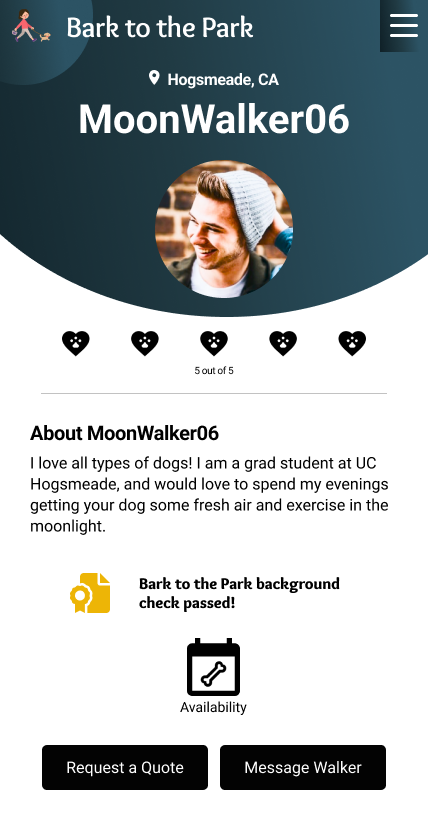
\includegraphics[height=\textheight]{profile}\hfill}
	

\chapter*{Chapter 4}
\textbf{4:30PM}\nopagebreak
\smsConversation{Bark to the Park}{
	\smsFrom, {Bark to the Park}, {You have a message from Bark to the Park user, Padfoot12.};
	\smsFrom, {Bark to the Park}, {Type Yes to accept the message};
	\smsTo, {MoonWalker06}, {Yes}
}

\smsConversation{Padfoot12}{
	\smsFrom, {Padfoot12}, {Hello, MoonWalker06. I would like to request your services for an obnoxious miniature pinscher that needs walking. Does 8:00 work for you? Which days are you available?};
	\smsTo, {MoonWalker06}, {Hi, that's great, I'm sure they are nothing I can't handle. \emoji{winking-face} Right now I am available every evening except for Wednesdays and Fridays.};
	\smsFrom, {Padfoot12}, {Okay cool, let's book an hour on all of those nights. Do you know where Godric's Hollow is?};
	\smsTo, {MoonWalker06}, {Yup, no problem! So, five nights a week? The app has my rates, just want to make sure that is okay with you.};
	\smsFrom, {Padfoot12}, {Of course, but I do have one very important question before we proceed.};
	\smsFrom, {Padfoot12}, {Can you really moonwalk?};
	\smsTo, {MoonWalker06}, {Oh, haha, the username. I just thought it was a clever way to indicate I am only available for night time walks.};
	\smsFrom, {Padfoot12}, {That doesn't really answer the question, Moonboy \emoji{winking-face-with-tongue}};
	\smsTo, {MoonWalker06}, {Well, yes, I can moonwalk. I mean, it's not that hard. Can't everyone?};
	\smsTo, {MoonWalker06}, {I look forward to meeting Padfoot (I assume that's your dog's name?) Did you want to start tonight?};
	\smsFrom, {Padfoot12}, {Ah, haha no the dog is called Barty. I'm Padfoot.};
	\smsFrom, {Padfoot12}, {I mean yes. About starting tonight. Barty looks forward to meeting you, too. \emoji{smiling-face-with-smiling-eyes}};
	\smsTo, {MoonWalker06}, {Barty, that's an interesting name for a dog. Short for Bartholemew?};
	\smsTo, {MoonWalker06}, {Padfoot is an interesting name for a human.};
	\smsFrom, {Padfoot12}, {It's short for Bartemius actually. It's a stupid name for a dog. My weird brother named him.};
	\smsFrom, {Padfoot12}, {Padfoot is a perfectly normal name for a human, Moony. (*\string^{\fontspec{Inter}\symbol{"203F}}\string^*)}
}

\textbf{8:00PM}\nopagebreak
\smsConversation{Padfoot}{
	\smsTo, {Moony}, {Hi, I am at the gate at Godric's Hollow and I realize now I should have asked for more information. There is no button here labeled ``Padfoot'' or ``Bartemius''};
	\smsFrom, {Padfoot}, {Oh, shit, right. Sorry, Moony --- Just give me a minute. I'll send someone out with him.};
	\smsTo, {Moony}, {No problem. So, I guess my name is Moony now?};
	\smsTo, {Moony}, {Okay, I have Barty};
	\smsTo, {Moony}, {I met your night guard. Nice guy. Did you know he has a pet lynx?? I didn't even realize that was legal.};
	\smsTo, {Moony}, {\smsPic{taylor-heery-tOsfvWC\_fFo-unsplash (1)}{}};
	\smsTo, {Moony}, {As much as I like my new name, you are entitled to know my actual name now that I have your dog in my possession and everything. If you are interested.}
}

\textbf{8:10PM}\nopagebreak
\smsConversation{Padfoot}{
	\smsFrom, {Padfoot}, {I would love to know your name, Moony.};
	\smsFrom, {Padfoot}, {I also want to know where you got the socks. Those are amazing.};
	\smsFrom, {Padfoot}, {And he's not really my dog. I'm just looking after him for a while. With your help, of course. \emoji{winking-face}};
	\smsTo, {Moony}, {I'm not sure where I got them. I just pick up interesting socks when I see them. I'm not going to do my moon-walking in boring socks, am I? I mean, that would be weird. \emoji{winking-face-with-tongue}};
	\smsTo, {Moony}, {Remus, by the way. My name is Remus.};
	\smsFrom, {Padfoot}, {I admire your dedication to originality, Remus.};
	\smsFrom, {Padfoot}, {BTW, I noticed that the app has a feature that can notify owners of every time their dog takes a shit or piss. I expect to be notified of all of Barty's bodily excretions.}	
}

{\hfill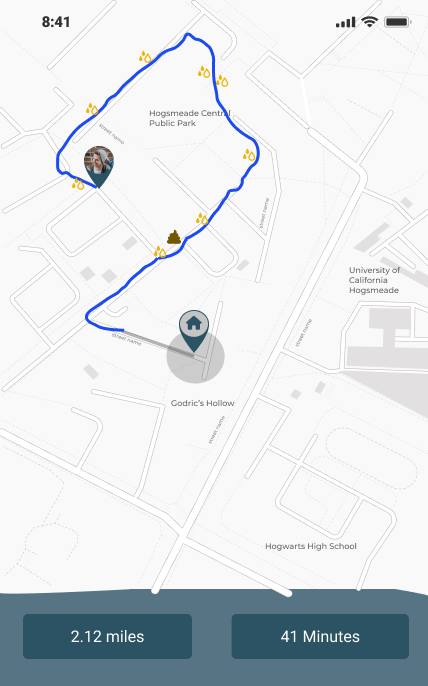
\includegraphics[height=\textheight]{iPhone 13 Pro Max - 3}\hfill}

\textbf{8:50PM}\nopagebreak
\smsConversation{Padfoot}{
	\smsFrom, {Padfoot}, {That's a lot of bodily excretions.};
	\smsTo, {Moony}, {It's dark out. It's hard to tell if anything is actually coming out, so I figured I'd just let you know every time he lifts his leg by a bush or a rock or a mailbox, etc, etc. It could be important information for a dedicated pet owner such as yourself.};
	\smsFrom, {Padfoot}, {Good call. Thanks, Moony.};
	\smsTo, {Moony}, {Just doing my duty, Padfoot.};
	\smsFrom, {Padfoot}, {If you are expecting a ``doody'' joke, then you can just forget it. I am too mature for that, Moony.};
	\smsFrom, {Padfoot}, {Thank you for your excellent work tonight. Barty is as happy and relaxed as I've ever seen him. He looks forward to seeing you tomorrow night.};
	\smsTo, {Moony}, {Barty was a pleasure to walk with, Padfoot. You can tell him I look forward to seeing him, too. Good night.}
}

\chapter*{Chapter 5}

\textbf{Remus}


``You are all smiles today, Remus! What's going on? Is there a new beau in your life?'' Lily raised her eyebrows teasingly. They had just sat down with their lunches in their shady spot under the willow tree.

``Haha. No. But I got my first regular client from Bark to the Park. You know Godric's Hollow?'' he said as he tore open a ketchup packet, squeezing it over his fries.

``Yes. Oh my god! Are you a dog walker for the rich and the famous now?'' She shrieked, grabbing his arm in excitement.

``Something like that? I'm not sure who the owner is. The guard called him Mr.\ Black. He's funny though. He's, I don't know, maybe a little flirtatious?'' He raised his eyebrows questioningly while pulling out his phone.

``Really? Let me see!'' She reached for his phone, and he opened up the messages, handing it to her. She scrolled through them, giggling here and there at their silly dialogue. ``Hmm, yeah this could definitely be considered flirtatious, he complimented your socks, and even gave you a cute nickname, Mr.\ Moony.'' She was enjoying this a little too much, in Remus's opinion. ``Oh hey, you just got a notification.'' She handed him back the phone.

``It looks like he's left a review.'' Remus said as he opened the app to read the review.
\vfill\hfill\pawsContinue

{\hfill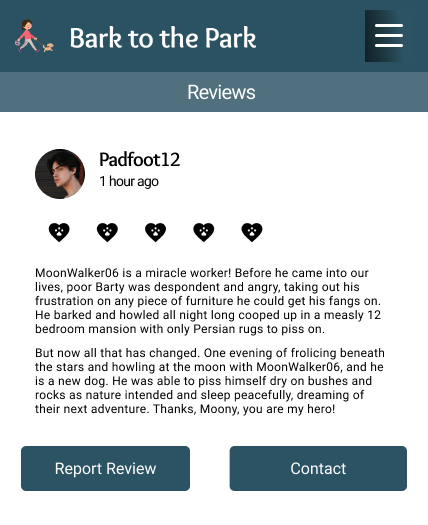
\includegraphics[height=\textheight]{Review RegularFont}\hfill}
 
``So, is it a good review?'' Lily asked, interested.

``Oh yeah, it's a good review. He's also uploaded a profile picture. Lily, you have to see this.'' He passed the phone back to her.
\vfill\hfill\pawsContinue

{\hfill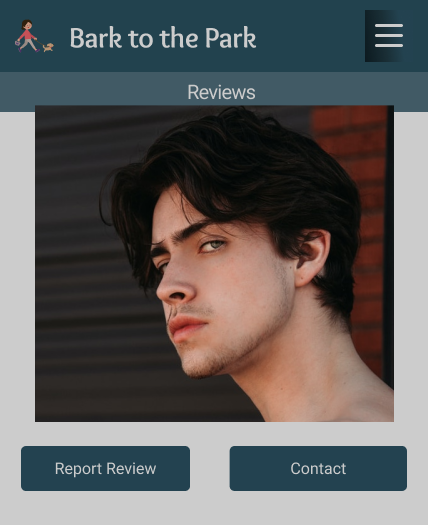
\includegraphics[height=.9\textheight]{photo overlay}\hfill}

``Oh Remus, he's gorgeous! And that review! He is definitely flirting with you.'' She was looking at the picture carefully, suddenly looking thoughtful. ``I'm pretty sure I've seen him before. Wait a minute!'' She set down the phone and started rustling around in her messenger bag, pulling out a magazine and flipping through the pages. ``Ah ha, isn't this him?''

She showed Remus a full page ad for Sleakeazy's shampoo ``for men'{}'. Featuring a very handsome man with dark hair and gray eyes. He had a towel wrapped around his waist and he was running one hand through his hair and smiling suggestively at the camera. It was definitely the same person as the profile photo uploaded by Padfoot.

``Oh wow. Do you think he just used a photo of this model to mess with me?'' Remus asked, skeptically.

``I don't know, I mean he does live in Godric's Hollow. Doesn't the owner of Sleakeazy's live there? It could really be him. And he likes you, Remus! You should go for it!'' She shoved him playfully. 

Remus just shook his head and tutted, ``No, no, he's a client, Lily. Best to keep things professional. I really should send him a message to thank him for the review though.'' He grinned, and Lily snickered as he started typing out a message.

\smsConversation{Padfoot}{
	\smsTo, {Moony}, {Wow, Padfoot, I don't know what to say. Thank you for the glowing review. I'm already getting more jobs lined up.};
	\smsFrom, {Padfoot}, {You deserve it, Moony. Barty was raving about you.};
	\smsTo, {Moony}, {Barty is actually a really well behaved dog. He's definitely been trained. You said he isn't yours?};
	\smsFrom, {Padfoot}, {No, he's my brother's. I'm not really a dog person. At least not small dogs. I prefer them big, fluffy, and with lots of drool. Honestly, I think I was just traumatized as a child by a horrible hairless chihuahua of my mother's.};
	\smsTo, {Moony}, {LOL Okay, it all makes sense now. I love all sorts of dogs, but even I find hairless chihuahuas disturbing. \emoji{grimacing-face}};
	\smsFrom, {Padfoot}, {He was a creepy little gremlin named Kreacher. He hated me, growled and snapped at me whenever I came near. I have no idea why. I'm obviously delightful! He loved my mother and my brother though, would follow them around and act all innocent for them. Little bitch.};
	\smsFrom, {Padfoot}, {I imagine Kreacher has ``crossed the rainbow bridge'' by now. Mother probably had him stuffed and mounted on the mantelpiece, knowing her. *shudders*.};
	\smsTo, {Moony}, {\emoji{face-screaming-in-fear} Thanks for the mental image to haunt my nightmares, Padfoot.};
	\smsTo, {Moony}, {Got to go, duty calls.};
	\smsFrom, {Padfoot}, {\emoji{pile-of-poo}}
}

Over the next week, messages from Padfoot were few and far between. Remus started to think maybe he had imagined the connection he felt in their easy banter of the first couple of interactions. Still, he couldn't help the queasy nervous excitement he felt when he went to Godric's Hollow each night, hoping that Mr.\ Black himself would come out to greet him with Barty. It was silly, but he found himself taking more time grooming himself, even putting on cologne, and choosing his most whimsical socks to wear. He imagined Padfoot would tease him about them if he saw them. It was a pathetic little fantasy, he realized. And every night, he felt the sting of disappointment when it was Shackelbolt who greeted him at the gate, with Barty leashed up and ready for his walk.
 
He would try to think of clever or witty things to say to start the conversation again, but usually he chickened out. One time, he even used the app's defecation tracking feature to outline a giant poop emoji over the map of the park. Padfoot had reacted to that with a string of emojis and compliments which made Remus feel ridiculously giddy for the rest of the night. He found himself re-reading the conversations during boring lectures and bus commutes.

Get a grip on yourself! Remus groaned, sinking into his desk as he tried to will himself to focus on his text book. This was ridiculous. He had a crush on a fucking male model, who lived in a mansion, and whom he had never actually met. Even if they did meet in person, there was close to zero chance that Padfoot would be interested in him. He couldn't let this distract him from his studies. He put his phone away and returned to his notes.

\dogPrintRule

\textbf{Sirius} 

Sirius knew that there was nothing wrong with same-sex attraction. He knew that it was okay to be gay. He knew, because wonderful people like Mr.\ and Mrs.\ Potter had told him so. He knew, because Dr.\ Pomfrey had told him so. He knew, because he had great friends like Marlene McKinnon and Dorcas Medowes, who were gay, and definitely were not perverts, or suppressive persons. He knew that! But something in him still struggled to believe that there wasn't something fundamentally wrong with him. You would never know that he was incapable of being in a relationship, because Sirius Black had been well trained on how to act around people. He knew how to flirt and smile and flatter. But whenever he had actual feelings for someone he was flooded with fear and shame. It was probably just his reactive mind --- NO, not reactive mind, Sirius cursed to himself. It was ``trauma''. Religious trauma. That was the term Dr.\ Pomfrey would use to describe these intrusive thoughts and emotions. And she was a real, college-educated psychiatrist. And reactive minds, and body thetans, and tone scales, and suppressive persons were all bullshit made up by a madman.

He reminded himself of all of these things over and over as he showered and scrubbed himself clean, trying to force himself out of his own head. And as he dried himself off and headed to the closet to get dressed, he picked up his phone and dialed Marlene's number.

``Marls, we're going out tonight. What's that gay bar you were telling me about?''

Marlene whooped, ``Yes, Sirius, finally! It's `The Hog's Head'.'' He made a derisive sound at the name of the bar. ``I know it sounds gross, but it's a fun place. The owner's a little weird but he's not stingy with the liquor in the mixed drinks! I'll send you the address.''

\dogPrintRule

\smsConversation{Moony}{
	\smsTo, {Padfoot}, {\emoji{grinning-squinting-face}\emoji{grinning-squinting-face}\emoji{grinning-squinting-face}\emoji{rolling-on-the-floor-laughing}\emoji{rolling-on-the-floor-laughing}\emoji{beaming-face-with-smiling-eyes}\emoji{beaming-face-with-smiling-eyes}\emoji{face-screaming-in-fear}\emoji{face-screaming-in-fear}\emoji{yawning-face}\emoji{zipper-mouth-face}\emoji{anguished-face} \emoji{face-with-monocle}\emoji{pile-of-poo}\emoji{pile-of-poo}\emoji{pile-of-poo}\emoji{winking-face-with-tongue}};
	\smsTo, {Padfoot}, {OMG MOONY YOU MAD GENIUS};	
	\smsFrom, {Moony}, {I have no idea what you are referring to, Padfoot.};
	\smsTo, {Padfoot}, {\smsPic{poopmap}{}};
	\smsFrom, {Moony}, {Oh right, yeah I meant to ask… What have you been feeding this dog??};
	\smsTo, {Padfoot}, {I told Prongs vegan pet food was a bad idea! He's clearly crying out for help.};
	\smsTo, {Padfoot}, {I'm so sorry you have had to deal with all this shit, Moony. You are an angel\emoji{baby-angel}};
	\smsFrom, {Moony}, {I am going through poop bags at an alarming rate. I assume I can just submit an expense report for reimbursement? \emoji{money-with-wings}};
	\smsTo, {Padfoot}, {\hspace*{0.2\textwidth}\includegraphics[trim={0 7cm 0 2.5cm},clip,width=0.6\textwidth]{Screenshot\_20220615-103936}};
	\smsTo, {Padfoot}, {Don't you even worry about that, I'll make sure you are fully stocked.}
}

``Hey, you! Yoohoo, Black. Did you beg us to come out tonight just so you could stare at your phone?'' Marlene gave him a small shove and leaned over the bar, waiving the bartender over to refill her drink. 

``Well, it's not like much is happening here.'' He turned on the stool and gestured to the nearly empty bar. He nodded and raised his glass to Dorcas, who had just taken an impressive shot in a game of pool she was playing with some bar regulars.

``It's still early, this place really picks up after 10. But that's not the important thing. The important thing is for you to tell me who is putting that dopey grin on your face.'' She circled a finger in front of him, her voice already a bit slurred from the alcohol.

``What are you talking about? This is just a regular grin.'' he scoffed, waving her hand away. 

``Who do you think you're talking to, Black? I've been photographing that face since we were 15. I know all of your smiles, and that one is special. So, tell me who he is so I can hire him to come and hang around the set for our next photo shoot.'' She nudged him, gesturing to the phone.

Sirius gave an exaggerated sigh, ``It's just my dog walker. If you must know, McKinnon.''

``Your dog walker?'' she whooped, and grabbed his arm, ``Oh my god, Sirius, tell me you're hitting that!'' He really didn't see what she found so amusing about it.

Sirius felt an uncomfortable heat rising from his belly, and he knew his face was flushed. He was glad for the dim lighting in the bar. ``I haven't even met him. He just sends me updates about the dog, and he's kind of funny. That's all.'' He knew he sounded defensive. He also knew Marlene wasn't buying it for one second. 

``Alright.'' She had stopped laughing, and was looking at him with concern in her eyes now. ``So why haven't you met him?''

Sirius stared at his beer for a while before answering. ``I don't know. I will. Just not yet.''

Marlene leaned over and wrapped an arm around him, laying her head on his shoulder. ``Oh, sweetie. That's okay, you'll get there. You just take your time.'' And he felt his body relax, wiping away tears that he hadn't even noticed he was holding back.

\chapter*{Chapter 6}

\textbf{Sirius} 

Sirius woke with a pounding headache and an acrid taste in his mouth. He couldn't remember if he had brushed his teeth before passing out in his bed. He could barely remember stumbling into the house after his evening at the bar. Marlene had been right about the heavy pours at the Hog's Head. She was also right about the atmosphere picking up later in the evening. The bar had become crowded and loud and Sirius had found himself dancing with attractive strangers and letting them buy him cocktails until his mind was numb and shameful thoughts were pushed aside and there was only the beat of the music and the warm bodies pressing against him and the burn of the alcohol in his throat.

He stretched, feeling his leg bump into a warm weight snuggled up against him. He stilled for a moment as the small body squirmed and settled back into sleep. Barty. Sirius smiled and carefully stepped out of the bed, trying not to disturb the dog again. Barty really had become more tolerable now that he was being taken on morning jogs with James and evening walks with Moony. He still had a lot of energy, or course. He had a bright green rope with a red grip on it that he would drag around with him, and when he wanted to play tug of war he would hold it in his mouth and jump at Sirius's feet with his little tail wagging expectantly. He usually indulged the dog by tugging on the rope, eventually pretending to let Barty win, or else taking the toy and throwing it across the room to make him fetch it. Sometimes, when he looked at Barty curled around his favorite toy on his pet bed fast asleep, he didn't even think about Regulus or feel the pit of rage and regret that the thought triggered in his stomach. Sometimes.

He took some Advil and a long shower before settling himself at the kitchen table with a large mug of coffee and a container of leftover chinese takeout. He unlocked his phone to scroll through his social media alerts while the caffeine and greasy food started to work their magic on his hangover. His phone dinged with the familiar sound indicating a text message, and his heart gave a little jolt when he saw that it was from Moony.

\smsConversation{Moony}{
\smsTo, {Moony}, {Padfoot, I'm so sorry, but I have to cancel my walk with Barty tonight. Something came up. I'm really sorry.};
\smsFrom, {Padfoot}, {You don't need to apologize. Do what you need to do. I hope it's nothing bad?}
}
It took a while for Moony to respond and Sirius quickly regretted the question. What right did he have to ask about why he had to cancel? It wasn't like they were really friends. They barely knew each other, for god's sake. It was none of his business. He was thinking about sending an apology when his phone dinged again. 

\smsConversation{Moony}{
\smsTo, {Moony}, {Well, it isn't good.};
\smsTo, {Moony}, {It's my mom. She isn't well. Hasn't been for a long time, but it's taken a turn for the worse and I just really need to be there with them.};
\smsFrom, {Padfoot}, {Of course. I'm so sorry to hear that. I know what that's like. Go and be with your parents, Moony. I wish there was something I could do to help.};
\smsTo, {Moony}, {Well, I have a 40 minute bus ride to imagine every horrible outcome. I could use a distraction… Have any funny stories?};
\smsFrom, {Padfoot}, {Yeah, okay, funny stories, I can do that! Just give me a minute.};
\smsFrom, {Padfoot}, {So, when I was a teenager, my parents sent me to a boarding school in L.A. A ``performing arts'' school. A real fancy one, where the celebrities send their kids.};
\smsFrom, {Padfoot}, {My best friend really wasn't interested in performing arts at all. I think his parents just sent him there because some of their friends told them it was a good school. But he and I were easily bored and usually looking for ways to cause trouble.};
\smsFrom, {Padfoot}, {We had this horrible class on Etiquette. Our teacher was a real piece of work. I swear she actually hated teenagers with a passion. She would dole out punishments for the slightest thing. If a girl in the class would giggle, or if a boy showed up with his shirt untucked, she would tut about how ``inappropriate'' it was and assign detention. Oh and she had this high pitched voice and spoke in a fake posh british accent, it made my skin crawl.};
\smsFrom, {Padfoot}, {She would wear these big pink bows in her hair, and I swear to god Moony, she looked like a toad. I'm not being cruel, facts are just facts.}; 
\smsFrom, {Padfoot}, {One day we were going to have a lesson on table manners, so they had set up a table like some English tea party. They had put out trays of sandwiches and tea cakes. You know the serving trays with the silver covers over them like they have at hotels.};
\smsFrom, {Padfoot}, {It had been rainy and muddy out, so my friends James and Peter and I brought a shoebox outside and started digging up worms and filling the box with them.};
\smsTo, {Moony}, {Oh I think I see where this is going \emoji{frog}\emoji{worm}};
\smsFrom, {Padfoot}, {Shh \emoji{shushing-face} patience moony, I'm telling a story here};
\smsFrom, {Padfoot}, {We snuck into the classroom early and started putting handfuls of worms under the serving lids. We must have miscalculated how much time we had, because the bell rang and people started coming into the classroom. So, we jumped into our seats and started frantically wiping our hands on the table cloth under the table. That's when I noticed the panicked look on Peter's face.};
\smsFrom, {Padfoot}, {Well, Umbridge (that's toad face) noticed his squirming too, and was joyfully assigning him detention when she opened the lid of one of the serving trays. She started shrieking, and other kids were lifting their serving lids and more girls started shrieking, and before you knew it, the classroom was filled with glorious pandemonium.};
\smsFrom, {Padfoot}, {Prongs (that's James) and I were literally rolling on the floor laughing. Especially when Pete finally stood up and we saw why he was squirming. He had sat directly on the box of worms. When he got up, his ass was covered in squished and squirmy worms and he was mortified!};
\smsFrom, {Padfoot}, {And that's how Peter got his nickname, Wormtail. He would never live that one down.};
\smsTo, {Moony}, {\emoji{face-with-tears-of-joy} Brilliant. I'm sure you all learned your lesson in detention?};
\smsFrom, {Padfoot}, {Fat chance. We did the same thing a week later, but even better, we used actual toads. Harder to procure, but worth it for the payoff.};
\smsTo, {Moony}, {\emoji{rolling-on-the-floor-laughing}\emoji{rolling-on-the-floor-laughing} That's amazing. You were naughty, weren't you? So if that's how Wormtail got his nickname, what about Prongs?};
\smsFrom, {Padfoot}, {Ah, well it's not as funny of a story, but it's from the same class. We had to learn to tell forks apart by the number of tines. That was the word we used, but James kept using the word ``prongs'', like ``Which one has only 3 prongs?'' And I would laugh at him and tell him ``They aren't ‘prongs', idiot, their ‘tines''' and he would tell me
``they are too ‘prongs''' and then he would poke me with a fork and I would shout ``stop poking me with your prongs!'' and Umbridge would give us both detention. This happened multiple times.};
\smsTo, {Moony}, {I'm at the hospital now. Thank you for the story, and the distraction, Padfoot. I mean it. It really helped. \emoji{smiling-face-with-smiling-eyes}};
\smsFrom, {Padfoot}, {Any time, Moony.}
}
\dogPrintRule

\textbf{Remus} 

Remus watched his mother, motionless except for her labored breathing with a tube down her throat. Her body was hooked up to machines and IVs, and her face was pale, almost waxy. He could hardly believe that just a few weeks ago he sat in this same chair while she teased him about being too skinny. 

She had gotten an infection. Just a minor thing, like a cold, that turned into bronchitis. Her body couldn't fight it. She had no immune system left to clear the invading bacteria. And so her fever spiked and the doctors were afraid she would not be able to recover from it. The hospital had contacted his father, Lyall, and advised that she be put into a medically induced coma to allow the heavy dose of antibiotics they were pumping into her body to do their job. There was a chance she wouldn't wake up again and they wanted to make sure he knew the risks. Everything was a risk. Every medication, every therapy, they always wanted to discuss the risks first. As if they really had a fucking choice. What was the alternative? Do nothing and let her die?

His father was here now. He was sitting in another plastic chair across from Remus, holding his wife's hand and whispering to her as though she could hear him and understand. Maybe she could, but Remus doubted it. Lyall Lupin looked as weary as Remus felt. Remus knew that his father had been spending his meager pension on cheap beer and cigarettes and ignoring the piling up of bills and phone calls from debt collectors. But when he looked at his wife, there was actually hope in his eyes. Like he really believed she would get better. That she would come back to him. He must have had to believe that, just to keep getting up in the morning.

Remus unlocked his phone to check his University email account. He had notified some professors and a study group that he would be missing classes for a couple of days. He needed to contact his advisor too, to see about making up some missed field experience hours. He ran a hand through his hair, it had gotten too long. When was the last time he had a trim? He let out a frustrated breath, feeling overwhelmed and struggling to think of what to type to his advisor, when Lyall interrupted his thoughts, speaking softly. ``Son, you look exhausted. Why don't you head back to the apartment and rest a bit. Or take care of your school business, whatever you need to do. I'll be okay here with your ma.''

Remus looked up, considering him carefully. He nodded. ``Alright, but call me if there's any change. I mean that, any change.'' And he stood and put his hand on his father's shoulder. He patted it and smiled sadly. ``Of course, son. Don't you worry. Go on, now.''

His parents' apartment was only about a mile from St.\ Mungos, so he walked there in less than 15 minutes, using his key to let himself in. It smelled of stale beer and cigarette smoke, and a little bit of moldy food. The kitchen sink was overflowing with unwashed dishes. Remus groaned, he really didn't have the energy to clean up his dad's mess right now. So instead, he grabbed a cold beer out of the refrigerator and went out on the tiny balcony patio and settled himself into a sun faded folding camp chair.

He unlocked his phone again to get back to responding to emails, when he noticed a new message from Padfoot

\smsConversation{Padfoot}{
	\smsFrom, {Padfoot}, {I decided to walk Barty myself tonight. I tried to follow your usual path from the map on the app, and he seemed okay with it but I think he was disappointed by the lack of moonwalking.};
	\smsFrom, {Padfoot}, {\smsPic{dog-gdb55341e4_640}{}};
	\smsFrom, {Padfoot}, {See? All tuckered out.};
	\smsFrom, {Padfoot}, {I hope your mom is okay. I hope you are okay.};
	\smsTo, {Moony}, {thank you, you're sweet. I'm okay, really. My dad told me to go to his apartment and get some rest. I don't feel very restful though.};
	\smsFrom, {Padfoot}, {Want to talk?};
	\smsTo, {Moony}, {Yeah, I'd like that.};
	\smsText, {}, {**Incoming call from Padfoot**} 
}
\textit{Oh god.} Remus thought, \textit{he meant ‘talk' talk, like voice talk.} Somehow, that felt so much more intimate than texting. Remus could feel his heart pounding in his chest as he swiped up, answering the call. ``Hi, Padfoot.''

``Hi, Moony. How you holding up?'' his voice came over the phone, low and filled with concern. He even sounds gorgeous. Remus thought, and he let out a long breath, sinking deeper into the chair and propping his feet up on the wall of the balcony. 

``Well, let's just say I appreciate the distraction. I'm glad you and Barty are having a chance to bond, at least.'' He tried to sound lighthearted and relaxed, taking a long swig of his beer.

``Yeah, I guess he's not so bad once you get to know him.'' He sounded like he was smiling. Remus wished he could see what Padfoot looked like when he smiled.

``How long will you have him? You said you were just looking after him for a while, right?''

``Hmm.'' Sirius thought for a moment. ``For a billion years, maybe. But let's not talk about that right now. I told you earlier about how Wormtail and Prongs got their nicknames. I thought you might want to hear about mine. Padfoot.''

\textit{A billion years? What an odd thing to say}, Remus thought. But he decided it would be best to let that one go and humor him, ``I would love to hear how you got your nickname, Padfoot.''

{\textquotedbl}It wasn't my school friends who came up with that name. It was actually James's dad, Mr.\ Potter.'' He paused, as if he needed a moment to collect his thoughts. Remus waited patiently. ``I met the Potters when I was 14, after becoming friends with James at school. I was immediately welcomed at their house. It was the kind of house where everyone felt welcome, you know? Friends were always just stopping by, helping themselves to drinks from the fridge. There were always fresh cookies, and Mrs.\ Potter would always insist that you stay for dinner. I felt more comfortable at the Potters' than I ever had in my own house. I started spending weekends and school vacations with them, as much as my parents would allow.'' 

``They sound amazing.'' Remus said, encouraging him to continue.

``They really were. At my house growing up there was kind of an old fashioned `children are to be seen and not heard' mindset. I was used to staying out of the grownups' way, or else trying very hard not to be noticed. But at the Potters', they expected kids to be noisy and rambunctious. Mr.\ Potter started calling me ``Padfoot'' because I would pad around the house in my socks, trying to be quiet. He would jump and laugh and declare that I surprised him when he turned around and found me there in the room, but I'm pretty sure it was an act. I think he was trying to encourage me to relax and feel comfortable around them.''

``Seems like it worked.'' Remus said, grinning, despite his earlier mood.

``Yeah. So much so, that when my parents disowned me at 16, I knew I would be okay, because I already had another family. I moved in with the Potters with barely any discussion about it. It was just understood, the Potters were my family, their home was my home. Still haven't left, in fact.'' He took a long shuddering breath before he continued. ``We lost both Mr.\ and Mrs.\ Potter a couple of years ago. When the pandemic started, the doctors still didn't know how to handle it, and the hospitals were overwhelmed. It got Mr.\ Potter first. Mrs.\ Potter held on a few weeks longer.'' 

Remus could hear the heartache in Sirius's voice. He felt his own throat constrict from the pain of it. ``That must have been awful, losing both of them like that. For you and James. I'm so sorry.''

``Moony, I know I'm just some guy that hired you to walk his dog, but I guess I just wanted you to know that I get what you're going through. I know how lonely it can feel. You're not alone.''

Remus was really going to cry now. ``Thank you. Really, just, thanks.'' He managed to get out.

``Are you outside? Sounds like wind or something.'' Sirius asked, abruptly changing the subject.

``Oh, sorry. Yeah, I'm on my parent's patio. It's pretty close to the freeway, I think you hear the traffic noise. I just came out here to have a beer and try to relax without being surrounded by reminders of my parents.''

``Funny, I'm doing the same thing right now on my patio. It's like we're having a beer together on the porch. Cheers, Moony.''

Remus smiled, ``Yeah, this is nice. Cheers Padfoot.'' he said, and lifted his bottle as though to clink it with Padfoot's before taking a drink. And they talked for another hour about movies they'd watched and books they'd read and about the moon rising in the sky, until Remus's phone battery was running dangerously low and they both said goodnight and went inside to sleep.

\chapter*{Chapter 7}

\textbf{Remus} 

Remus was so grateful for his friendship with Lily. As an only child, he didn't have any siblings to help bear the weight of his parents' problems. But when he called her and told her about everything he was overwhelmed with, she offered to come straight over after work and help him get things under control. He washed the dishes and took out loads of trash, while she opened mail and organized the bills in order of urgency. Then, together, they made calls and arranged payment plans, strong-armed the insurance company to review medical claims, and took care of as many past due bills as Remus could manage between his dog-walking money and his father's pension checks. 

When they were finished, Remus opened two beers and they collapsed on the couch. ``Thanks again, Lily. I couldn't have gotten through all of this without your help.'' 

``Any time, love. I know you would do the same for me.'' She gave his knee a squeeze.

He looked over and smiled fondly at her. ``You know, I really would.''

``So, on to more pleasant topics. Have you met him yet?'' she asked, kicking his foot with her own.

``Met who?'' as if he didn't know who she was talking about.

``You know, the model, Sirius Black? Mr.\ Padfoot, was it? Come on, give me the details, Remus.'' She had done what only took a small amount of internet sleuthing to find that Padfoot was Sirius Black, spokesmodel for Sleakeazy and Instagram ``influencer'', whatever that meant. Remus told her about their phone conversation from the previous evening, and she watched him intently, misty-eyed, as he spoke.

``Oh, Remus. He sounds like such a sweetheart. I love this for you!'' she winked at him, taking a sip of her beer.

Remus sighed, ``I'm trying not to read too much into it. He's fun to talk to, and that's nice enough as it is.'' he leaned back, closing his eyes. ``How are you doing? Any more calls from unknown numbers?''

``No, changing my number seems to have done the trick, at least for now. I keep thinking I see his car, but I'm probably just being paranoid. I mean, Camaros are pretty popular cars, right?''

``Not in ‘synergy' green… Do you think he's following you?'' she just shrugged, and Remus leaned forward, concerned.
``Lily, I'm worried for you. Can you have the resource officer keep an eye out for you? Walk you to your car at the very least?''

``I can get an escort to my car, but I can't ask them to do anything just because I have a feeling. I haven't actually seen Severus in months. He hasn't done anything I have evidence of aside from the text messages.'' She finished off the last of her beer and set it on the table. ``Shall we head to the hospital now? Only if you're ready.'' He nodded, setting down his own empty bottle and pushing himself off the couch with a groan.

\dogPrintRule

\textbf{Sirius} 

\smsConversation{Emmeline (Emma)}{
	\smsFrom, {Emma}, {Sirius, babe! I have exciting news!!! What are you doing this September?};
	\smsFrom, {Emma}, {I'll tell you what you are doing, you are going to New York Fashion Week!};
	\smsTo, {Sirius}, {Hey Em {\textless}3};
	\smsTo, {Sirius}, {LOL that's the dream, right.};
	\smsFrom, {Emma}, {Sirius, you're not listening babe --- You are going to come to Fashion Week! Here's the deal, I was at an event with The Weird Sisters and I ran into none other than Madam Malkin herself. We got to talking and babe, you would be the perfect model for her new men's suit line, which I told her. I showed her a few pictures and she agreed. She wants you! You need to send a portfolio ASAP, I'll email ya with the details. But babe, you are a shoe-in!};
	\smsTo, {Sirius}, {Omigod Em, that's incredible! Thank you so much!};
	\smsFrom, {Emma}, {You deserve it, babe, this is going to be huge for you! Oh but fair warning there may be one small hurdle…};
	\smsFrom, {Emma}, {One of the producers of the show is Lucius Malfoy.};
	\smsTo, {Sirius}, {Oh, fuck. Well, it was a nice dream. There's no way he'll let her hire me, I'm a dangerous suppressive. \emoji{sad-but-relieved-face}};
	\smsFrom, {Emma}, {Malkin is on your side though, she thinks the Scientologists are wackos so she's willing to fight for you. But your portfolio needs to blow the rest of the board away. And it will, you are seriously perfect for this job, hon. Screw Malfoy, you got this!!! \emoji{thumbs-up}\emoji{raising-hands}\emoji{flexed-biceps}\emoji{hugs}};
	\smsTo, {Sirius}, {Thanks for the heads up, and Em thanks for everything really. If this works out I owe you big!}
}

\smsConversation{Marlene}{
	\smsTo, {Sirius}, {Marls, what are you doing tonight?};
	\smsFrom, {Marlene}, {No plans, did you want to hit up the Hogs Head again?
	\emoji{winking-face-with-tongue}\emoji{tropical-drink}\emoji{clinking-beer-mugs}};
	\smsTo, {Sirius}, {LOL I'm still recovering from last time!};
	\smsTo, {Sirius}, {Actually, I need some help putting together a portfolio for Madame Malkin to apply for NY fashion week. Emma says she wants me, just need to impress the board enough and I'm in};
	\smsFrom, {Marlene}, {Shit, Sirius, that's huge! Of course I'll help you. Meet at the studio in an hour?};
	\smsTo, {Sirius}, {Hell yeah, on my way!}
}

\dogPrintRule

\textbf{Remus}

Lily gave Remus a ride back to his University housing. His mother was in ``stable'' condition, and there wasn't any more he could do there. But it still wasn't going to be easy to try to go about his daily life, just waiting for another phone call if and when her condition changed. It was like a constant weight on his chest, an anxiety that gnawed at him making him simultaneously exhausted and jittery. Or maybe that was all the coffee. Anyway, he had plenty to keep him busy if he could just keep going through the motions. Just keep moving. It helped time pass.

He had a new client, an elderly woman named Hepzebah Smith, who's home was conveniently located next door to the Potters' mansion. He had a feeling it wasn't a coincidence. He learned later that he was right. It had been James Potter who, upon helping his elderly neighbor with her groceries, discovered that she was in need of a dog walker for her two miniature poodles. He told her about the app that his friend had used and helped her set it up on her phone and send a request to Moonwalker06. It was perfect, because she was okay with him walking her dogs together with Barty at their usual 8:00 time slot. 

The poodles, named Hokey and Pokey, were well groomed and had the typical poodle cut, with their faces and the base of their tail trimmed short, with the rest of them covered in poofy, curly hair. They were not as well trained for walking as Barty had been though, and often yanked the leash excitedly when there was some scent that caught their attention. Or another dog. Or a car. Or a bird. Almost anything, really. Still, he was managing all three dogs quite well. It was on the third night walking with Hokey, Pokey, and Barty when he saw Alecto and Amycus on the other side of the park. 

He had met the pair on previous walks with Barty. Alecto, Allie for short, was a tall sturdy woman, who had seemed stern and standoffish at first when her boxer, Amycus, had lunged toward Barty and she yanked him back and yelled at Remus to control his dog. Barty, meanwhile, had been perfectly under control. But Remus picked him up and apologized politely, introducing himself and allowing Amycus to sniff his legs and he calmed down, even allowing Remus to pat him on the head.

So Remus should have been expecting what happened when Amycus encountered Hokey and Pokey. He should have known that the boxer would lunge at the poodles. He should have known that they would tug suddenly toward the larger dog. But he wasn't prepared, and he stumbled, tripping over some path edging stones and putting out his arm to catch himself as he fell. It was like the world went into slow motion as he went down, the leashes escaping his grasp. Pain shot up his legs on impact as his knees hit the ground, tearing his jeans as well as the skin underneath. Amycus had also escaped Allie's grasp and Remus could hear her shouting as all four dogs collided in the center of the park. Barty had already become protective of the poodles and jumped in front of them, teeth bared, but it was Amycus's teeth that caused the damage. By the time Remus had picked himself up and run to the dogs, Barty was bleeding and whimpering. Allie was still yelling profanities at Remus and the dogs, but he paid her no attention as he quickly pulled out his phone, shaking from adrenaline and pain. His wrist and forearm were scraped and bloody, but it had protected his face from injury. The poodles were still tugging as Amycus walked away and Remus held Barty to his chest as he dialed Padfoot.

\textbf{***calling Padfoot***} 

``Moony! What's up?'' Sirius sounded so happy when he answered, Remus's heart skipped and he almost forgot why he called. Then Barty whined and he remembered the urgency of the situation.

``Padfoot, I'm sorry to bother you… We had an incident with another dog at the park. Barty's bleeding. I think I need to get him to the pet hospital.'' It all came out in a rush, and Sirius picked up on the panic in his voice.

``Okay, don't worry. There's a pet hospital just a couple of miles from there. I'm in the city right now, but James is home. I'll have him come and get you and I'll meet you at the vet. Sound good? Moony, are you okay?''

Remus took a deep breath, Sirius's calm helping him relax. ``Yeah, I'm a little scraped up, but I'm okay. I'm just worried about Barty. I have Hokey and Pokey with me, too.''

``That's okay, no problem. Where should he pick you up?''

``Corner of Hogsmeade and Central.''

``Okay got it. I'll see you soon.''

James Potter arrived five minutes later. He drove a maroon colored SUV that looked almost black under the yellow light of the street lamps. He stepped out of the car to quickly help Remus and the dogs pile in. He was a few inches shorter than Remus, and with a broad build and brown skin. He wore glasses with thick black frames, and his black hair stuck out in every direction. Remus laughed inwardly at this, remembering that he was the owner of a company that began with a taming hair gel. He had a friendly and calming demeanor which instantly put Remus at ease. By the time they got to the pet hospital, only a 5 minute drive away, James already felt like a trusted friend. He offered to take Hokey and Pokey home to Mrs.\ Smith, and gave Remus his number, just in case he needed anything.

It was nearly nine o'clock when Remus walked into the 24 hour animal hospital. The reception area was empty of people, but he could hear a bird chirping and a dog yipping somewhere behind the doors of the reception room. Remus tapped the bell on the counter to signal that there was a patient awaiting help. A minute or so later a man with a shaggy beard that was barely contained in a beard net and long curly hair tied back in a ponytail, and wearing brightly colored surgical scrubs, opened the door and looked around, his eyes falling quickly on the whimpering, bleeding dog in Remus's arms. He was a large man, at least 6'10'' by Remus's estimation. Remus himself was 6'5'', usually the tallest man in the room, but this man towered over him. He was not scrawny like Remus, either. He was quite wide as well, and had such large hands that he could hold Barty in one of them with room to spare. He didn't though, he took him carefully with two hands and held him with such care and tenderness that Remus felt the knot in his stomach start to release instantly, knowing that the dog would be well cared for. He introduced himself as Dr.\ Rubeus Hagrid, handed Remus a clipboard with paperwork but invited him back to the exam room and began tending the wound without waiting for the paperwork to be completed.

Remus explained the incident that had caused the injury and told Dr.\ Hagrid that the dog's owner was on his way. The doctor didn't seem too concerned about the paperwork, focused entirely on Barty. He gave him a sedative and cleaned the wound, explaining that he would need to stitch it up, and keep Barty overnight, but he would be just fine. Remus started to feel light headed from the strange smells of the animal hospital and from watching as Dr.\ Hagrid tended the wound. He thanked the doctor, and asked if it was alright if he went outside for some fresh air for a bit to clear his head. And that's where he was when he heard the rumble of a motorcycle pulling into the parking lot. And when he looked up, there was Sirius Black, running his fingers through his thick dark hair and grinning at him. 

\chapter*{Chapter 8}

\textbf{Sirius} 

Sirius had already put together some of his recent videos and photos from social media, and Marlene had many more studio photos to give them options for putting together the perfect portfolio to send to Madame Malkin's team. They had spent a couple of hours pouring over the photos and were pretty satisfied with what they had accomplished by the time Sirius got the phone call from Moony. Marlene assured him that she could finish this up and send it off for him and he should go to take care of his dog.

When he pulled up to the animal hospital on his motorcycle, he saw Remus leaning on the wall to the right of the entrance, hands in his pockets looking down at his feet. He was tall and skinny, wearing the same knit beanie he had on in his profile picture, but his hair was longer and he could see light brown locks softly curling under his ears and along his neck. He was wearing a dark gray t-shirt which was stained darker in the chest with what Sirius realized with a jolt must have been blood. His faded jeans were torn at the knees. He looked up and met Sirius's eyes as he removed his helmet, quickly ran a hand through his hair and grinned nervously. Remus was watching him, his expression unreadable. It made Sirius's stomach flutter and he was suddenly very self-conscious. He parked his bike, stowing his helmet, and hoped he didn't look nervous as he strolled over to meet Remus.

``Moony?'' he said tentatively, looking up through his long lashes at the taller man.

Remus breathed out a small laugh and smiled shyly, ``Yeah. Um, hi.''

``Hi.'' Sirius replied, taking in the man in front of him. He had light brown eyes and tan skin, with the hint of a shiny scar near his left eye. He appeared to have left his beard unshaven for at least a couple of days, the stubble the same light brown as the soft curls on his neck. Now that he was up close, Sirius noticed his arm was scraped up and covered in blood and dirt. ``Shit, Moony, are you bleeding?''

Remus seemed to take a second to register what he had said, finally looking away from Sirius's face to his own arm. ``Oh. Um, maybe a little. Most of the blood is Barty's though. He's okay, the doctor is patching him up now. He wants him to stay overnight for observation, but he's going to be okay. Just need you to fill out some paperwork. I'm so sorry, I'll pay the vet bill, obviously.'' Sirius put his hand on his shoulder, shushing him and shaking his head.

``Remus, no, it was an accident. Look, I'll go in and take care of the paperwork and talk to the doctor. Then would you like to come back to the house with me? We can clean up those cuts. And you look like you could use a drink.'' He smiled reassuringly and gave his shoulder a squeeze, removing his hand only once he saw Remus had visibly relaxed, letting out a long breath, and smiling back for the first time.

``Yeah, that sounds good. Thanks.'' he nodded, pulled open the door and waited for Sirius to enter, following him into the reception area.

Sirius started filling out the forms, glancing up at Remus every once in a while, very aware of his presence. He sat in one of the chairs next to the window, leaning to look out with his hand up to his face, absentmindedly chewing on his thumbnail, and his leg was bouncing with nervous energy. Sirius thought he looked so young and vulnerable and his heart ached with a desire to protect and comfort him.

Only ten minutes later, Sirius was handing Remus his spare helmet. ``Have you ever ridden a motorcycle before?'' he asked, watching as the other boy shoved his beanie in his pocket and put the helmet on his head, fumbling with the straps.

``You probably won't be surprised to hear that I have not.'' Remus looked a little apologetic as Sirius laughed and helped him adjust the helmet and held his arm as he climbed onto the seat, showing him where to prop his feet.

Sirius pulled on his own helmet and positioned himself on the bike, calling behind him, ``You're gonna want to hold on to me. Don't worry, I don't bite!'' he teased as Remus reluctantly wrapped his arms around his torso.

``Oh god, this was a terrible idea. How did you talk me into this?'' Remus moaned.

``People say I'm very persuasive.'' Sirius laughed and called back ``Okay, Moony, hold on tight.'' before starting up the engine. He could feel Remus's heart pounding, and the warmth of his chest pressed up to his back as they pulled away from the pet hospital and onto the road back toward Godric's Hollow.
\smsConversation{Prongs}{	
	\smsFrom, {Prongs}, {I dropped Remus off at the pet hospital.};
	\smsFrom, {Prongs}, {Sirius, he's so sweet. You need to make him our friend.};
	\smsTo, {Sirius}, {I'm way ahead of you, already invited him over. I just need to fill out a couple of forms then I'm bringing him to the house to clean up his cuts and have a beer.};
	\smsFrom, {Prongs}, {Oh good, I'll find a clean t-shirt and some gym shorts for him so he can get out of those bloody clothes.};
	\smsFrom, {Prongs}, {Think Remus likes IPA? NVM I'll just bring up a variety from the basement fridge. See ya soon!!\emoji{clinking-beer-mugs}};
	\smsTo, {Sirius}, {Anything is fine, thanks Prongs!}
}
\dogPrintRule

\textbf{Remus} 

Remus held on for dear life, less conscious of the fact that he currently had his arms wrapped around the waist of Sirius Black than he was of the huge rumbling machine that seemed to lean dangerously when they turned the corner. Sirius must have had a remote control that he didn't see, because the gate opened up for him when they got to Godric's Hollow, and he drove up around the side of the mansion and pulled into a huge garage, which also seemed to sense his approach, opening up with perfect timing. Once they were safely parked, Sirius took Remus's arm and helped him dismount, asking if he was okay, and not letting go until he was sure Remus was steady on his feet.

They walked into a wide hallway that opened up to a bright living room. It was decorated sparsely, very clean and modern. Remus found it hard to believe it was home to two young bachelors, but he supposed it was the elder Potters who had furnished and decorated the house. James appeared from another hallway, grinning widely. ``Remus!'' He called out, heading over to them. ``Good to see you again! You want the grand tour?''

``Prongs, let the man get cleaned up first, Jesus.'' Sirius shook his head but was smiling fondly at his old friend, who was practically bouncing like an excited child. Sirius inclined his head toward a hallway to the right. ``C'mon, Moony, the first aid kit is in this bathroom over here.''

``I left a change of clothes in there for you. Get comfortable. Do you like IPAs, Remus?'' James was calling after them as they headed to the hallway.

``Yeah, sure, thanks James!'' Remus called back, following Sirius. The bathroom was so big that it had room for a chair and a small couch with a little table and a potted plant across from a long counter with two sinks. There was a jacuzzi tub and a glass shower stall in the room, and the actual toilet was behind another door. Sirius handed Remus the t-shirt and shorts James had left on the counter for him, indicating he should get changed in the toilet room.

When he came back out, his torn and dirty clothes wadded up under his arm, Sirius had pulled up the chair next to the table, the first aid kit open in front of him. He patted the seat of the little couch, and Remus sat, obediently.
``James seems like a really great guy.'' He said, trying to make conversation.

``Yeah'' Sirius said as he took Remus's arm and started cleaning it with a cotton ball with some solution on it. It didn't sting at all, it actually felt very soothing. ``He sent me a text about how sweet you are and that we need to make you our friend. So, it seems you made an impression, too.'' He smiled, not looking up from his work, his thin white fingers tenderly cleaning and bandaging the cuts and scrapes. Remus was sure Sirius could feel his quickening pulse through his warm skin, where the cool fingers gripped his thin wrist while he worked, quiet and focused. He really was as beautiful in real life as he was in magazines. Remus always assumed there was a lot of photo editing that made models look like that. But Sirius Black was the real thing. In fact, now that he had seen his genuine smile in person, he couldn't imagine why they didn't put that smile on every ad they ever printed. He could look at it all day and never tire of it. He knew that as long as Sirius would want to spend time with him, then he would do everything he could think of to bring out that smile.

``You're really good at this.'' Remus spoke softly as Sirius moved on to cleaning the cuts on his knees.

Sirius chuckled quietly, ``Well, it's real complicated stuff, Moony. Don't try this at home.'' he teased. ``Seriously though, I don't mind. I like taking care of people. I actually thought about going to nursing school. I still might, as a backup plan. I can't ride on my good looks forever.'' He glanced up and winked, making Remus's heart skip a beat. ``I learned everything I know from the best nurse in the world. Euphemia Potter, herself.'' he straightened up, closing the first aid kit. ``There you go, good as new. Shall we have that beer now?''

``Absolutely. And I was also promised a tour. I've never been in a house the size of an entire apartment building before.'' He stood and stretched, impressed at how much better he felt, no longer feeling the stinging pain in his knees and forearm.

``Well then, I shall call Mr.\ Prongs to guide you through a tour of our fine estate.'' He put on a posh accent and clapped his hands twice ``Oh Prongsy!'' he called, just as James met them coming into the living room with three bottles of beer in his hand. ``Here he is now! Mr.\ Prongs, can you please give Mr.\ Moony here the grand tour.''

``I shall, good sir.'' James bowed to them as they took their beers, and then waved them forward. ``You'll see here on the right hand side, the grand entrance hall…'' and the tour continued for four floors, at least 8 bathrooms, twelve bedrooms, two kitchens, a basement with a private gym and a rec room. There was even a private ``theater'' room in one of the upper floors. They settled on a large balcony on the third floor, overlooking the garden. There was a matching set of patio furniture, with a fire pit table in the center and a mini-fridge, fully stocked with a variety of beers and hard seltzers.

``This is the patio where I had my first beer with you, Moony.'' Sirius said as they got comfortable on a wicker couch with big blue cushions. ``Cheers!''

``Cheers!'' they clinked their bottles. ``I was on a much smaller porch. I like this one much better.'' Remus said, leaning back and propping his feet on an ottoman while taking the last swig of his beer.

``So, what do you study at UC Hogsmeade, Remus?'' James asked as he placed a few fresh beers on the patio table between them, settling himself in a wicker swivel chair.

``School counseling. I'm getting certified to be a school psychologist actually. I'm due to graduate in May, so the next couple of months will be brutal.'' He noticed an odd look pass between James and Sirius. ``Well, what do you know, a psychologist! Isn't that interesting, Sirius?'' James said, his eyes not leaving Sirius's face.

Sirius was shaking his head, still glaring at James, making Remus feel oddly uncomfortable. ``Um, did I miss something?
What is it?''

``Oh, it's nothing. I think it's great that you're going to be a psychologist.'' Sirius finally looked away from James, focusing back on Remus. ``So, what got you interested in school counseling?{\textquotedbl} He asked, a hint of apprehensiveness in his voice.

{\textquotedbl}Well, I know it's pretty much the least lucrative job possible for a psychologist, but I guess like anyone who goes into public education, I was inspired by someone who had a big impact on me when I was growing up.{\textquotedbl} He leaned forward and picked up his second bottle of beer, nodding thanks to James. When he leaned back on the couch he saw Sirius was turned to face him, one arm propped up on the back of the couch, watching Remus expectantly, waiting for him to continue.

``Her name was Ms.\ McGonagall. To be honest, I was a bit of a juvenile delinquent in my early teens. My teachers had all but given up on me. But McGonagall didn't. She helped me figure out how to deal with the trauma from something that happened to me when I was just a little kid. I had never properly processed it all. She even helped me come to terms with my sexuality, to accept that there wasn't anything wrong with me. That what I was feeling was perfectly normal. If I can be that person for just one troubled kid, like she was for me, then it will all be worth it.''

Everyone was quiet for a moment. Remus glanced over at Sirius, who was watching him, fascinated. It made him feel a bit self-conscious, and he looked back at his hands, where he was mindlessly picking the label off his beer bottle. James was the first to break the silence. ``Wow, that's beautiful, Remus. I'm sure you'll help a lot of kids, like really make a difference in their lives. Man, and I'm wasting my life working in corporate law. You, sir, are an inspiration!'' And he clinked Remus's bottle. He clearly wanted to move on to lighter topics, but Sirius had had other ideas.

``What happened to you? When you were a little kid?'' he asked, still watching Remus intently.

``Oh. Um. We were attacked. Well, my dad was the target, I was just in the wrong place at the wrong time.'' He paused, taking a deep breath and another long pull from his beer bottle. Halfway through his second beer he was starting to feel the effects. He knew it was probably prejudice, but he had always assumed that rich people were all entitled assholes. He was surprised how comfortable he felt with these two strangers, who despite growing up in the same city he did, might as well have been from a different universe. It seemed that they found him just as fascinating as he found them. They were both paying rapt attention as his life story poured out of him.

``My dad was a cop. He was good at his job. He loved it, but it was stressful. It was hard on him, on my mother, on all of us, really. By the time I was 5 years old, she had finally convinced him to take the desk job they were offering him. It was an opportunity to get him off the streets, working a respectable nine to five shift, so we could have a nice quiet family life, ya know? He would be home for dinner every night and my mother wouldn't be worrying all night that he might not make it home at all. So he did, he took that job, but he had an ongoing case for an arrest he had made. His name was Fenrir Greyback, and he was a real nasty piece of work. He ran a drug ring, and probably all sorts of other illegal shit, I don't really know the details. But I do know that he had a loyal following of gang bangers who were not happy about my dad testifying in court against Grayback. One day, we were just coming home from picking up groceries and they drove by guns blazing. Got my dad in the shoulder. But got me here -'' he pointed to the scar on the side of his face, ``and here.'' he pointed to his lower torso. ``I almost died. Spent a few months in the hospital, and had to go back twice over the next year for surgeries to fix the mess the bullet made of my lower intestines.''

``Holy shit.'' James breathed. ``Yeah.'' Remus replied. Sirius was quiet, but he had leaned forward, looking like he wanted to reach out and touch Remus's arm, but thought better of it, reaching for his beer instead.

``My dad blamed himself, of course. It was really hard on my parents. I was so young, I don't really remember the pain of being shot, but I remember the pain it caused my parents.'' He finished up his second beer and James offered him another. ``The good news is, Grayback is rotting in prison as we speak.''

``Fuck, yeah, let's drink to that!'' James cheered, and that seemed to break the dark mood. ``Man, Remus, well I'm sorry Barty got hurt tonight, but I'm glad you came to hang out with us.''

``Yeah, I'm glad, too. You guys are alright.'' Remus laughed, relaxing back into the cushion.

``You know, Moony, Sirius only hired you because he thought you were cute.'' James said, clearly feeling the effects of his third beer by this point.

``Prongs!'' Sirius flicked a beer cap at James, his face going red.

``What? It's true! You were like \textit{`Oh, he's cute, I want this one!'}'' James was really laughing now, and retaliating by flicking more bottle caps back at Sirius. Remus covered his head with his arms, hiding his own reddening face while trying to stay out of the line of fire as the battle continued.

\chapter*{Chapter 9}

\textbf{Sirius} 

\smsConversation{Moony}{
	\smsTo, {Padfoot}, {Good Morning, Moony!};
	\smsFrom, {Moony}, {Padfoot, it's 12:30. It's literally the afternoon now.};
	\smsTo, {Padfoot}, {Good Afternoon, Moony! How was your morning, then?};
	\smsFrom, {Moony}, {Good Afternoon, Padfoot. My morning was rough. It took a lot of espresso to get me through my early class. Feel pretty good now, though. Any news about Barty?};
	\smsTo, {Padfoot}, {I'm about to go pick him up. They said he is in good shape, but no moonwalking for a couple of days.
	\emoji{crying-face}};
	\smsTo, {Padfoot}, {Are you walking Hokey and Pokey tonight?};
	\smsFrom, {Moony}, {If she hasn't fired me, then yes, that's the plan};
	\smsTo, {Padfoot}, {James wants me to ask you to come over after you drop off the poodles because he already misses you, the soppy idiot.};
	\smsFrom, {Moony}, {Awww, tell James I miss him too. \emoji{smiling-face-with-heart-eyes} I'd love to come and visit him.};
	\smsTo, {Padfoot}, {I hate you both.};
	\smsFrom, {Moony}, {It's a good thing I'm so cute then \emoji{winking-face}};
	\smsTo, {Padfoot}, {Oh my god.};
	\smsFrom, {Moony}, {See you tonight, Padfoot.};
	\smsTo, {Padfoot}, {Yeah, see you then Moony.}
}

When the doorbell rang (still the damn Jingle Bells chorus), James and Sirius were in the middle of an intense game of air hockey in the rec room. James had just pulled ahead and only needed one more goal to win, so he protested loudly when Sirius abandoned the game. ``Oh, that'll be Moony, gotta go.'' he said as he tossed his paddle on the table running toward the stairs.

``Aw, come on! Well, bring him down here, I'll kick both of your asses!'' James called after him.

Sirius was out of breath when he got up the stairs, so he took a moment to try to calm himself before pulling the door open. ``Hey Moony, sorry we were down in the rec room. Come in.''

``No worries, I wasn't waiting long.'' Remus said as he stepped in. Sirius thought Remus looked amused by his obvious nervousness. Remus, on the other hand, appeared to be completely relaxed and comfortable, looking around curiously before addressing Sirius. ``Where's Barty? I'd like to see how he's doing.''

``Oh, he's in my bedroom. He's been a little lethargic. I think he's mostly annoyed about having to wear the cone. It makes him walk funny.'' Sirius laughed remembering Barty's clumsy attempts at climbing the stairs, eating at his food bowl, carrying around his rope. Really, all of his normal activities were hindered, so he seemed to think it was best to just lay on his cushion and nap most of the time. He had only needed a couple of stitches, which the vet said would come out on their own when the wound healed. Barty was supposed to wear the cone for a couple of days to prevent him from licking it and reopening the wound. Sirius was told to just check for redness or swelling twice a day, otherwise he should be back to business as usual by the end of the week.

Sirius led Remus to his room. Hearing the voice of his walking partner clearly gave the little dog the motivation to get up, and he wobbled excitedly over to Remus, jumping and twirling and yipping, demanding attention. Remus laughed and picked him up, holding him like a baby on his back and rubbing his stomach, careful to avoid the stitches. ``Who's a good dog? You are!'' he cooed.

``Wow, he really likes you!'' Sirius commented, smiling at the sweet display in front of him.

``He likes you, too.'' Remus said, sparing Sirius a quick glance, while he set Barty down and picked up his toy to play with him. Laughing at poor Barty's difficulty keeping his balance.

``I don't know, I think he can tell I'm an asshole. Dogs are good judges of character.''

Remus gave him a disapproving look. ``You are not an asshole.'' Sirius just scoffed. Remus tossed the toy to send Barty on a mission to fetch it, and turned to focus on Sirius. ``Honestly, Padfoot, you are genuinely one of the nicest people I've ever met.'' He had been standing next to the bed, and now he sat on the edge of it. ``Is this a California King?'' he asked, casually.

``Yeah, why?''

``As a tall person, I've always wanted one of these. Can I?'' He grinned, and Sirius nodded. Remus excitedly kicked off his canvas sneakers and spread himself out on the bed, arms folded behind his head. ``Yeah, this is nice, I'm not even hanging off the edge!''

Sirius climbed over him, laying on his side to face Remus, propped up on his elbow. ``How do you know you're not just a special case?''

``Hmm?''

``What makes you think I'm not just nice to you. Because I like you.''

Remus laughed, ``Well, I know I'm not the only person you're nice to. The Potters clearly loved you. I bet they thought you were nice, too.''

Sirius brushed this suggestion off, shaking his head. ``The Potters love everyone. They don't count.''

``What about your brother? He trusted you enough to take care of his dog, that's not something a pet owner does lightly, you know.''

Sirius snorted, ``Not for a Scientologist.''

Remus turned to face him, ``Your brother is a Scientologist?''

``Yeah.'' Sirius waited for a reaction to that, but Remus was just looking at him thoughtfully, maybe a little curious. They were very close to each other now, and he noticed that Remus's light brown eyes were flecked with gold. He was so lovely, it took Sirius's breath away.

``Huh.'' Remus said, ``And you're saying Scientologists don't love their pets?''

``Well, they're not supposed to, really.'' Sirius sighed, ``But you're probably right, Moony. I think Regulus does love Barty. And \textit{okay}, maybe he sort of cares about me, too.''

Remus put a hand on Sirius's arm, squeezing it ever so gently. ``Of course he does.\ \textit{I} care about you, and I've only just met you.'' And Sirius really, really wanted to kiss him. And just when he thought he might have the courage to do it, and started leaning forward ---

``Pads? Moony? Where'd you- Oh. I'm not interrupting anything, am I?'' James stood in the doorway, a stupid grin on his stupid face.

``Yes, go away, Prongs.'' Sirius snapped.

``Alright, alright. Well, when you're ready you need to come down to the rec room. I'm waiting to beat you both at air hockey, and I've got booze!''

``Hi James, that sounds great. We'll be right down.'' Remus had turned to look toward the door and wave at James.

``Traitor.'' Sirius said quietly as James was retreating back down the hall.

``You know, I really should go and hang out with James. After all, he's the one who invited me. I'm being terribly rude.''
He looked at Sirius apologetically. Sirius pouted, and Remus leaned over and kissed him. Just the slightest, sweetest touch of their lips, and then he pulled himself away, standing up from the bed and reaching for Sirius's hand, laughing
``Come on, you big baby. I'm going to destroy your roommate at air hockey.''

\dogPrintRule

\textbf{Remus} 

An hour later, and true to his word, Remus was the reigning champion of air hockey. Having easily beaten both James and Sirius twice, he decided to take a time out and plopped into a nearby bean bag chair to enjoy a cold beer and watch James and Sirius play against each other. They were much more evenly matched, but whenever Sirius glanced over at him, Remus would make a kissy face or wink suggestively, making Sirius all flustered and causing him to miss the puck resulting in a decent advantage for James. Sirius cursed and blushed furiously while James hooted and cheered.

Remus was having the time of his life. Now that he knew for sure that Sirius was interested in him, and adorably shy about it, he found it nearly impossible not to abuse his newfound power. As much as he loved making Sirius smile, making him blush was a million times better.

Once James got his seventh goal, Remus stood and congratulated him, patting him on the back. James, feeling emboldened by his win against Sirius, asked Remus for a rematch.

``I'd love to, but I really should get going. Tomorrow's a field experience day, so I need to actually have my wits about me. No skating by on caffeine like this morning.''

``Want me to give you a ride home?'' Sirius offered, eagerly.

Thinking of the motorcycle ride from the previous night, Remus quickly declined. ``No, no, thank you. I can walk.''

``Can I walk with you, then?'' Sirius asked, hopefully. His face was still flushed from the exertion of the game, and maybe a little bit from the way that Remus was looking at him. He was sweating slightly and breathing quickly, eyes dilated from the dim light in the room. Remus had to resist the urge to grab him and kiss him passionately right that very moment. Instead he said ``If you want to, maybe halfway, like to the park? Otherwise then I'd have to walk you home and we'll never get anywhere.''

Sirius smiled. ``Oh, ha ha. I'll walk with you to the park then.'' turning to James he said, ``See ya Prongs, I'll get you back in a rematch later.'' and they bumped fists.

``Alright, you two be good now. Have a good night, Moony, we'll have to hang out again soon!'' James called as Sirius led Remus out through the garage.

``Bye James, it was fun. We definitely will!'' Remus responded. And as they walked down the driveway to the gate, his boldness took over again and he slid his hand into Sirius's, interlocking their fingers. ``This okay?'' he asked quietly.

Sirius squeezed his hand a little and brushed his wrist with his thumb. ``Yeah, this is okay.'' he said breathlessly. 

``Sirius?'' Remus asked after they had been walking quietly for a moment.

``Hmm?''

``You don't have to tell me of course… but I'm curious. What happened with your parents? You said they disowned you?''

``Ah'' was all he said, and then he was quiet for a moment, so Remus kept talking ``I'm sorry if that's too personal, we don't have to talk about that.''

``No, no, Moony, it's okay. I'll tell you about it.'' He seemed to need a moment to collect his thoughts, so Remus waited for him to continue. ``How much do you know about Scientology?'' he asked.

``Not much really. I saw a documentary a few years ago. And my friend Frank once took a `free personality test' on Hollywood Blvd and complained that he kept getting mail and calls from The Church of Scientology afterward trying to sell him some expensive course about communication methods or something.''

``Ha, yeah that sounds about right. Well, you know how I told you my brother is a Scientologist? So was I. I mean we were raised in it. Third generation Scientologists. My parents were raised in it too. My grandparents on both sides joined back in the 60s. I grew up in the church, but I never felt like I fit in. It was a terrible way to grow up. They don't let you be a kid in Scientology. They say kids are just adults whose bodies haven't finished growing yet. We spent hours in courses and auditing and we never got to watch cartoons or just play with other kids. I was lucky though, I was good at talking to adults and I could charm them, and they thought I had potential to have a career in acting and modeling. If I could become a celebrity, then I would be able to spread the message for the church, help `clear the planet'.''

``And so they enrolled me in Durmstrang Performing Arts High School, and I met James, Mary, Marlene, the Prewett twins. I already knew Peter, his parents were scientologists too, so we had grown up together. He started hanging out with me and James, but he saw that I was getting off-course and saying things that were suppressive. He wrote up a knowledge report on me. My parents wanted to send me through the Rundown, it's like an intense auditing and hard labor program, but I refused. I was still a minor, so they could have made me go. But I had friends who were too high-profile by then. I already had a modeling contract with Sleakeazy. If they made me disappear, people would have noticed. So I was protected. They just disconnected with me and I was able to escape to The Potters.'' he was quiet for a moment now, taking a deep breath before he continued. ``My brother wasn't so lucky though. They were afraid I'd had too much influence on him, and they sent him off to The Ranch. It's a special school for `down-stat' kids, or problem kids in Scientology. I know it was awful for him, but I couldn't save him.''

Sirius was getting choked up now and he was pressing on his eyes trying to stop the tears from forming. Remus stopped walking and pulled him into his chest, rubbing his back. ``Hey, it's okay, it wasn't your job to save him. It's not your fault.''

Sirius took a shuddering breath and tried to calm himself, his face still pressed against Remus's shoulder. ``I was raised to believe that everything's my fault. Everything bad that happens to me, or to people I love, it's my fault. I know it's not true, but I still feel like I abandoned him. If I hadn't left, maybe I could have protected him.''

Remus touched his face aiming it up to look him in the eyes. ``No, Padfoot, you were just a kid yourself and someone offered you help and you took it. You did the right thing. You did what you needed to do to protect yourself.''

``Yeah, I suppose so.'' He wiped his eyes again. ``Sorry for getting all emotional.''

``It's fine, really.'' They started walking again. ``So, um, where is your brother now?''

``I wish I knew. He joined the Sea Org. I have no way to find him and nobody at the church will talk to me because I'm labeled a Suppressive Person. I wish I could speak to him again, but it just feels so hopeless.''

``I'm so sorry.'' Remus gave his hand a squeeze. ``Well, we're at the park now. I guess this is where we say goodnight?'' he asked tentatively, not yet letting go of Sirius's hand.

``You can't go yet, you need to show me your moonwalk!''

Remus laughed, ``Wait, are you serious?''

``I'm always Sirius,'' Sirius winked at him, and Remus laughed again.

``Okay, okay. Cool, but not right here. For you, it needs to be special.'' He looked around thoughtfully. ``Ooh, I know! C'mere.'' He tugged Sirius toward the big fountain in the center of the park.

The fountain was a garish monstrosity donated by Godric Gryffindor at the park's founding 150 years earlier. It consisted of four Centaurs aiming arrows into the center of the fountain where a tall man in a fantasy style wizard's robe and a pointy hat was pointing a wand toward the sky. Water shot out of all of the arrows and the wand, as well as various spouts of water encircling the wizard. The fountain was contained by a four foot tall concrete bowl with a narrow curved ledge. Remus finally released Sirius's hand and jogged over to the fountain, pulling himself up onto the ledge.

``Moony! What the hell?'' Sirius called to him.

Remus pointed at him, and doing his best Michael Jackson impression, he spun on the spot and smoothly moonwalked along the ledge of the fountain, finishing with another spin and the signature crotch grab with one hand on his bowed head. Sirius was doubled over laughing and applauding at the base of the fountain. Remus jumped down and headed straight for a cement picnic table, hopping up on the bench in one leap and repeating his moonwalk performance down the bench. Then he sat on the table, his legs dangling off the end and leaned back on his hands waiting for Sirius to come to him, still catching his breath from laughter.

Sirius came up close, so that his hips were between Remus's knees, and he put his arms around his shoulders. ``That was amazing, Moony. How is it that you are so good at everything?'' he said, his eyes filled with admiration.

Remus scoffed, ``I'm not good at everything. But okay, air hockey and moonwalking are my top skills.'' He leaned forward and started leaving small kisses along Sirius's jaw, moving toward his neck. ``They're right at the top of my resume. Going to make me rich someday.'' Sirius moaned quietly, tilting his head to expose more of his perfect neck to Remus's lips. ``Hmm, would I get you in trouble with your boss if I left a mark here?'' Remus asked as he lightly nipped at the delicate skin.

``Nah, but my makeup artist and photographer would never let me hear the end of it.''

Remus pulled back a little so he could look at Sirius's face. ``Really?''

``Yeah, don't worry, they're my best friends. I actually can't wait for you to meet them. They're going to love you.''

``I'd love to meet them. I know my friend Lily is going to be asking about you when I see her tomorrow.''

``Oh? And what will you tell her?''

``The truth, that you're way out of my league and I don't stand a chance.'' Remus said as he went back to work at Sirius's neck.

``So a lie, then?'' Sirius turned to meet Remus's lips, kissing him deeply, one hand tangling in his curls, the other hand pressing into his back as if he could bring their bodies any closer together.

``It's late, I really do need to get going.'' Remus said regretfully, when they finally broke the kiss. And he pushed himself off of the table to stand next to Sirius.

``Moony, I want to take you out on a proper date. Are you free this weekend?'' He was blushing again, Remus could tell even in the harsh yellow light of the park lamps.

``Yeah,'' It took all of his will power to do it, but Remus slowly started walking backwards away from Sirius, ``Saturday?
I'll text you.''

``Okay. Night!'' Sirius waved, still not moving as he watched Remus turn and walk out of the park toward campus housing.

\chapter*{Chapter 10}

\textbf{Regulus} 

``What happened with that reg, Reggie?'' his cousin Bellatrix was snarling at him, and he knew he was in trouble. It was the second week in a row that Regulus had missed his quotas. He was lucky to be working in registration instead of doing hard labor. He probably only got this cushy gig due to his family's influence. His parents were both Clear, having completed The Bridge and donated millions to the church. Still, for his first six weeks in the Sea Org he had spent most of his time scrubbing toilets and dumpsters, and now his stomach churned realizing he was probably headed back to that.

His heart had sunk when he realized he wasn't going to be able to press his last reg into signing up for a course. He was an eager 20 year old dimwit named Stan Shunpike, who should have been an easy mark. But he had no family, and he didn't qualify for any credit cards. What Regulus should have done was ask him who else he could borrow the money from, if he could get an advance on his paycheck, or if he could delay paying his rent. But he couldn't bring himself to ask that of the poor kid, worried that he might actually do it and get himself into debt he wouldn't be able to repay. ``He didn't have any money, Bella. He works at a bus station and lives in public housing for god's sake. It's like trying to get blood from a stone.''

She slapped him, hard, and he fell, bruising his knees and let out a small cry of pain. ``That's sir to you, you down-stat useless piece of shit. And I should write you up for suppressive reasonableness.''

``I'm not down-stat, I'm on course.'' Oh fuck, he went and talked back again. Why couldn't he get this right? Why couldn't he learn to just follow orders and keep his nose down and do the goddamned work to clear the planet?

He wasn't helping anyone, he thought, as his cousin's shoe collided with his stomach and he rolled himself into a ball and bit his tongue until it bled to stop himself from crying out. He was useless. He was a drain on the church's resources. He might as well be a suppressive person. Bad, useless, pathetic, suppressive.

Regulus was broken.

\dogPrintRule

\textbf{Lily} 

It was early evening, just getting dark, but it was a fairly busy street so Lily really had no reason to feel so uneasy. Okay, yes, she had seen a green Camaro today parked on the street by Hogwarts, and she thought she had seen it again as she was leaving the downtown parking garage. But she looked in all directions and saw no sign of the tall lank-haired man that caused the knot of dread in the pit of her stomach. Just to be safe, she pulled out her phone. She could pretend to be talking to someone, or even actually call for help if she needed to.

She had a text from Alice, whom she was supposed to be meeting at Puddifoot's Cafe for coffee. Lily hadn't seen Alice in weeks and was really looking forward to seeing her friend and perusing bridal magazines together for wedding ideas. Alice and her fiancé, Frank, had basically been engaged since their second year of college. So Lily was overjoyed when Alice announced they had picked a date for their wedding and that she wanted Lily to be her maid of honor. She had been a bridesmaid for her sister, Petunia, but that had been a miserable experience. Petunia immediately dismissed any ideas Lily had when she tried to participate in planning, so she just gave up and listened to her sister's constant complaining and tried to be sympathetic. Alice was completely different from Petunia. She was easy going and open minded, and actually seemed to be enjoying planning her wedding. Not to mention, she was appreciative of Lily's help and advice.

Alice was a social worker for Child Protective Services, and often had emergencies come up with clients. Sometimes a routine wellness check resulted in hours of paperwork or setting up counseling or other services for families. So she was disappointed, but not surprised, when Alice canceled their plans last minute. 


\smsConversation{Alice}{
\smsFrom, {Alice}, {Lils, I'm so sorry, I'm stuck late at work. We got a parent going back into rehab and need to get the kids relocated. It suuuucks!};
\smsTo, {Lily}, {Oh no! I understand, sweetie. Do what you need to do, but let's please reschedule! I miss you!!};
\smsFrom, {Alice}, {Miss you too, hon! Keep sending dress pictures! I'm keeping a Google file of my favorites and we'll go through them together! I'm gonna be the hottest bride in SoCal this fall!\emoji{person-with-veil-light-skin-tone}\emoji{wedding}\emoji{bouquet}}
}

Lily hadn't eaten dinner since she was planning on filling up on scones and lattes with Alice, so she decided since she was here, she might as well get a coffee and a sandwich or something. The cafe was pretty busy, and there was a short line to order at the register. She kept her phone out and scanned the room for signs of danger, as was her instinct now. No sign of Severus, but her eyes fell on a messy haired man with thick rimmed glasses who was sitting alone and working on a laptop at a table in the corner. He had been looking right at her, and when their eyes met, he smiled. It was a disarming, friendly smile, and she couldn't help but smile back, but then quickly looked away, focusing again on her phone. Maybe she would just look up pictures of dresses to send to Alice while she waited.

\smsConversation{Alice}{
	\smsTo, {Lily}, {Oh Alice, you would be gorgeous in this one!};
	\smsTo, {Lily}, {{\smsPic{jonathan-borba--shn8ecaH2w-unsplash}{}}};
	\smsFrom, {Alice}, {Yes!! **saving**}
}
She smiled and stepped up to the counter to place her order, and then stood to the side next to the display of napkins and straws and sugars. Would it be funny or obnoxious to send joke dress pictures while Alice was busy working? She decided to look for some anyway and was giggling to herself at the Google image results when she heard a voice that gave her chills.

``Lily. Fancy meeting you here.''

Lily lowered her phone and stepped back, looking around for a quick exit strategy. ``What do you want, Severus?''

``What do you mean? I'm just saying hi. I was hoping we could talk.'' He positioned his body so she was cornered between the cafe counter and the condiments table. She started to feel panicked, but there were so many people here, what could he do? Might as well confront him and get it over with.

``Have you been following me, Severus?''

``What? Why would you say that?'' He was doing his best attempt of a friendly smile, but it came off as more of a sneer.

``Why would I say that? You've harassed my friends, you've contacted me even after I changed my number. I've seen your car around where I work. Please, just leave me alone.'' She tried to maneuver around him, and he put his arms on the counter on either side of her, effectively blocking her in.

``You said you wanted to be friends. How can we be friends if you won't even listen to me.'' He was getting loud and angry now.

``I changed my mind, I don't want to be friends.'' She tried to push him away and he grabbed her upper arm hard enough to bruise.

``Hey!'' The man with the messy hair and glasses was standing behind Severus. He was slightly shorter than Severus, but he was well built. He definitely looked like he would easily win if it came to blows, and he took a threatening stance to make sure that Severus saw this as well. ``The young lady asked you to leave her alone.''

Severus immediately released Lily but held the other man's glare. ``Now, are you going to get out of here, or do I need to call the authorities?'' the man said, pushing up his sleeve to show his muscles.

Severus sneered at him, but turned his attention back to Lily. ``Nice way to treat your friends. Bitch.'' he spat, and stormed out.

``Are you okay?'' the man turned to Lily, the threatening persona completely dropped. He had kind eyes and looked at her with concern, gently touching her elbow. ``Would you like to join me here for coffee? I think your order is up, I'll just grab it for you, why don't you sit down here and I'll be right back.'' She was shaking, and he had gently led her over to the table where his laptop was still open on the counter.

When he returned he placed her tray on the table and sat down. ``So, Lily, right?''

``Yeah, that's right.'' she responded, sipping on her latte, trying to calm herself.

``Well that's good, I wanted to make sure I picked up the right person's order. My name's James, James Potter. It's good to meet you.'' He smiled and nodded.

She looked up at him in surprise. ``James Potter? Oh, I think you know my friend Remus.'' Remus had told her all about his evenings at the Potter mansion and had raved about his new friends, James and Sirius. So she relaxed even more, and her appetite returned as she bit into her sandwich.

James somehow brightened, as if he didn't already light up the room. ``Oh yeah, Remus is great! Wow, what a small world, huh? I'm actually here right now to stay out of the way of his date with my roommate!'' He laughed happily, and rested his chin on his hand, watching her eat her sandwich.

She smiled back at him. ``Isn't it great?'' she said after swallowing her bite. ``I've been rooting for them since they started texting a few weeks ago. I'm really happy for them.''

``Oh yeah, same here!'' He said. Lily ate her sandwich and sipped her latte, smiling and laughing while James told her all about how happy Sirius had been since he met Remus, and about how much fun they all had together, and about how Remus was an air hockey legend.

\chapter*{Chapter 11}

\textbf{Remus} 

Sirius insisted on picking Remus up at his dorm, in the car, thankfully. He was dressed in a nice button down and slacks, despite the fact that they were just going back to his house for dinner. When Sirius had mentioned that he liked to cook, Remus had told him that his mother would love him for that. From that point on, he was determined to make a nice meal at home for their first real date. He had asked James to go out for a few hours so that they would have the house to themselves. The dining room table was set with a nice white table cloth, and what Remus assumed was the fine china that even wealthy families only use on special occasions. He even lit two candles, and had a bottle of white wine chilling in an ice bucket. Remus had never been so, well, romanced was the only word for it. 

They ate their dinner, a delicious pasta dish with shrimp and vegetables and a side salad, and talked quietly while soft music played in the background. And after dinner, Sirius asked Remus to dance. Of course, Remus agreed, and stood to step away from the table. Before Sirius left the table he bent over near one of the candles, closing his eyes for a couple of seconds before blowing it out. Remus watched, amused, and waited for Sirius to come and join him.

As they danced to the soft music, his curiosity got the better of him and he had to ask. ``What was that about?''

``What?'' Sirius responded, perplexed.

``With the candles?'' Filled with good food and wine, Remus felt dizzy with happiness as he studied the strange, beautiful man in his arms.

``Well, I had to make a wish.'' Sirius answered, like it was obvious.

Remus pressed his face into Sirius's shoulder, laughing. ``What?'' 

Sirius couldn't help but laugh a little bit, too. ``Don't you make a wish when you blow out candles?''

``Only birthday candles, because I'm a normal person.'' Remus had to tease him, he was just too much.

``Oh, I see. Well, jokes on you Mr.\ Normal Person, because my wish already came true.''

Remus looked at him, bewildered. ``What could you possibly have wished for that already came true?''

``I wished for you to dance with me.'' Sirius said, quite seriously. 

``Padfoot, I had already agreed to dance with you.'' Remus laughed.

``There was still a risk it might not happen. Had to be sure.''

Remus pulled back a little so he could take in Sirius's face, and said quietly ``You are adorable. Do you know that?''

``Yes, I do know that. Glad you finally noticed.'' And Sirius kissed him. Softly at first, and Remus responded hungrily, deepening the kiss. Before he knew it they were stumbling up the stairs, barely able to keep their hands, and lips, off of each other, and collapsing in a heap onto Sirius's bed. Remus was stradling Sirius and fumbling with the buttons on his shirt when Sirius grabbed his hand and said ``Moony? Um, can we slow down a little?''

Remus stopped and leaned back, ``Yeah, of course.''

``It's not that I don't want to… I really do want… I just…'' Sirius stammered nervously.

Remus rolled off of Sirius, but cuddled up next to him, caressing his face. He wanted to reassure him that he wasn't offended, even while feeling a slight sting of rejection. ``It's okay, really. I do have a tendency to rush into new relationships and get in too deep too fast, so it's probably best if you set the pace.{\textquotedbl}

Sirius still seemed nervous, his thumb rubbing the back of Remus's hand on his chest. ``What do you mean, what happened in your previous relationships?''

``Well my first girlfriend, in high school, as soon as we started dating we were spending all of our time together, sneaking into each other's bedrooms every night. It's not that it ended badly, she's still one of my best friends actually. Hmm maybe that's another thing you should know about me, I tend to stay friends with my exes, so if you break my heart you still might not be rid of me for a while.'' He was babbling now, but it didn't seem to be helping calm either of their nerves. 

``Well staying friends, that doesn't sound like a bad thing.'' Sirius said, and after a moment asked, ``So, how many of your friends are exes then?''

``I've really only had two serious relationships. There's Alice, and then Benjy. We just split up about 6 months ago. We don't talk that often, but we've hooked up a few times when one of us was lonely or just needed to let off steam.''

Sirius dropped his hand and scooted back a little, turning to face Remus. ``Wait, so when you get lonely, you fuck your ex-boyfriend?''

Remus straightened up, feeling a bit defensive now. ``Yeah. What? It's better than hooking up with a stranger on Grindr or something.''

``Okay, so he's like, what? A cock of convenience? That just seems a bit perverse, Remus.''

Remus couldn't believe what he was hearing. He pushed himself off the bed, and raked his hand through his hair, feeling his face turn red. ``Are you slut shaming me? You? Wow. I can't believe I'm being slut shamed by a man who poses half naked for magazine ads for millions of people to ogle at.'' he said, probably a little too loudly. 

Sirius's face was as bright red as Remus was sure his own was. He crossed his arms and narrowed his eyes. ``That's a legitimate job, I'm not sucking their cocks.''

Remus was nearly shaking now. ``Oh fuck off.''

``This is my room. You fuck off.'' Sirius retorted.

``Fine.'' Remus headed out the bedroom door, slamming it behind him as Sirius yelled ``FINE!'' at his retreating back.

Remus headed down the stairs and straight to the door, slowing down as he realized he didn't have his shoes on. He was hovering in the entryway trying to remember where he had kicked them off, when James Potter spotted him. He looked like he was on his way to the living room from the kitchen and he had two beer bottles in his hand. ``Hi Moony!'' he said cheerfully. 

``Oh, hi James.'' Remus replied, hoping he sounded normal.

``Looks like your date went well, eh?'' James said, gesturing toward the dining room where the table was still set with the nice dishes and candles.

Remus dropped his face into his hands. ``I think I really fucked up, James.''

``What? It can't be that bad, what happened?'' James walked over to Remus, patting his shoulder consolingly.

``We got into a fight. It was going so well, I don't know what happened.''

James took a deep breath. ``Hey, look, Sirius is… He can be difficult to get close to. He's had some bad experiences, so he puts up walls you know, to try to protect himself. But he really likes you. I haven't seen him this happy since, well, ever. You're good for him, Remus. I'm sure you'll work it out. Want me to talk to him?''

Remus shook his head, ``No, James, it's not your job to fix this.''

``Well, taking care of Sirius sort of is my job.''

``Remus? I thought I heard your voice!'' Lily suddenly appeared and walked toward him, pulling him into a hug. 

Remus temporarily forgot his despair in his surprise at seeing his friend, and he smiled. ``Lils! What are you doing here?'' 

``It's a long story.'' she laughed. 

``What's going on here?'' Sirius was standing halfway down the stairs watching them all in confusion. Everyone went quiet for a moment before James broke the tension in the room. 

``Hey, Sirius, this is Lily. Lily, Sirius.'' He turned to address Remus and Lily, ``Um, why don't you two go catch up in the living room, I'm gonna talk to Pads for a minute.'' and he handed them the beers and headed up the stairs, grabbing Sirius's arm and dragging him along toward his bedroom.

Lily filled Remus in on what had happened at the cafe, her confrontation with Snape and how it had coincidentally led to her meeting James Potter. She and James had talked for a while and he told her that he had quite a bit of experience dealing with stalkers and harassment, on Sirius's behalf. He was able to spot Snape's creepy behavior from a mile away and had been keeping an eye on them, stepping in as soon as he saw Snape grab her arm. He invited her back to the house, partly because she didn't want to be alone at the moment, but also to talk about strategies to protect herself from Severus.

Remus felt the guilt rise up his throat, almost choking him. How could he have been so stupid? He was a psychologist for god's sake, he should have recognized the signs of trauma that led Sirius to be so skittish and defensive. And of course he needed to take it slow. He needed to really earn Sirius's trust. Oh fuck. He had to apologize.

James came back into the living room and Remus looked at him, the question clear on his face. ``Yeah, he's ready to talk to you now if you are.'' He smiled and nodded toward the stairs. 

Remus breathed out with relief and gave James a quick hug ``Thank you, Prongs!'' he said as he all but ran up the stairs.

\dogPrintRule

He stood at Sirius's door and took a deep breath before softly knocking. ``Padfoot, it's me. Can I come in?''

Sirius opened the door. His eyes were red, and he was holding Barty up to his chest, petting his head. He motioned for Remus to enter. They looked at each other silently for a few seconds. Sirius spoke first. ``Moony, I was an idiot. I just… hearing about your ex… I got a bit jealous, I think.''

Remus shook his head, shuffling his feet. ``No, I'm an idiot. I shouldn't have said that about your job. I suppose I get a bit jealous too, thinking about all those people out there jerking off to pictures of you.''

Sirius looked genuinely appalled. ``Oh my god! I never thought of that.''

Remus scoffed, ``Oh please, you know what you look like. C'mere.'' He pulled Sirius into a hug. Barty squirmed between them, and he laughed, releasing the hug so Sirius could set Barty on the floor, and the dog ran off somewhere down the stairs. They watched him go for a second, and then Sirius pulled Remus into another hug.

``Moony, I know you don't want to rush into things but, would you stay over tonight? We don't need to do anything, just cuddle up and watch a movie until we fall asleep or something. I don't want you to go.'' he said into Remus's shoulder.

``There you go, being all adorable again.'' Remus pulled back to watch Sirius blush and felt the giddy happiness of earlier in the night fill his chest again. ``I'd love to stay and cuddle with you, Padfoot.''

\chapter*{Chapter 12}

\textbf{Remus} 

Remus awoke in the morning with Sirius half on top of him, one arm draped over his chest, and their legs tangled together under the covers. He really had to use the restroom, and he was suddenly very conscious of the fact that he had never brushed his teeth the previous evening. But he also didn't want to move and disturb Sirius, who was breathing slowly and evenly as he slept. He didn't even snore. Of course he didn't. He was ridiculously perfect.

After a few minutes, his bladder was demanding that he bite the bullet and pull away from the sleeping boy and the warm bed. He sighed in resignation and slowly moved out from under Sirius's arm to climb off the bed. The movement caused Sirius to stir, and he propped himself up, rubbing his eyes. Remus paused at the door to the bathroom, trying to memorize how Sirius looked when he first woke up. His hair was a mess, his eyes were a bit puffy, and the dark stubble along his jaw line showed up starkly against his pale skin. ``You're staring.'' Sirius smirked at him.

``Can't help it. You're beautiful.'' Remus said softly.

Sirius started to blush and buried his face in a pillow. ``Shut up!'' he mumbled into the pillow. As Remus turned to enter the bathroom Sirius said ``I left a spare toothbrush in there for you.''

Remus turned to face him, raising an eyebrow. ``Oh, someone was optimistic about his date.''

Sirius smirked at him again. ``Well, there were two candles on the table, Moony.''

Remus laughed and as he finally entered the bathroom he heard Sirius call to him ``Laugh all you want, my wish came true, didn't it?''

\dogPrintRule

Remus had found his phone drained of battery and needed to borrow a charger. He left it plugged in on the kitchen counter while they poured bowls of cereal and almond milk. They heard the front door open and Barty skittered into the kitchen headed for his food and water bowls. James followed behind him, sweaty from his morning jog and beaming as he patted Sirius on the back and kissed the top of his head. ``Good morning, boys!''

``Well, you are certainly cheerful this morning. How did things go with the redhead last night, Prongs?'' Sirius asked, shoving a spoonful of bran flakes into his mouth.

Remus swallowed his own bite. ``Hey, that's my best friend you're talking about!''

James just grinned at them, as he poured his own bowl of cereal. ``Things went great, Padfoot. We just talked, and I gave her a ride back to her car around midnight. I might go with her to the police department this afternoon to file a restraining order against that creep from the cafe. Or even assault charges. He physically grabbed her and I witnessed it. She's got a bruise!''

Remus pushed around his bran flakes with his spoon. ``I'm so glad you were there for her, James. I feel bad, I should have stayed up with her last night after I heard about what happened with Snape.''

James shook his head, ``No, Remus, it was fine. You were a little preoccupied with other things.'' He wiggled his eyebrows nodding toward Sirius, who kicked him under the table. ``Ouch!'' James and Sirius were glaring at each other and Remus was afraid they were going to devolve into flinging soggy bran flakes at each other when they were all distracted by a chime from Remus's phone.

He took his empty bowl into the kitchen dropping it in the sink before picking up his phone to check his messages. He must have audibly gasped because when he looked up James and Sirius were both watching him with concern.

``My mom is awake.''

\dogPrintRule

\smsConversation{Lily}
{
\smsTo, {Remus}, {Hey Lily, how are you?? I wanted to apologize. I feel like I sort of abandoned you last night.};
\smsFrom, {Lily}, {I'm okay, Remus. You don't need to apologize, James was a perfect gentleman.};
\smsFrom, {Lily}, {In fact, he's with me now, we're at the police station. He's giving a witness statement about what happened at the cafe.};
\smsTo, {Remus}, {Oh good. Are you filing a restraining order then?};
\smsFrom, {Lily}, {Yes. I know, it's about time. \emoji{weary-face}};
\smsFrom, {Lily}, { I think I was just hoping the problem would go away. Somehow James has convinced me to face reality and deal with it. And he makes it not seem so bad at the same time. He has a calming presence, doesn't he?};
\smsTo, {Remus}, {Yeah, I get that. James Potter is a ray of sunshine \emoji{sun-with-face}};
\smsFrom, {Lily}, {\emoji{face-with-tears-of-joy} He feels the same about you, Remus. That boy raves about you!};
\smsFrom, {Lily}, {I'm thinking about asking him out to dinner. As a thank you.};
\smsTo, {Remus}, {Yes, Lily, do it! He likes you, I can tell, he was practically giddy this morning.};
\smsFrom, {Lily}, {This morning?? Remus! So I take it you and Sirius made up, then? \emoji{winking-face}};
\smsTo, {Remus}, {Lils, he's amazing.};
\smsTo, {Remus}, {Our date kind of never ended? He gave me a ride to St.\ Mungo's, that's where we are now. Which brings me to the other thing I wanted to tell you about.};
\smsTo, {Remus}, {Ma is awake, but she's not well. The doctor wants to have a meeting and I am not expecting good news.};
\smsFrom, {Lily}, {Oh, Remus \emoji{worried-face} I'm so sorry.};
\smsTo, {Remus}, {Better go, I want to talk to Sirius before the meeting.};
\smsFrom, {Lily}, {Okay, keep me updated. Love you *hugs*};
\smsTo, {Remus}, {Thanks, love you too, Lils. Talk soon.};
\smsTo, {Remus}, {And good luck with your date! \emoji{kissing-face}}
}

\dogPrintRule

\textbf{Sirius} 

Sirius felt fidgety in the waiting room at St.\ Mungos. They were only allowing family in to see Mrs.\ Lupin at the moment, so he had promised to wait here for Remus. He picked up a magazine to flip through and winced when he saw his own face. It was the ad Remus had brought up last night, where he was half naked, wrapped in a towel. He threw the magazine back on the table and dropped his head into his hands. Remembering their fight from the previous evening made him feel sick to his stomach, like his own breakfast was so disgusted with him that it wanted out. He had almost messed things up with Remus, and he knew it. He had done what he always does, self-sabotage. It was just a way to get out of something that he actually wanted, but hated himself for wanting. He was afraid of his own desires, and it had nearly cost him everything.

Sirius had jumped at the opportunity to offer Remus a ride to St.\ Mungo's this morning, fairly certain he would say yes, because who would want to take a 40 minute bus ride when you could have a 15 minute ride in an air conditioned vehicle?
He knew that part of him was just trying to keep Remus close because if he let him go he would remember what happened last night and never want to see him again. Sirius was mortified by the way he had acted. Of course Remus had previous relationships. Of course he sometimes had casual sex with an old lover. That was what normal people his age did, right?
Remus was young, smart, funny, attractive, and despite his own traumatic childhood, he was well adjusted and
\textit{normal}. It was probably what he liked about him so much. 

But what did Sirius have to offer in a relationship? Remus had called him beautiful. Sure, lots of people wanted to be with him because he was beautiful. But would that be enough? He had also said that he was nice. One of the nicest people he'd ever met. So that was something. He leaned back in the waiting room chair and sighed deeply. Beautiful, nice, and a good cook. Like a goddamned 1950's housewife. He just hoped that could be enough.

Sirius jumped up when the door opened and Remus came through, followed by an older man who could only be his father. He was just as tall and thin as Remus, but his hair was graying and he had a scruffy beard. He looked tired and sad, but he smiled as the pair approached Sirius.

``Sirius'' Remus came to stand next to him and put his hand on his back. ``I want you to meet my dad, Lyall Lupin.'' 

``Of course. Mr.\ Lupin, it's great to meet you, sir.'' he said, holding out his hand to shake. 

Lyall took his hand and shook, while patting him fondly on the shoulder with the other hand. ``So polite! Don't see that too often these days. It's great to meet you too, young man. Remus speaks very highly of you.'' 

``Um, Dad, do you mind if I talk to Sirius alone for a minute?''

``Of course, son,'' Lyall said, and Sirius smiled and nodded to him as he stepped away. Remus slid his arm to wrap around his waist and turned to face him. 

``So, my dad and I need to stay and talk to the doctors. It might be a while. You don't need to stay if you don't want to.'' Remus was looking down and fidgeting with the hem of Sirius's t-shirt.

``Do you want me to stay?'' If he stayed would it be obtrusive? Would it be overbearing? Obsessive? Or was it a nice thing to do? To provide support? To offer a ride when Remus was ready? He wanted to stay.\ \textit{Please, please want me to stay. }

``I want you to stay.'' Remus said in almost a whisper. ``I don't want to take up your whole weekend, though. You've already done so much.''

``Remus, there's nowhere I'd rather be.'' Sirius said, because it was the truth.

Remus's eyes were filled with tears. ``I'm afraid it's going to be bad news. I'm sure it will be. Will you sit with me when we meet with the doctor? Hold my hand?''

``Of course, Moony!'' Sirius pulled him in close, holding him tight. ``Of course, whatever you need.''

``This isnt… I dunno… too much? Too deep, too fast?'' Remus asked nervously, his breath warm in Sirius's ear.

``Moony, I was probably in too deep the moment I met you. But who needs shallow relationships?'' He swiped a tear off of Remus's cheek with his thumb.

``Thank you, Padfoot.'' Remus said in a sigh of relief. And they held each other until the doctor called them in for the meeting.

\dogPrintRule

As promised, Sirius held Remus's hand as they were told that Mrs.\ Lupin was no longer responding to treatment, and they would be switching her to hospice care. They didn't know how much time she had, but this was her chance to say her goodbyes and get her affairs in order.

Sirius held Remus in his arm as he openly grieved, sobbing onto his t-shirt. Remus wanted to stay with his mother, but his father insisted it could be weeks and Hope wouldn't want Remus putting his life on hold for her. That he should return to campus and finish his course work.

The next few weeks went by in a blur. Remus continued to show up for his walks with Barty, and more often than not, he ended up in Sirius's bed afterward. Sirius allowed it to happen. He soaked up every minute of it. Remus's laughter as they talked late into the night. Remus's tears as he cried and Sirius whispered soothing words into his ear. Remus's lips as they left a trail of hot kisses down his chest, his stomach. Remus's mouth. God, Remus's mouth could do amazing things. 

And Sirius didn't want it to stop. Even when Remus turned off his alarm and climbed back into bed with him, skipping his morning classes. And when Remus later checked his phone, a worried look on his face, he told Sirius ``It's nothing.''
when asked about it, turning off his notifications. Sirius just let it go. Because when Remus put his phone away, he came to him, hands groping and desperate, and Sirius gave himself over willingly, his own desire taking precedence over any doubts he might have had.

Sirius told himself, \textit{this is what Moony needs}. But deep down he knew, it was the opposite of what Remus needed. But it was what he, Sirius, wanted. And Sirius was so, so selfish.

\chapter*{Chapter 13}

\textbf{Remus} 

As the students filed out of the university lecture hall, Remus frantically tried to jot down the last of the notes from the whiteboard. Today's lecture was mostly a review of the topics covered in the previous quarter, to prepare students for the final exam. But Remus was not prepared. His professor, who also happened to be his advisor for his graduate program, was a diminutive older man named Dr.\ Flitwick. He came to stand by Remus's desk just as he had finished scrawling the notes and began shoving his things into his bag. Remus thought maybe it was because he was loitering and the professor wanted the classroom emptied so he could lock up. ``Sorry, sir, I just wanted to make sure I had all the notes. I'll be going now.''

``You're fine, Mr.\ Lupin. I just wanted to request that you come to my office hours this afternoon to discuss your progress.'' Flitwick said, in his high pitched, yet authoritative, tone. 

Remus's heart sank. ``Yes, of course sir.''

Dr.\ Flitwick's office hours were from 2:00 --- 4:00 pm, which was still three hours away, so he had some time to kill. He had been planning on going to visit his mother in the hospital that afternoon with Sirius, so that would have to be pushed back. He headed to his dorm room, which had been mostly abandoned over the last few weeks. He spent most nights at the Potter mansion lately. It felt so cold and empty in the dorm room. He plopped on the bed and pulled out his phone to call Sirius.

\textbf{***calling: Padfoot***}\newline
``Hey Moonbeam!''

Remus smiled, already feeling warmer at just the sound of Sirius's voice. ``Hey. I'm going to have to postpone our hospital visit. My advisor needs to talk to me this afternoon. Do you think we could go after? Around 4:00?''

``Oh. Shit, Moony, I can't. I need to go to an event in L.A. and do some shots for social media. Do you want me to order you a Lyft?'' 

Sirius often had invites to events, concerts, restaurant openings, and festivals that he needed to attend just to have pictures of himself taken there to post on Instagram and TikTok and who knows what else, with all of the hashtags. Remus didn't follow social media, so he didn't totally understand it. And he didn't get invited to the events because Sirius was not public with their relationship. He had to maintain the mystery. The fantasy version of himself that was single and possibly straight, Remus supposed, in order to keep his social media followers' attention. Honestly he didn't mind being kept secret from the public. Remus wanted no part of the public scrutiny that he might get for being Sirius Black's boyfriend. At least not right now. He had enough to worry about. 

``No, thank you though. Lily will be off by then, I can see if she wants to take me. Or else I'll just grab the bus.''

``Okay'' Sirius was quiet for a moment before he asked, ``So what do you need to talk to your advisor about?''

Remus sighed. ``I think you know.''

``What do you mean?'' Remus thought he could hear the accusation in his voice. He had seen the disappointment on Sirius's face when he knew Remus was avoiding his responsibilities. Skipping lectures. Missing practicum hours. Avoiding emails.

``You know as well as anyone that I've been slacking off.'' His voice was tense as the anxiety tightened in his chest again.

Sirius let out a long breath, ``Fuck, Moony, I'm sorry.''

``What are you sorry for?'' Remus was genuinely perplexed by the apology.

``It's my fault, I've been distracting you, I wanted you to… I pulled it in with my… fuck. You know what I mean.''

\textit{Oh god, not this again.} Sirius had admitted before that his upbringing had trained him that when something bad happens it is because of something he did that the church considers ``low-toned''. And having a sexual relationship with another man was about as low-toned as it got. And so Sirius had to be constantly reminded that things weren't his fault. Even thinking it was his fault wasn't his fault. And Remus knew that. But \textit{boy was it exhausting.}

``Jesus, Padfoot, you didn't pull it in. There's no such thing, and even if there was, this is definitely my own doing. It's my problem. It's my own fucking fault, and I'll deal with it. Okay?'' He knew he sounded exasperated, angry even. He was a bit. He was so fucking tired.

``Okay.'' Sirius sounded like a kicked puppy. ``It's not your fault either, you know. You have a lot going on. Not just with me, but with your family and everything…'' His voice trailed off and he took a deep breath. ``Are we okay, Moony?''

Remus's heart melted. ``Yeah, Pads, we're okay. See you tonight?''

``Might be back late… Will you wait up for me?'' he asked in a husky voice, and Remus felt a tingle of arousal shoot through him.

``Mmhm, I'll keep the bed warm for you, baby.'' Remus replied, and smiled to himself as he heard Sirius's lustful groan in response. 

\dogPrintRule 

Lily was more than willing to give Remus a ride to St.\ Mungo's, and she picked him up at campus housing a little before
4:00. He felt much better after his talk with his advisor. Due to his special circumstances, he would be granted an incomplete grade in his last two courses, giving him until the end of the summer to complete the coursework and exams. He would also be granted an extension on his practicum, completing his hours in the fall semester. This pushed his graduation to December, but at least it was one less thing to worry about for the moment. 

``So, I'll get another semester of our lunches under the willow tree?'' Lily said cheerfully, after he had explained his situation.

``Thank goodness, since we hardly ever see each other anymore.'' he replied, sarcastically. They had actually seen quite a lot of each other since she started dating James. She wasn't spending every night at the Potter mansion, like he was, but still their paths crossed frequently enough in the big house where both of their boyfriends happened to live. On the weekends all four of them spent hours together playing air hockey and video games or making popcorn and watching movies in the theater room. If it weren't the most difficult time in his life, Remus was sure it would have been the happiest.

When they arrived at St.\ Mungo's, the hospice nurse hurried over to him before he entered his mother's room. ``Mr.\ Lupin, we've just called your father. We think it's time.''

Hope was not conscious, as she hadn't been for the last two days. They had her on a regime of morphine to relieve her pain as her organs slowly failed one by one. They waited while her breathing slowed. It was an agonizing process. But in the end, it was Lily who was there with Remus, holding his hand while his mother took her final breaths, and cradling him in her arms while he sobbed.

\dogPrintRule

\textbf{Sirius} 

Mrs.\ Lupin's funeral was held on the Sunday of Memorial Day weekend. Sirius found it mildly ironic, that other people were busy having pool parties and barbecues to celebrate Memorial Day and they were spending it at an actual memorial service. He had never been to a funeral before. He wasn't sure what to expect.

Mrs.\ Lupin had been religious, some generic brand of Christianity, but she didn't attend any particular church. Remus had said that she felt religion was a private thing. Remus was not religious at all, considering himself a Humanist. So Sirius found all of the Christian iconography and bible quotes and people saying ``You're in our prayers'' to Remus, strange and off putting. Remus didn't seem to mind, thanking people for their kind words and giving out hugs freely. 

This was also the first time that he met many of Remus's friends and family. Remus was not shy about introducing Sirius as his boyfriend, which made Sirius swell with pride but also filled him with anxiety. He was sweating more than the dark suit on a warm day really necessitated. Meeting aunts and uncles and grandparents was easy. He knew how to charm older people, he'd been doing it his whole life. It was a simple act, a character he played, that he could turn on and off at will. The real challenge, the people he was most frightened of, were Remus's friends.

Alice was okay. She was great, really. She actually hugged him when they met, saying ``It's so great to finally meet the man who stole our Remus's heart!'' She was also good friends with Lily, and the two women were chatting excitedly soon after Sirius was introduced to her at the reception. They were talking about Alice's wedding. Suddenly she turned to Sirius, ``So, Sirius, I assume you'll be Remus's plus one?''

``Hmm? Oh, um, he hasn't mentioned it, actually.'' Sirius said, his head already filling up with reasons that might be true. Does he not want to bring me to her wedding because she's his ex-girlfriend? Is he ashamed of me? 

``Oh, well he's had a lot on his mind, I'm sure he's planning to. Anyway, it's not until September 10th, so I didn't want to bother him about his RSVP at a time like this.''

``September. Oh, I'm sorry Alice, I won't be able to make it after all. I'm going to be in New York for fashion week.''
And when he told her about being there to model Madame Malkin's latest men's suit line she squealed with delight and instantly forgave him for missing her wedding.

Frank was just as friendly and outgoing as Alice, and Sirius had liked him immediately. He was already talking excitedly to James about a new video game that they both enjoyed, when Sirius stepped away from the women who were now talking very excitedly about fashion, particularly wedding fashion. He found it much easier to join the video game conversation, and was laughing at something Frank said when he glanced over and saw Remus across the room.

There was a very handsome man about their age tapping Remus on the shoulder to get his attention. The young man was wearing a very fashionable dark gray suit. He was about 6'0 tall, and had an athletic build with short wavy dark brown hair and a close cut beard. Remus turned away from the aunt he had been talking to and beamed at the other man, quickly pulling him into a hug. A hug that lasted a bit too long, in Sirius's opinion. And when they separated the man's hand was still on Remus's shoulder as they talked. Their heads were close. 

``Who's that?'' Sirius asked, nudging Frank and pointing in Remus's direction. 

``Oh hey, it's Benjy!'' Frank said, like he was excited to see an old friend. Then he saw the look on Sirius's face. ``Oh, uh, sorry dude.'' Sirius's mouth had gone dry and the blood drained from his face. Jealousy was a physical sensation, and he had never fully understood it until this moment. He was frozen on the spot and couldn't stop staring, willing Benjy to kindly remove his hand from his boyfriend's shoulder. Eventually Remus glanced in his direction and their eyes met. The turmoil must have been clear on his face, because Remus's expression changed and he whispered something to Benjy before heading in Sirius's direction. Sirius quickly picked up his drink and tried to act like he was still in casual conversation with Frank and James as Remus and Benjy approached.

``Benjy! What's up my man? It's been ages!'' Frank pulled Benjy into a bro hug. 

Remus, who's eyes hadn't left Sirius's face, came up to him now, putting an arm around his waist and whispering, ``Hey, you okay?''

``Yeah, fine. What about you? How are you holding up?'' he asked, thinking that was probably what you say to someone at their mother's funeral.

Remus gave a small smile and spoke in his ear, ``I'd really love to get out of here. But I think I need to hang around until most of the guests leave. Will you stay with me?'' Sirius's jealousy of only moments before melted away instantly. In this room filled with people who had known him and cared about him for years, it was Sirius that Remus wanted. It was Sirius that he needed. And Sirius thought his chest would burst open with love for Remus. ``Of course.'' he answered, kissing Remus on the cheek and taking his hand.\ \textit{I would do anything for you, Remus Lupin.}

\chapter*{Chapter 14}

\textbf{Remus} 

As a counselor, Remus was very familiar with the stages of grief. He was also well aware that the grieving process was different for everybody. And yet, his own emotional reaction to his mother's passing was still a surprise to him. He didn't feel depressed. He didn't feel any survivor's guilt. He didn't feel angry. He felt relieved. He felt free. He actually felt joyful.

He realized this was probably due to the long drawn out illness that preceded his mother's death. He had already grieved the loss of her months ago. He \textit{had} felt anger, guilt, and sadness, afterall. The last few weeks of her life had been torture, just watching her suffer, living with constant anxiety in his chest, expecting at any moment that the phone might ring with the worst news of his life. Now that the funeral was behind him he felt as though a weight had been lifted. And with extensions granted on his coursework, the summer stretched ahead of him unimpeded. 

One bad thing about the school semester ending, though, was that his lease with campus housing ended with it. Remus had
``officially'' moved back in with Lyall in his downtown apartment. That was very inconvenient, as he didn't have a car and all of his dog walking clients, not to mention his boyfriend, were still near the University. So, naturally, he spent most of his time at the Potter mansion in Godric's Hollow. And that suited him just fine!

Sirius and James still had their usual work schedules over the summer, but Lily and Remus had been given permission to take full advantage of the facilities at the house. Which included the gym, and an incredible swimming pool, complete with a waterslide and an imitation of a natural waterfall, which felt so nice to sit under. The cool water massaged Remus's scalp and shoulder muscles, washing away the tension of the previous year. They also spent a good amount of time sunning in the comfortable lounge chairs by the pool, which darkened Remus's skin and made his surgical scars, already faded with time, almost disappear. Although the scar from the gunshot wound itself appeared brighter, silvery against his bronze skin. His hair, almost to his shoulders now, was getting lighter, a sun-bleached blonde. He liked that his physical appearance was changing, almost like it was a reflection of how different he felt inside.

His good mood definitely benefited his relationship with Sirius, too. Remus found things that used to confuse and irritate him, like his public confidence but private shyness and insecurity, were actually incredibly endearing. Sirius didn't want to go out very often, being in public was what he did for work, not for fun. But with James and Lily, and sometimes other close friends joining them to hang out at the Potter house, Remus didn't feel like they were missing out on their youth and socializing. In fact, it made him feel special that he saw a side of Sirius that was kept a secret from the world. 

Remus even started going on rides with Sirius on the motorcycle. If Sirius ever did want to leave the house with him, it was for this purpose, and so Remus relented, figuring he ought to give it a fair chance. Once he got used to it, he loved the sensation of zooming down the highway, the hot wind on his skin, and the warm press of Sirius's body to his chest. Sirius was thrilled to be able to share that with Remus, and it felt like he was absorbing Sirius's joy through the contact.

Sirius was gaining confidence in bed too. He had been so shy and nervous at first. He set the pace with what he was comfortable with, but Remus had always been the one to take the lead. As they became more familiar with each other's bodies, and understood each other's cues, Sirius became more willing to initiate sex, and to ask for what he wanted. And Remus was always more than happy to oblige. 

It was summer in Southern California, and it was a great time to be young and in love.

\dogPrintRule

\textbf{Sirius} 

``Moooony!'' Sirius plopped down on the lounge chair next to the one Remus was currently sprawled out on, looking like a bronzed Greek god and doing funny things to Sirius's ability to breathe.

Remus turned his head slightly in Sirius's direction. ``Yes, my love?''

Sirius swooned momentarily, before remembering his mission. ``I need you to get in the pool with me so we can take on the winner.'' He gestured to the lively display of activity in the pool in front of them. Lily was on James's shoulders and they were engaged in a game of chicken against Marlene and Dorcas. Lily and Marlene were laughing and shrieking while trying to push each other off of their partner's shoulders, while James and Dorcas struggled to keep their girlfriends aloft with water constantly being splashed in their faces. Frank and Alice were taking brief breaks from making out with each other on the pool steps to cheer them on.

Remus lowered his sunglasses to give Sirius a very pointed glare that said, \textit{Are you fucking kidding me?} Sirius deflated. Remus was good at games, and almost always won anything they played. But he looked upon contact sports with derision, and apparently Chicken was too much of a contact sport. ``Oh don't pout, Padfoot. Why don't you ask Mary to play with you?'' Remus suggested, brushing him off and returning to the important business of soaking up the sun.

Sirius glanced over to the tiki bar, where Gideon Prewett was currently blending various ingredients, usually including ice, some sort of fruit juice, and a lot of liquor, and then handing them to Mary and Fabian to taste test. Didn't Remus understand that Chicken was a couples game? There was something pretty intimate about having your partner's head in your crotch, their hands gripping your thighs. He really didn't care if Sirius did that with Mary?

``Will you at least help me reapply sunscreen?'' Sirius asked, more than a little moodily. 

Remus, not at all bothered by his tone, sat up, looking Sirius over with a wolfish grin. ``Now that, I am happy to do for you, Padfoot.'' He patted the spot in front of him on his own lounge chair, making room for Sirius to sit between his legs. 

As Remus smoothed the cool cream over his back and shoulders, Sirius looked over at the tiki bar again, where Gideon was dancing and singing along to a Bob Marley song while he poured drinks into plastic cups. ``What if I asked Gid to be my partner?'' Maybe Remus just didn't get jealous of Mary because she was a girl. But Gideon was a handsome man. That ought to bother his boyfriend at least a little.\ \textit{Right?}

Remus paused a moment as he glanced over at Gideon, and quickly returned to massaging the sunscreen into Sirius's back and laughed. ``Hmm, Gid's a big guy. Would you be a top or a bottom?'' he teased.

Sirius felt his face go red. ``Remus!''

Remus just laughed again, wrapping his arms around Sirius and nipping at his ears. Sirius squirmed, pressing back against Remus, feeling his boyfriend's growing erection twitch at his hips. Remus growled possessively, his hands exploring Sirius's chest and his mouth wandering down to the spot on his neck that really drove him wild. Sirius felt a thrill of satisfaction at getting this reaction from Remus and leaned back into him, enjoying the attention.

``Ahem! Get a room boys!'' Mary tossed a towel at them, sitting on a lounger next to them and sighing contentedly while sipping the latest blended concoction out of a plastic cup with a straw. 

``Grub's on! Come and get it!'' Caradoc Dearborn, a friend of James's from work, was manning the barbeque, grilling up the traditional fourth of July fare of hamburgers and hot dogs. A table was set up with all the fixings and side dishes of potato salad, watermelon, and chips of all flavors. 

Remus squeezed Sirius's arm. ``Ooh, burgers. Let's go, Pads, I'm starving!''

``Fine.'' Sirius reluctantly removed himself from Remus's embrace, pulling him up with him. ``Save our spot!'' he called to Mary, as they followed the crowd to the food tables.

\dogPrintRule

\textbf{Remus} 

``Oh my god, they are going to get someone killed!'' Lily said nervously. She, Remus, and Alice had chosen the third floor balcony as a prime viewing location for the fireworks display that James, Sirius, and Frank were setting up in the yard. Remus didn't know where Sirius and James had procured the fireworks, some of which he was sure were not exactly legal in this part of California. And he didn't want to know. He was just here to enjoy the show. 

``I'm sure they'll be fine,'' Alice said, passing Lily a spiked seltzer. ``James and Sirius are great, I'm so happy for you all.'' She leaned back in the wicker chair, propping up her feet. ``And this house, damn! I can't believe they actually live here. I could get used to this.''

Lily laughed. ``I think Remus and I are getting a little too used to it. I really do feel a bit spoiled now. I would never be able to live like this on a teacher's salary.'' She sounded almost bitter at the unfairness of it. Remus was pretty sure he understood. Lily was a skilled person working hard at an important career, and yet the only way she would experience this kind of luxury was by dating a wealthy man. James was a great guy, and he worked hard too, but he hadn't earned all of this either. It was just the luck of his parentage, and they were all benefiting from it.

``I'm sorry Sirius won't be able to make it to the wedding.'' Alice said to Remus. 

``What? Oh, yeah, he has some fashion show or something out of town.'' Remus said absentmindedly. He had finally sent Alice his RSVP card a week earlier, indicating he would be attending without a date. 

``Some fashion show? It's New York Fashion Week and he is modeling for Madam Malkin! Aren't you excited for him?'' Alice was leaning forward looking at him with a mixture of awe and exasperation.

Remus shrugged. ``I guess? I don't really know anything about that stuff. Is it a big deal, then?''

She tutted. ``It's a big deal for Sirius! Remus, you should try to show at least some interest in his career. He loves you, he'll want to celebrate his success with you. If you're not careful, you're going to lose that boy.''

``Oh god, really?'' He hadn't considered that it might bother Sirius that he wasn't interested in his career. Remus didn't expect Sirius to show an interest in his own career as a school psychologist afterall. He suddenly felt his gut twist. Fuck, was he a bad boyfriend?

Lily squeezed his leg. ``It's fine, Remus. I'm sure Sirius knows you're proud of him.'' she said, reassuringly. 

``Everyone ready?'' Frank called from down below. ``Here we go!''

Everyone forgot about whatever they were discussing and oohed and aahed as the sky erupted in fireworks of all colors and shapes and sizes. Remus's eyes found Sirius on the ground floor below, who waved and blew a kiss to him before returning his attention to the sparkling display. He looked around at the pure joy on his friends' faces, and relaxed, sipping his watermelon flavored beverage and smiling. Life really was good.

\chapter*{Chapter 15}

\textbf{Remus} 

June and July had been a beautiful dream, but it couldn't last forever. Along with the muggy weather and sweltering temperatures, August brought Remus starkly back to reality. Lyall had made the decision to move to Massecheusettes, where he and Hope had grown up. He still had family there, and when his siblings had come to California for the funeral they had planted the idea in his head that he should move back home. There was a room for him in an old house owned by his sister. His meager pension checks would go further there. It made sense.\ \textit{But did it have to happen now}? So on top of needing to watch a month's worth of recorded lectures, write two final papers, and prepare for exams, Remus also had to help his father clean out the apartment and have it ready for inspection by mid-september.

Going through his mother's possessions was harder than he expected. How could he possibly decide what to do with all of the physical reminders of a person's existence? A person who no longer existed. A person that he loved. Sirius, Lily, and James all offered to come and help him, but he declined. He just felt like it was something he and his father had to do alone, together.

The fact that his father was moving, and ending the lease on the apartment, caused another problem for Remus. He had nowhere to live. Without being enrolled as a full time student for the semester, he no longer qualified for enough financial aid to cover housing, and rent prices were so high that even with roommates he wouldn't be able to afford his share by walking a few dogs a week. So when James offered him the opportunity to officially move into the mansion rent free, he gratefully accepted. If he had doubts about the wisdom of living in the same house as his boyfriend of less than 6 months, he pushed them aside for the sake of necessity and tried to focus on the benefits. He wouldn't have to ask for rides back and forth or take the bus. It was conveniently located to both the University and Hogwarts High School where he was completing his practicum hours. And the biggest benefit of all, he would have even more time with Sirius. It really was the perfect solution.

\smsConversation{Prongs}{
	\smsFrom, {James}, {Good evening Mr.\ Lupin};
	\smsFrom, {James}, {I have been made aware of your current predicament, and I would like to offer a solution.};
	\smsTo, {Remus}, {Lily told you \emoji{person-facepalming}};
	\smsFrom, {James}, {You can't be angry with her, she is powerless against my charms. \emoji{beaming-face-with-smiling-eyes}};
	\smsFrom, {James}, {In all seriousness, Moony, if you need a place to stay you are welcome to a room at the house.};
	\smsFrom, {James}, {We have plenty of unused rooms.};
	\smsFrom, {James}, {And we love having you there.};
	\smsFrom, {James}, {So, what do you say, Moony. Will you move in with me? \emoji{pleading-face}\emoji{folded-hands-medium-skin-tone}};
	\smsTo, {Remus}, {Well, how can I say no to that?};
	\smsTo, {Remus}, {I will accept your generous offer, James, because I'd rather not be homeless, and also I would love to live with you. \emoji{growing-heart}};
	\smsTo, {Remus}, {I'll find a way to repay you! It just might be a ways in the future...};
	\smsFrom, {James}, {You can share responsibility for taking care of Padfoot. That will be plenty payment enough.};
	\smsTo, {Remus}, {Like I took care of Padfoot last night? \emoji{winking-face-with-tongue}};
	\smsFrom, {James}, {Oh God stop, I don't want to know. \emoji{face-vomiting} I rescind my offer.};
	\smsTo, {Remus}, {Too late! It's a done deal, Prongs. Now you have to live with your decisions.};
	\smsFrom, {James}, {\emoji{grinning-face-with-smiling-eyes}}
}
\smsConversation{Padfoot}{
	\smsTo, {Moony}, {Dearest Padfoot, I have news.};
	\smsTo, {Moony}, {Now I know this might upset you...};
	\smsTo, {Moony}, {But Prongs has asked me to move in with him.};
	\smsTo, {Moony}, {And I have accepted.};
	\smsFrom, {Padfoot}, {I've lost you to a better man already.};
	\smsFrom, {Padfoot}, {Can't even be mad about it, really.};
	\smsTo, {Moony}, {Knew you would understand \emoji{face-blowing-a-kiss}}
}
\dogPrintRule

Remus chose a room on the 3rd floor, near his favorite balcony. It was a modestly sized room, but it worked well for him, since he didn't own much furniture anyway. It was right above Sirius's bedroom and close to the stairs, so even though he had his own space, it was easy to get to each other's rooms. Sirius came to his room a couple of times the first week, because it was new and exciting, but they didn't fit well on Remus's double mattress, and ended up reverting to their usual habit of spending most nights in Sirius's bed. They had set a boundary without discussion. When Remus was in his room it meant he needed to be alone to study. 

Although Sirius heeded the boundaries Remus had set, it didn't stop him from sulking about it. It seemed Remus's proximity, yet unavailability, was difficult for him to manage. Especially when Remus would stay up late working on schoolwork and crawl into bed with him well after midnight.

Remus quietly snuck into Sirius's room at nearly two o'clock in the morning on one such night, and was surprised to find Sirius still awake. He stiffened and huffed as Remus crawled under the covers. 

``Padfoot? Sorry, did I wake you?'' Remus whispered.

``Couldn't sleep. I feel like I haven't seen you all week, Moony.'' Sirius said with a clear edge to his tone. Remus sighed, trying to tamp down his own irritation, despite his exhaustion. 

``I know. I've missed you too. But you know how important it is that I pass these courses.'' he said, trying to keep his voice calm.

``Yeah, I know.'' Sirius sounded resigned.

Remus leaned over, kissing him chastely on the lips. ``You're important, too, though. I'm sorry I haven't been around much. It's just a few more days and it will all be over.''

``But then I'll be heading to New York.'' Sirius said sadly, and Remus's heart twisted. He suddenly remembered Alice's warning about showing interest in Sirius's career. He'd been so self absorbed, dealing with his own problems, he didn't even think to ask how Sirius felt about his upcoming trip.

``Oh right. The fashion show is coming up. So, um, are you excited? Nervous?'' He wasn't sure what questions he was supposed to ask.

``A little of both, I guess.''

``Do you want to talk about it?'' Remus asked, running a hand through Sirius's hair, smoothing it away from his face.

``No, don't really feel like talking.'' Sirius kissed him hungrily, hands desperate, pulling Remus on top of him, and there was very little talking for the rest of the night. 

\smsConversation{Padfoot}{
	\smsFrom, {Padfoot}, {\smsPic{ivan-mani-bRv5vZcbAa4-unsplash}{}};
	\smsFrom, {Padfoot}, {We made it. New York, New York};
	\smsTo, {Moony}, {Miss you already! \emoji{face-blowing-a-kiss}}
}
\pagebreak
\textit{Two days later}
\smsConversation{Padfoot}{
	\smsFrom, {Padfoot}, {Mary's lunch. I hate her. \smsPic{peter-bravo-de-los-rios-OklpRh8-Sns-unsplash}{a slice of New York style pizza and a beer with parmesan cheese and red pepper flakes shakers}};
	\smsFrom, {Padfoot}, {My lunch. This diet sucks. \smsPic{kelly-visel-zXn-amUiMJ4-unsplash}{a salad made mostly of leafy greens}}
}
\pagebreak
\textit{A couple of hours later}
\smsConversation{Padfoot}{
	\smsFrom, {Padfoot}, {I'm a proper tourist now. {\smsPic{xiaochuan-xu-0fMSLUYClVI-unsplash}{Someone taking a picture of the Statue of Liberty}}}
}
\pagebreak
\textit{many hours later}
\smsConversation{Padfoot}{
	\smsTo, {Moony}, {Oh god that pizza looks good.};
	\smsTo, {Moony}, {Sorry for the late response. I had a rough day. It looks like you had fun sight seeing with Mary.};
	\smsTo, {Moony}, {Are you still up?};
	\smsFrom, {Padfoot}, {I'm awake, just watching TV in the hotel room.};
	\smsFrom, {Padfoot}, {Tell me about your rough day?};
	\smsTo, {Moony}, {Said goodby to my dad, he flew back to Mass today. And Lily helped me drop the last of my mom's clothes off at the women's shelter. Just emotionally draining I guess.};
	\smsTo, {Moony}, {I'm in your bed hugging your pillow because it smells like you.};
	\smsFrom, {Padfoot}, {Wish I was there to hug you.};
	\smsTo, {Moony}, {Me too. You should get some rest though, it's late there. I miss you.};
	\smsFrom, {Padfoot}, {Miss you too. Night, Moony.}
}
\dogPrintRule

Alice and Frank's wedding ceremony was at a beautiful golf resort just outside of town. The ceremony was to be held at four o'clock in the afternoon, but Lily needed to be there early to perform her Maid of Honor duties, which mostly involved helping Alice get ready. Since they were all driving together, James and Remus were there early, too, and found themselves in a cozy lounge drinking champagne and eating cheese and crackers from a tray with Frank and some of the other bridal party members. The television was on with the volume muted, but it was showing coverage of the Fashion Week event. It was Frank who noticed first when Sirius came onto the screen.

``Hey, that's Sirius! Turn it up!'' Frank said loudly, and the various conversations in the room paused, everyone turning to look at the screen. James whooped and looked around the room, lunging for a remote control on an end table in the corner, and turning up the volume. Frank nudged Amelia, one of the bridesmaid's whom Remus had just met that day, saying, ``That's Remus's boyfriend!'' Amelia looked from the TV to Remus, surprised, giving him a smile and nod of approval. 

``Sirius Black, you began your career as spokesmodel for Sleakeazy when you were just a teenager. Is this your first time modeling for Madam Malkin?'' a reporter was asking him on the red carpet.

``It is, and I'm so honored. I've always admired her work.'' Sirius replied, fully adopting his confident public persona. Remus barely recognized the sensitive boy who was so desperate for his attention only a little over a week ago. 

``So Sirius, inquiring minds want to know, is there a special someone in your life?'' the reporter asked, flirtatiously. 

Sirius put on his fake smile, the one that was just for show, and responded automatically ``No, no, still single.'' He laughed and winked, then quickly changed the subject. ``Let's talk about this suit, shall we? Isn't it amazing?'' The reporter then babbled on about the fantastic design and how great the fit looked on him. But Remus had tuned it out, suddenly feeling as though he'd like the ground to swallow him as all eyes in the room were watching him with pity.

``It's just an image thing. He's not out publicly.'' he mumbled before downing the rest of his champagne, choking on it a little. He sputtered and coughed as Frank patted him on the back, motioning for James to turn off the TV, and the people in the room turned their attention away from Remus and continued chatting about the upcoming wedding. 

\dogPrintRule

\textbf{Sirius} 

Sirius was required to be in New York a week ahead of the fashion show for fittings and some promotional gigs. It left him with a lot of downtime, so he was grateful that Mary decided to come early with him. Emma's connections had also gotten Mary hired to do makeup at the show. She didn't actually need to be there until closer to the event, but she wanted some time for sightseeing and thought she might as well make a vacation out of it. 

Sirius tried to enjoy the touristy activities, sending Remus pictures every once in a while. But then he found himself checking his phone compulsively for replies. He knew Remus was busy this week cleaning out the apartment, but at least his schoolwork was done so he ought to be able to check his phone. It was probably just pre-show jitters. He had never been a part of such a high profile event before. So he focused on making the most of his time in New York by posting photos and live videos for his social media followers. He was there for work, afterall.

The day of the fashion show was completely overwhelming to the senses. Sirius felt dizzy and confused by the crowds of people. The noise and dim lighting backstage added to his confusion. He was grateful that there were people in charge of making sure he was dressed in the right outfit and that he was where he was supposed to be. But at one point he was directed into a room to get changed and knew instantly that someone had made a mistake. Instead of his assigned dresser, there was a woman with blonde hair pulled back tight, and a very familiar uniform. She was a Sea Org field staff member. 

``You're not my dresser.'' Sirius said, dazed. 

``Hush, we only have a few minutes and I need to talk to you.'' He suddenly realized that he knew her. She had been in the Cadet Org at the church he used to attend with his family as a kid. She was Regulus's age, he thought, or maybe younger. Pandora, that was her name, she had been friends with his brother.

Sirius felt his heart rate increase, this couldn't be happening. ``I'm an SP, you shouldn't be talking to me at all.''

Pandora was now right in his face, gripping his arm. She looked, not quite angry, but determined. ``Sirius, do you realize the risks I had to take, what I've had to do just to get this chance to talk to you alone? Now shut up and listen.'' She looked around them quickly and leaned in, speaking close to his ear. ``It's Regulus. He's in trouble.''
Sirius felt the blood drain from his face. She had his complete attention now.

Pandora continued, talking fast. ``He tried to abandon his body. He overdosed on sleeping pills, a couple of weeks ago. I found him in time, thank God.'' Her voice quivered, but she didn't take more than a second to compose herself and she went on. ``They pumped his stomach. I know he's alive, but I haven't seen him since. They told me he was sent to Flag for the RPF. But, Sirius, I've looked into it, and he isn't there.''

``So where the fuck is he?'' he asked, his voice tight.

``I think he might be in The Hole.''

``What the fuck does that mean??''

``It's like a high security prison for Scientologists. It's at Gold Base.'' He knew a bit about Gold Base. It was in a remote part of Southern California, probably only an hour or two south of Hogsmeade.

``So what? Are you asking me to break him out?'' he asked, incredulous. 

``Yes. Will you?'' Pandora was looking at him intensely. He didn't think he had seen her blink once.

``Okay. Yes. I'll help. But I'm going to need a lot more information.''

``Of course. I'm currently assigned to Celebrity Center and there's a parishioner there that sometime's lets me use his phone. I can contact you when I find out more.'' 

Pandora was still looking at him when the door opened, and none other than his cousin Narcissa stuck her head in and said quickly, ``Pandora, you have 30 seconds.'' and then slammed the door.

Sirius was in shock. He thought he must be having a mental breakdown. Hallucinating. There was no way this was really happening. ``\textit{Narcissa} is helping you?'' 

Pandora finally released his arm and stepped away from him. ``She wasn't willing to risk talking to you, but she cares about Regulus, too. I have to go. I'll be in touch.''

And she was gone.

\chapter*{Chapter 16}

\textbf{Remus} 

When Sirius returned home, he only gave Remus a quick hug, saying he was tired and went to his room. Alone. Locking everyone else out. Remus was hurt by this, as he was really looking forward to seeing his boyfriend who had been gone for over a week. He tried to tell himself it was only the jet-lag and he just needed some rest and then everything would be back to normal. 

The next day, it was clear that everything was not normal. Sirius still hadn't emerged from his room, and he wasn't responding to text messages asking if he was okay. Remus started to worry that something was very wrong, and he was knocking on Sirius's door, begging to be let in so they could talk, when James interrupted him.

He gently tapped Remus on the shoulder, shaking his head. Remus gave him a desperate, questioning look. James motioned for him to follow, and they went down stairs. Remus was agitated, shifting from foot to foot as James sat on the couch. Remus's stomach was a churning mess and he felt panic rising in his chest. Shit, did Sirius want to break up with him?
He had been so self-absorbed for the last six weeks, he had neglected Sirius. He barely spoke to him while he was in New York. If he was honest with himself, he was still intimidated by Sirius's career and had probably been avoiding talking about it. And now Sirius didn't want him anymore. He choked down a sob. ``James, maybe I should leave. He doesn't want me here.'' 

James was shaking his head emphatically. ``No! No, Moony, I'm sure that's not it. When he gets like this, you just have to wait. He'll come back to us, he just needs time. Will you please stop pacing and sit, you're making
\textit{me} nervous.''

``So, this has happened before? James, what's going on?'' He sat, perched on the edge of the couch and James handed him a tissue. He dried his eyes, trying to compose himself, waiting for James to explain.

``Yeah. You know he had a crappy childhood. It's, like, a trauma response. Usually something triggers it. I should have known this might happen. He told me there were people associated with this fashion show that he knew through his family. He was afraid they would sabotage his chance to be in the show. But once he got in he didn't mention it again. Fuck!'' James was anxiously running his hands through his hair, his leg bouncing. It looked like James was just as agitated as Remus was. ``Something must have happened when he was there. I should have… But he's been so much better lately!''

Remus's mind was racing. He knew Sirius had trauma from his past that made him sometimes act irrationally. But he never expected this. He couldn't help but blame himself for not seeing it. Maybe he could have helped him. He should have been more supportive. Now he didn't know if he would ever have the chance to fix things. To do better. To be a better boyfriend.

``The last time it happened was just before he met you.'' James said, almost conversationally. Remus looked up, interested. James continued, ``Even before that, he had been jumpy, maybe a bit paranoid. But after his brother left Barty here with the note about joining the Sea Org\ldots\ Sirius completely shut down, just like this. But then he started talking to you. And he was so happy. I just didn't see this coming.'' 

``I want to help. But I can't help him if he won't talk to me. What can I do?'' 

James put an arm around Remus's shoulder, trying to comfort him. ``I know, it sucks, but you just have to wait for him to come to you.''

\dogPrintRule

It turned out he didn't have to wait too long. But when Sirius came to him that evening, it wasn't to talk. Remus was sitting on his bed, reading the same paragraph over and over in his book because he couldn't focus enough to process it, when he heard footsteps coming up the stairs toward his room. He put the book down and jumped up when he saw Sirius at his door. ``Padfoot! Oh, thank god.'' He met Sirius at the door, pulling him into a tight hug, flooded with relief. Sirius didn't speak, but hugged him back. His breathing was odd, Remus thought he might be crying. ``I've been so worried, you wouldn't talk to me. Padfoot, please talk to me.''

But Sirius only said ``I need you, Moony'' and he was kissing him, hard and insistent. Remus was surprised, but still so overwhelmed with relief that Sirius was here, that he still wanted him, he kissed him back. And then Sirius had him pinned to the wall, and his hands were unbuttoning the fly of his jeans. ``Need you.'' he said again, breathless between bruising kisses. ``I need you to fuck me, Moony.''

This didn't feel right. They hadn't even talked about what had happened and now he was only interested in sex? Remus grabbed Sirius's hand which was still working on his fly. ``Sirius, wait, slow down, don't you think we should talk first?''

``No'' his voice was hollow and frightening. And then Sirius pinned him to the wall again. He was shaking, hands groping at Remus, desperate and needy. ``I'm so empty. Need to feel\ldots\ Please, Moony, I need to feel you inside me.'' 

Remus struggled, finally pushing Sirius away. ``Pads, stop. Fuck, I can't… I don't know if you're in a healthy mental state to give consent right now. Can we just talk? Please talk to me!'' he cried. 

Sirius glared at him, ``Are you using psychology against me? God, I thought I was visiting my boyfriend, not fucking Counselor Lupin.'' 

``What?? Sirius, wait!'' Sirius was already out of the room. He didn't even bother to slam the door. He just walked quickly back to his own room and closed the door. Remus was shocked and confused. He couldn't understand what he had done wrong. He followed Sirius only as far as the stairs before he dropped to the ground, wracked with sobs. 

\dogPrintRule

Not knowing what else to do, Remus went to James for help as soon as he had composed himself. He found him in the gym downstairs, probably working off some excess nervous energy by running on the treadmill. When Remus asked if he could talk, he grabbed a towel and they moved to the rec room area, sitting in bean bag chairs. Remus explained what had happened with Sirius. ``Maybe it's a good sign.'' He said, starting to see things more clearly now that he was further from the situation and could properly analyze it. ``Depressive episodes can leave people feeling numb. He said he felt empty. He just wanted to feel something else. And he came to me. That's something.''

``Yeah, Moony, you need to be careful not to psychoanalyze him though.'' James said.

Remus recoiled, ``I'm not psychoanalyzing him… Jesus, I'm just trying to figure out what's going on so I can help him.''

James sighed. ``Remus, you do know that Scientologists are taught not to trust Psychology, right?''

``Well, I know they have their own form of psychoanalysis which is a bunch of bunk. Auditing, or something.'' He had to admit, he hadn't looked much into what Scientologists believed.

``Yeah, well, they also teach that Psychologists are basically the cause of all evil on the planet.'' James said, apologetically. ``I'm sorry. Probably should have told you about that.''

Remus sat back, stunned. Suddenly, so many strange things Sirius had said in passing, and how he quickly changed the subject when Remus talked about his Practicum or other school work, it all started to make sense. ``Oh, Jesus Christ, so I'm basically the devil?''

``No, no, he knows it's not true. It's just, when you have believed something for so long, there's kind of a gut reaction, ya know?'' That didn't make Remus feel any better, and the look he gave James must have conveyed the sentiment. ``Just, you know, something to be aware of, when he comes to you again. And he will! He loves you, Moony. He trusts you. He'll come around.'' Remus sighed, dropping his head into his hands. ``Can I get you a drink? Beer?'' James asked.

``Something stronger. Whiskey.'' Remus replied, and James was quick to comply.

\dogPrintRule

Another day and a half passed before he saw Sirius again. Remus was sitting on the couch in the living room, reading a book, when he heard Sirius's timid ``Moony?''. He looked up to see Sirius standing in the center of the room. He had recently showered, his hair was still wet. He was dressed in a clean t-shirt and jeans. ``I'd like to talk now, if you still want to talk to me…'' He was back, shy and sweet, and himself. He was so lovely, Remus thought his heart would burst.

``Yes, of course!'' He put down his book and waited for Sirius to sit next to him. Sirius was nervous, eyes cast down, but he sat so close their knees were touching, and allowed Remus to take his hand waiting for him to talk.

``I'm sorry about the way I acted the other night. I wouldn't blame you if you didn't want to speak to me again.'' Sirius said, still looking down at his lap.

``Padfoot, no. God, I was afraid \textit{you} wouldn't want to speak to \textit{me} again.'' He paused, rubbing circles over Sirius's hand with his thumb. ``So, um, James gave me a little more context about maybe why you said what you did. You never told me… I didn't know. I'm sorry.''

``What? The psychology thing? God, I'm so embarrassed. I don't even know where that came from. I do need counseling. I know it can help, and I'm going to start seeing Dr.\ Pomfrey again. Moony, please don't think you can't talk to me about your career or anything just because of my parents fucked up religion.'' 

He looked so sincere and apologetic, Remus wanted to cry. He put a hand in Sirius's hair, bringing their foreheads together. ``I'm sorry I've been so distracted lately. I want you to feel like you can talk to me, okay? If something bothers you, even if you think it's irrational, let me know anyway. I want to know. I love you, and I want to know everything about you.''

Sirius met his eyes and smiled. ``You've never said that before.''

``That I love you? Another huge oversight. Brace yourself, because I'm going to say it a lot from now on.'' 

Sirius laughed and kissed him. ``I love you, too, Remus Lupin. I hope you know what you're getting yourself into, because my past is, well, complicated. And messy.'' 

``I can handle it, I promise.''

``Okay, good, because I have a lot to tell you.'' And he told Remus everything. About his childhood, his parents, his brother. And he told him about meeting Pandora at the fashion show, and what she said about Regulus. And how frightened he was. And Remus held him and promised to help. Whatever happened, they would get through it. Together.

\chapter*{Chapter 17}

\textbf{Regulus} 

Regulus didn't feel things anymore. He was numb.

When they forced him to work 12 hour shifts moving heavy bricks around, he didn't feel the pain, the exhaustion. He just kept moving. He was a drone. A worker ant. A machine. Just going through the motions.

When they forced him to eat slop and scraps, to sleep on hard floors, to endure extreme temperatures, and to go to the bathroom in a bucket in front of 100 other disgraced Sea Org members, he felt no shame or embarrassment. He was just another disgusting animal, like they were. He couldn't care less. None of it mattered.

But when he was being audited, they insisted that he must have felt things that he never felt. They tried to force him to admit to having perverted thoughts about other men, like his brother did. But Regulus had not had those kinds of thoughts. Then they tried to get him to admit to having sexual relations with women. Married women. Other sea org members. Underage girls. But he hadn't. He hadn't had sexual relations with anyone. The thought repulsed him, actually. For a while, he was just confused. Why did they insist that he had thoughts and feelings that he couldn't even imagine having? And when he almost admitted to it, knowing it was a lie, he had a sudden revelation. 

\textit{None of this is about the truth. It never was.} 

And if auditing is not about finding the truth, then maybe nothing the church has ever told him was true. 

\textit{Sirius was right all along.} It was all so clear now. Everything they did was about power. It was about control. It was about money. They weren't clearing the planet at all. 

After everything he had done, after everything he had given up willingly, the church had continued to take until there was nothing left of him. And it was all for nothing. It was all lies meant to feed the egos of a few deranged men. 

Regulus wasn't numb anymore. But all he felt was anger. And all he wanted was revenge.

\dogPrintRule

\textbf{Sirius} 

\smsConversation{Unknown Number}{
	\smsFrom, {Pandora}, {Sirius, this is Pandora.};
	\smsFrom, {Pandora}, {Xeno got me my own phone {\textless}3};
	\smsTo, {Sirius}, {Xeno?};
	\smsFrom, {Pandora}, {Xenophilius Lovegood. He's the parishioner I told you about. He runs a website called The Quibbler that posts pro-scientology propaganda, so he gets some special treatment. I get two hours off once a week in order to date him.};
	\smsTo, {Sirius}, {two hours a week with your boyfriend? What a privilege.};
	\smsTo, {Sirius}, {So did you contact me to talk about your love life, or do you have news about Reg?};
	\smsFrom, {Pandora}, {I do, actually. I've been able to confirm that he is at Gold Base.};
	\smsFrom, {Pandora}, {He must not be in The Hole anymore, because they have him on the org staff rotation.};
	\smsFrom, {Pandora}, {Real crap jobs, physical labor, janitorial, that kind of thing};
	\smsTo, {Sirius}, {Okay, so can't he just blow then? Get sent on an errand and not come back? I've heard of people doing that plenty of times.};
	\smsFrom, {Pandora}, {Gold Base is still pretty locked down. People don't just come and go. There are cameras everywhere, and armed guards. And they wouldn't send someone of his status on errands. No, we're still going to have to have a plan to get him out.};
	\smsFrom, {Pandora}, {But I think I've found the perfect opportunity.};
	\smsTo, {Sirius}, {I'm listening.};
	\smsFrom, {Pandora}, {The church has had some bad press lately, so they are doing more public events, trying to improve their image.};
	\smsFrom, {Pandora}, {I have a contact on the planning committee for an event at Gold Base. It will be crowded and hectic, lots of civilians coming and going. It's our best chance of getting him out unnoticed.};
	\smsTo, {Sirius}, {Great, when is it?};
	\smsFrom, {Pandora}, {Halloween. Trunk or Treat.};
	\smsTo, {Sirius}, {Holy shit, we can even be in costume. Pandora, you're a genius.};
	\smsFrom, {Pandora}, {I'm aware.};
	\smsFrom, {Pandora}, {I'm working on getting assigned as a FSM for the event, but you might still need a couple of helpers to pull this off. Do you know of anyone else who would be willing to go with you?};
	\smsTo, {Sirius}, {Yeah, of course. I have friends we can trust.};
	\smsFrom, {Pandora}, {Okay, get them together and I'll call you on Saturday at 1400 hours to make a plan.};
	\smsTo, {Sirius}, {We'll be ready.}
}
\dogPrintRule

The house buzzed with excited, nervous energy on Halloween morning as the gang prepared for their rescue mission. The plan was to take Marlene's van in a group costume to blend in with other civilians enjoying the Trunk or Treat event. Lily and James had been in charge of costumes, and Mary came over that morning to do make-up. Marlene had even painted banners to decorate the van. It was now the Mystery Machine and it would be carrying the Scooby-Doo gang to Scientology's Gold Base. 

Lily was dressed as Daphne, in a form-fitting purple knit dress, green silk scarf, and a headband in her long auburn hair. James was dressed as Fred with a white sweater over a blue collared shirt, and an orange ascot. He wore a blonde wig hiding his messy dark hair. Sirius couldn't help but crack up laughing at him when he came into the bathroom where he was having his make-up applied, earning him an angry reproach from Mary. She demanded everyone wait in the living room until Sirius was ready. 

Once his costume was complete with full face paint, Sirius joined the rest of the group in the living room. As Scooby himself, Sirius wore a spotted brown dog suit, including paws he could slide his hands into. He had floppy dog ears on his head, and his face had been painted brown with heavy dark eyebrows, a big black nose, and whiskers. Remus was standing by the TV and looked up when he walked in. As Shaggy, Remus hadn't needed to do anything but dress in an oversized green shirt and brown corduroy pants. His curly brown hair was mussed up a bit, and he had shaved his beard leaving a few days stubble on his chin. Sirius looked him up and down. ``You look ridiculous,'' he said.

Remus snickered, ``Yeah, well you look sexy as hell. Get over here!'' He proceeded to chase Sirius around the coffee table. He caught up to him quickly, pretending to hump his leg like a dog while Sirius squirmed and laughed trying to push him away. Lily and Marlene were doubled over with laughter, watching them from the couch. 

``Mess up that make-up and you'll have to answer to me, Lupin!'' Mary yelled down the hallway. 

As the laughter died down, Sirius felt his stomach start to churn with nerves again. Lily stood, straightening out her dress. ``Well, that's all of us ready then. Shall we head out?'' 

Sirius nodded silently, and the mood was somber as they filed outside to the van.

Even with the event being open to the public, they had to wait to get through a security check before entering the premises at Gold Base. Marlene used her real name and ID. She had been added to the list with a press pass for The Quibbler as a guest photographer. They took a count of the number of people in the vehicle, but didn't ask for any other names. Sirius felt mildly relieved that the first hurdle was overcome. 

They found a spot in the crowded lot, and opened up the back of the van. The group of them stood around the van, waving and smiling for pictures and handing out candy to trick or treaters. Marlene took photos of the other costumes and vehicle displays, waiting for the signal from Pandora to head inside. 

The head of Scientology himself, Tom Riddle, was going to be there for a photo op with some of the parishioners at some point that afternoon. That would be her chance to infiltrate the building. Finally Sirius's phone buzzed and he nearly jumped out of his skin. He looked at the message and nodded to Marlene. It was time. She picked up her duffel bag of photography equipment and headed toward the building.

\dogPrintRule

\textbf{Regulus} 

``Hey, you, janitorial needed in the women's bathroom by the lobby. Now!'' 

It wasn't like he had been lounging around. He was mopping the second floor corridor when the order was called in his direction. He wasn't excited about dealing with the crowd in the lobby. Most staff members at the base were over the moon that Mr.\ Riddle had chosen to attend their event for Halloween. It brought crowds and noise and the kind of attention that was usually reserved for Celebrity Center in Hollywood. It felt strange to have that kind of commotion at the base where he had spent the last couple of months, which usually felt more like a prison than a community center.

As he walked toward the bathroom with his bucket, he saw his old friend, Pandora directing traffic away from the bathroom. She gave him a look that seemed to be trying to convey a lot of meaning, but he was at a loss for what that meaning was. He raised his eyebrows in confusion and continued on his way. There was a woman dressed as Velma from Scooby-Doo standing in front of the bathroom. She stopped him, touching his arm and glancing quickly at his name badge before she said, ``Oh thank goodness, some kid must have eaten way too much candy. It's in the second stall.'' She gave him a significant look as well, before releasing his arm. People sure were acting oddly today.

``Yes, ma'am.'' he said, obediently, putting up the ``closed for cleaning'' sign and dragging the bucket and mop into the abandoned bathroom. But he did not find vomit in the second stall. Instead, he found a small tote bag with a note pinned to the front. 

\textit{\newline R,} 

\textit{You will be glad to know that I am ready to do the right thing --- Getting you the fuck out of there. I hope that you are ready as well. If that is the case then you will see me (and Barty) very soon. }

\textit{There is a costume in the bag. Put it on and follow Velma to The Mystery Machine. I will be waiting for you there.} 

\textit{S.}

Well, this was a surprise. Regulus dropped to the floor and laughed. He laughed and laughed until the laughter turned to sobs. A way out. He could just walk out. His brother was there, waiting for him. Yes, this was a good thing. He couldn't take them down from the inside. He was too weak. He was alone. They had too much power. But from the outside, with allies, with his brother, they could destroy the Church. 

He pulled out the costume and quickly put it on, looking at himself in the mirror. Spider-Man. He appreciated the simplicity of it. It was a popular costume, and it completely hid his identity. It made him feel free. Powerful.

He slipped out of the bathroom, leaving the ``closed for cleaning'' sign in place and caught the attention of the woman dressed as Velma. She sighed with relief and motioned for him to follow. But as they passed through the lobby, he touched her arm. ``Wait,'' he said, ``there's something I have to do, first.'' 

She looked at him questioningly. He pointed to a crowd gathered across the lobby from them. Photo ops with Tom Riddle. 

Blowing by just walking off duty was one thing, but doing it right under the nose of Tom Riddle, the ruthless psychopath at the head of the church? That was priceless. 

He didn't give Velma much choice. He sauntered over confidently and took a position in line for a photo op. Velma held up her camera when Regulus walked up to stand next to Riddle. He struck a pose, one hand out front as if he were shooting a web with it. The other hand over Riddle's shoulder giving the finger. Velma smiled appreciatively and snapped a few shots. And then they casually walked out the door. 

They strolled through the parking lot full of parked cars and kids in costumes. A small child, also in a Spider-Man costume, called out to him, ``Spider-Man!'' and he stopped and posed for a picture with him. Just another super hero enjoying the Halloween fun. 

When they approached the Mystery Machine, Regulus was surprised to see the whole Scooby gang was there. He recognized Fred as Sirius's friend James Potter, but he didn't know the women, or the tall man in the Shaggy costume who was talking animatedly to Scooby and laughing. It was Shaggy who first noticed them, face suddenly serious he tapped Scooby's shoulder and gestured at Regulus and Velma approaching.

``Scooby-Doo? Siriusly?'' Regulus said to his brother, hoping he would recognize the old joke. He did, his eyes teared up and he pulled Regulus into a quick hug. 

``It's so good to hear your voice.'' Sirius whispered, before ending the hug and pulling him back behind the van, away from the crowd. ``You'll need to get in, and hunker down on the floor in the back row. They're doing head counts. We should probably get out soon, before you're missed.'' 

Thankfully, the event had been going long enough that they weren't the only vehicle packing up to leave, so it didn't look suspicious. But it was early enough that the wait to get through security was short. Regulus was crouched down between the legs of Fred and Daphne. They had a blanket across their laps, which covered Regulus's head. It was hot and suffocating breathing through the mask with the blanket over him as well, but he felt calm, safe and protected. 

A few minutes after they had cleared the territory of the base, James pulled the blanket off of his head and tapped him on the shoulder. ``You're safe now, you can sit.'' He patted the middle seat between himself and Daphne. ``You can take off the mask, too.'' Regulus did. James had removed the blonde wig and replaced his glasses. He was grinning at him like a maniac. ``Do you remember me?'' he asked.

``Of course I remember you. You're the cocky bastard who stole my brother from me.'' Regulus said with a flat voice. But James laughed as though he had just told a hilarious joke, patting him on the back. ``You haven't changed a bit, Reg! So, I think some introductions are in order. The lovely lady sitting next to you is Lily.'' 

Daphne, or Lily, smiled and gave a small wave. ``It's good to meet you, Regulus.'' She was very pretty, and had a kind face. He liked her immediately, and he smiled back. 

``And Shaggy there is Remus.'' James went on hitting the seat directly in front of him. Remus was sitting sideways in the seat so he could easily converse with the others in the back row. 

``Hi.'' Remus said with a friendly smile and wave. 

``Hey!'' Sirius, who had been in the front seat, was scrambling over the center console and falling into the seat next to Remus. ``I wanted to be the one to introduce you!'' he whined.

``You can introduce me!'' Velma called from the driver's seat.

``Reg, Marlene, Marlene, Reg.'' Sirius said quickly. 

``It's good to meet you, Regulus.'' Marlene called back, eyes still on the road, thankfully. 

``Good to meet you, too, Marlene. I'll want copies of those photos!'' Regulus called. 

``Hell yeah. By the way, Sirius, your brother is a badass.'' And she told him about the photo op with Tom Riddle. 

James slapped Regulus on the back saying, ``Damn, that takes some balls.'' And Regulus couldn't prevent the grin from spreading over his own face. 

Sirius was still waiting for his opening to talk, and what he wanted to say was obvious in the way he and Remus were looking at each other, the way their bodies leaned toward each other like magnets being pulled by an invisible force. 

``So, let me guess, Remus is your boyfriend?'' Regulus said.

Sirius looked at him, surprised. ``How'd you know that?''

``Oh come on, it's obvious.'' Regulus quipped.

``You know, Regulus,'' Remus said, ``it's really all thanks to you that we even met.''

Regulus was intrigued now. How could he possibly have anything to do with his brother's relationship with this man he had never seen before in his life?

``He hired me to walk Barty.'' Remus said, eyes on Sirius while he talked. Even through the silly makeup he could tell that Sirius was blushing, which Remus clearly enjoyed. 

``You lazy bastard, you had to hire someone to walk Barty?'' Regulus couldn't resist the jibe at his brother. ``Hey, how is Barty? I miss that little guy.''

``He's great! He's such a well-trained dog. Did you train him yourself or use an obedience school?'' Remus asked enthusiastically, like he'd been waiting months to ask Regulus this question.

``Just me.'' Regulus said, beaming with pride. 

He could get used to this. He couldn't believe how comfortable he felt with this group of people. Strangers to him, but they teased each other and laughed and smiled so easily. He could feel the love between them. His body buzzed with it, soaking it in. For once in his miserable life, he had finally done something right.

\chapter*{Chapter 18}

\textbf{Sirius} 

Sirius sent a message to Pandora, letting her know that the plan had gone off without a hitch and Regulus was safe with him and his friends. As they drove back to the house, he watched his brother, talking and laughing with James and Lily in the back seat. He could hardly believe it was real. Regulus was very thin and pale, and he thought he saw the hint of a bruise on his cheek. But seeing him like this, it was hard to imagine that what Pandora had told him was true. It was hard to believe that only a couple of months ago his brother had been so broken, so hopeless, that he had tried to end his life. He vowed then and there to do whatever it took to keep his brother safe and help him heal.

When they got back to the mansion they were chatting about whether they should keep their costumes on to greet Trick-or-Treaters that evening, or change into pajamas and watch scary movies. But Regulus had gone quiet. 

The group all filed into the living room, settling themselves on sofas and chairs. Sirius headed for the stairs and called for Barty. The little dog came bounding down the stairs and Sirius picked him up. When Regulus saw him and said his name, the dog went nuts, twisting out of Sirius's arm and making a bee-line for his owner, who cooed and laughed and picked Barty up cuddling him in his arms. It was like one of those heartwarming videos of soldiers reuniting with their dogs, and there wasn't a dry eye in the house.

The next surprise was a buzz from the Godric's Hollow guard station. The room filled with tension, as though they all suddenly remembered that they should still expect consequences after their well-executed escape. But when James answered the call, they heard that it was Pandora waiting at the neighborhood entrance gates. She had left the church with Xenophilius as soon as she heard that Regulus was safe. James told the guard to allow them in, and soon the couple joined the rest of the group in the living room. They were introduced to the group, and Pandora complimented them profusely on their costumes. She hugged Regulus and explained that she didn't intend to ever return to the church either.

Regulus looked shocked at that revelation. ``So you just blew? You could have routed out!''

Pandora scoffed, shaking her head, ``What, so they can try to convince me that I'm overt and out-ethics and need them to fix me? So they can force me to sign a million waivers saying I won't speak out against the church? No thank you! Regulus, I was done with that place the moment I saw you lying on the floor that day. Now that you're safe, I'm never going back.''

Regulus winced at the reminder of the day that he almost died. ``So Sirius,'' he said, turning to his brother, ``What's the plan now?''

Sirius fidgeted with the paw on the costume he was still wearing. He knew they had a lot to figure out in order to put his brother's life back together, and felt bad that they hadn't put much thought into what happened
\textit{after} freeing Regulus from Gold Base. ``Well, obviously we'll need to get you some clothes and stuff. I think some of mine will fit you for now…''

``No, Sirius, what's the plan to take down the church?''

Everyone went silent, looking at each other. They really hadn't thought about that at all.

Finally Sirius said, ``Well, the plan was just to get you out. We should probably focus on getting you settled.'' 

Regulus shook his head. He put Barty down and moved to the edge of the couch, looking at Sirius intently. ``I'm not settled. I won't be settled while Scientology is still ruining people's lives. The church took everything from me. My childhood. My brother. Almost, my life. I'm still alive for a reason, but it's not to clear the planet because that's bullshit. I'm still here because the world needs to know the truth about the damage the church is causing. I'm here to take them down.''

Pandora chimed in with a solution. ``Well, think about it, what would hurt them the most? What do they care about more than anything? Their image! So let's go public. Let's tell our stories. All of us.'' She looked from Regulus to Sirius to Xeno. ``All the gory details. We can publish them on The Quibbler, right Xeno?''

Xeno nodded, ``Of course!''

``And Sirius, you can spread the word with your social media following.'' Pandora continued excitedly.

``Yeah, yeah I can...'' Sirius said thoughtfully, ``But they'll come after us, you know. They'll make hate sites against us. They'll try to sue us. They have teams of lawyers.''

It was James who spoke up next. ``Well, let them try. If they do, I know a damn good lawyer, he's gone up against them in the past and won.''

Everyone turned to look at him. He grinned, ``My mentor, Albus Dumbledore.''

\dogPrintRule

\textbf{Remus} 

Regulus was adjusting well to life at the Potter mansion. He was used to keeping busy and took on as many household chores as James would tolerate. He didn't know much about cooking, but he was eager to learn and usually offered to help when Lily or Sirius were working in the kitchen. He seemed to really enjoy the company of James and Lily, and they happily included him in their evening activities. Remus thought that James and Lily were spending more time at home than they used to, for the sole purpose of entertaining the young man, who was not quite ready to face the outside world. Remembering Sirius's reluctance to leave the house, Remus supposed it might be a long road ahead for Regulus. 

They had occasionally seen a suspicious vehicle parked across the entrance to Godric's Hollow, but Shackelbolt had been made aware of what to look out for and to notify him if anyone came asking questions about Regulus. Once he made sure that Sirius was comfortable with the idea, Remus invited Regulus and Barty to join him on his evening walk with Hokey and Pokey.

Remus looked up and down the street, and seeing no suspicious cars, they headed out toward the park. Regulus didn't appear to be nervous at all, and was the first to start a conversation. ``So, Sirius tells me you are studying to be a school counselor.''

Remus bristled. He knew that Regulus had much more intense indoctrination than Sirius, and his hatred of Psychology and related professions was probably pretty well ingrained. ‘Yeah… does that bother you?'' he asked, carefully. 

Regulus scoffed, ``Hey, don't worry, I know now that everything The Church taught me was bullshit, so I figure it must actually be Psychology that's saving the world.''

Remus let out a relieved laugh. ``Well, not exactly. There are a lot of things we don't understand about the brain and human behavior, but we acknowledge that at least and just do our best to try and help people.''

``Such humility. That's a nice change of pace.'' Regulus smirked. ``He also mentioned a psychiatrist that he goes to, a religious trauma specialist. I'm going to set up an appointment with her, too. If anyone has religious trauma, it's me.'' 

They paused, as the dogs had found a tree with a very interesting scent and they all needed to take turns peeing on it.
``That's great Reg. Wow, I'm impressed you got there so fast.''

Regulus nodded, but didn't seem to have anything more to say about that, so Remus changed the subject back to something they both had in common. Sirius. ``I think Sirius has been worried about you for a long time. I can't describe it, but he's different now that you're here. Calmer. Happier.''

Regulus thought for a minute, watching the dogs sniff a very interesting rock this time, before he spoke. ``It's weird. He's one of the people I know the best in the world, but he's also a complete stranger. I've barely seen him since I was 15 years old. I saw him a few times in High School. We had already disconnected. He kept inviting me to hang out with him and his friends anyway, and usually I ignored it. But a few times, I went. Because I missed him. But he was different.''

``Different? How do you mean?'' Remus asked.

``He was too nice to me. He knew I was breaking the rules to be there, and I'm not normally a rule breaker, so I guess it made him act funny towards me. He wouldn't tease me or pick on me like usual. But I wanted him to. I wanted my brother back.'' He paused, looking down at his feet as they walked. ``Eventually I gave up and stopped breaking the rules just to see him. It wasn't worth the risk.''

``Oh shit!'' Just as they were stepping on to the main road to the house, Regulus grabbed Remus's arm pulling him back behind the tree line. ``It's them. Those guys are from the Ethics Office. I'd really rather not interact with them.''

``Okay, okay, hold on.'' Remus carefully stepped forward peeking between the trees. There was a black car with dark windows, and two people in dark suits were standing next to it, looking at the gate to Godric's Hollow, but they were glancing up and down the street periodically. They would have a hard time crossing without being seen.

Remus walked back to Regulus and the dogs, thinking. ``Well, we have a couple of options. I could go out there and try to distract them long enough for you to get through the front gate, or we could circle back through the park and go down Central. There's a gate back there that's only accessible to pedestrians.'' 

They decided on the back gate option. Regulus insisted that Remus didn't want to go up against the Ethics Officers either. With the ``fair game'' policy in effect, they were capable of anything, even when it came to a wog
(non-scientologist) like him. When they got back to the house and told James and Sirius about the car out front, James insisted on notifying the local police about the lurkers. At least they would have it on record in case it became a common occurrence.

The occurrences increased sharply the next week when Sirius, Regulus, and Pandora published their tell-all articles on The Quibbler. The hate websites popped up overnight, attacking each of them personally. Most of what was claimed on the websites were complete lies. But not everything. It seemed that their spies were better than they had anticipated. They had pictures of Sirius with Remus… together… in the backyard by the pool. 

``I knew I heard a drone! Those fucking bastards!'' Sirius was livid when he saw the images. 

Remus was banned from Bark to the Park once the company was inundated with complaints about him violating the contract by having a sexual relationship with a client. Remus had to admit, he hadn't read the contract well enough to realize he was breaking a rule, but he technically was, so he couldn't argue with the outcome. When Sirius almost went into another rage over the unfairness of it, Remus assured him that it was okay and he was thinking about going off the app anyway. 

``It' not like I had very many regular clients, and I can always make an arrangement with Mrs.\ Smith to keep working for her directly. She'd probably prefer that anyway.'' Remus said from his spot on the bed, while Sirius paced back and forth across his bedroom.

Sirius sighed, resigned. ``Okay, fine. It's still not fair. I'm so sorry you got mixed up in this, Moony.''

``Hey, I knew what I was getting into. It's worse for you… They've publicly outed you without your consent.''

Sirius stopped pacing and sat next to Remus on the bed. ``About that… I've been thinking about coming out publicly for a while now, anyway. I wish I had done it, to get ahead of it. I know you're not interested in being involved in my public life.'' He took Remus's hand, kissing his knuckles. ``But I want to be honest about myself with my followers. Those that I have left, anyway. Is that okay? Obviously, I won't give out any information about you. But I don't really know what might happen. There are things we can't control about the public spotlight. I wish I could keep you safe, Moony.''

Remus put a hand on his cheek. ``Hey, it's okay. True, obviously I'm not excited about having pictures of me in a private moment with my boyfriend plastered all over the internet… But I'm in this as much as you are. We're in this together, remember?'' Sirius nodded, his breathing calming. ``Hey, guess what?'' Remus said.

``What?''

``I love you.'' 

Sirius laughed. ``I love you too, Moonbeam.''

\chapter*{Chapter 19}

\textbf{Remus} 

``Oh, hey, um, have you guys seen Lily?'' Remus found James and Regulus intensely focused on a game of chess in the rec room. 

James looked up from his game, scratching his head. ``Oh, hiya Moony. Yeah, she said she was going for a swim. What's up?''

``Oh, nothing important. Just haven't talked to her in a while. I didn't know you played chess.'' Remus hovered by the door. He really did want to talk to Lily about the upcoming holidays, and was trying to decide between going out to the pool or waiting for her here. 

James, sensing his awkwardness, invited him to sit. ``I was always shit at it, but Regulus is teaching me some tricks. Want to join us while you wait for Lils?'' He gestured to a nearby stool. 

Remus pulled the stool closer and took a seat. Regulus was shaking his head and smiling fondly at James. ``They aren't tricks, James. They're common book moves and basic strategies!'' He slid a rook across the board. ``Checkmate.''

James huffed a laugh, running a hand through his mess of hair. ``Well, probably should have seen that coming! You want to have a go, Remus?''

Regulus gave him a smug look that Remus took as a personal challenge. ``You're on! Move over, Prongs.''

When Regulus won their first game in only a handful of moves, Remus demanded best two out of three. He just needed a warm up, that's all! When it happened again the second time, he grimaced and glared at Regulus. ``Okay, what are the tricks?''

James busted up laughing. He'd been enjoying this way too much, watching Regulus with a stupid grin on his face like a proud papa. ``They're not tricks!'' Regulus insisted in exasperation. 

``What's going on in here?'' Lily asked as she headed straight to James, wrapping her arms around his waist. He pulled her into his chest, her wet hair leaving water marks in his t-shirt. 

``Just watching Remus lose a game for the first time in his life. It's amazing.'' James teased, and Remus crossed his arms shooting daggers at him with his eyes. ``Anyway, Remus, weren't you looking for Lily earlier?'' 

``Yes, Lils, got a minute to talk?'' Remus asked, happy for the change of subject.

``Sure, living room?'' 

``Sounds good. I'm gonna need a beer. Want one?'' He asked, heading to the mini-fridge.

``Yes, please.'' Lily said and then paused, giving James a significant look. ``Oh, actually, I should probably hydrate after my swim. Just water for me, Remus. Thanks.''

Remus raised an eyebrow, questioning, and she shook her head clearly communicating \textit{not now}. He got the message, grabbing one beer and one bottle of water from the fridge and following her up the stairs to the living room.

They sat next to each other on the couch, propping their feet on the ottoman. Remus took a couple of sips of his beer before he asked, ``So, are you going to your parents for Thanksgiving?'' 

Lily sighed, ``No, they're going upstate to spend the holiday with Pet and her obnoxious husband.''

``And she didn't invite you?'' Remus asked, surprised. 

``Well she didn't exactly \textit{not} invite me, but I got the feeling I wouldn't be welcome. I thought about inviting James and going anyway, but why make everyone miserable for the holiday? I'd rather spend the holiday with you. And Regulus, we're basically his family now. We could do it here, what do you think?''

She put her hand on his, waiting for his response, and Remus felt intense relief and some other swell of emotion which caused his eyes to well up. He tried to hold back the tears, but Lily didn't miss a thing. 

``Oh, sweetie!'' She pulled him into a hug and waited patiently as he swallowed the lump in his throat and took another swig of his beer before he could respond. 

``Yeah, that sounds good. I'd love to spend the holiday with you all.'' he swiped his thumb down his beer bottle, causing the condensation to drip onto his knee. ``It was her favorite holiday. Thanksgiving.''

Lily nodded, arms still wrapped around him. ``I remember. I know she didn't get a chance to teach me any of her recipes, but I could attempt them. We can make whatever you'd like. What was your mother's favorite Thanksgiving dish?'' 

He wiped a tear, ``I kept her recipe book, I'll have to let you look through it. She made incredible mashed potatoes. And apple pie.''

Lily gave him a squeeze, ``You got it! I love apple pie! My family always made pumpkin pie, but I am all for new traditions.''

``You know, you guys are my family now, too. You and James, Sirius and Regulus. I don't know what I'd do without you all.'' Remus swirled the last swallow of beer in the bottle before tipping it back. ``I'm gonna grab another. You sure you don't want one?'' Lily groaned in response. Remus raised an eyebrow. ``Lils, you know, if there's anything you want to tell me… You know, I'm here for you, right?''

She sighed and put her head in her hands. ``We don't know anything for sure yet… It's very early, but…'' She took a deep breath. ``I've missed my period. Please don't say anything to Sirius. James knows of course, but things are really uncertain right now.''

``Ah. How do you feel about it?'' he asked, watching her carefully. 

``I don't know. Not as freaked out as I should be. Obviously it would be better if it was planned. We just made a stupid mistake, we must have felt invincible after our little adventure on Halloween.'' She smiled at the memory. ``Sorry, too much information?''

``Nah, that's okay. I can relate.'' 

``Remus!'' She gave him a stern look. ``Anyway, I'm okay. Whatever happens, I think I'm good with it. I've always wanted to be a mom, to have a family. Some day. And now, I know I want it with James. So if it's now? That's okay. If it's later, that's okay, too.'' She gave him a shy smile.

``Well, that's great. I'm happy for you. Both of you.'' He squeezed her knee and they sat quietly together for a minute before Remus stood. ``I really do need another… Uh, tea?''

``Yes, please.'' 

``You got it. Oh, and I'll go grab that recipe book. We can look through it together.'' Remus said as he headed to the kitchen, and Lily gasped and clapped her hands. ``Yes! Great idea!''

\dogPrintRule

\textbf{Sirius} 

``Mr.\ Black, there is nothing legally binding about this ‘freeloader's debt''' Dumbledore said, his calm demeanor in contrast to Regulus's nervous fidgeting. He was a tall man, he looked old enough to be Sirius's great grandfather, but he had the energy and bearing of a much younger man. He had a long white beard and wore half-moon glasses which sat low on his long crooked nose. It gave him an aura of wisdom and power, and Sirius was silently very grateful that he was on their side.

Regulus tapped the smooth top of the conference room table, shaking his head. ``I signed a contract…'' Sirius could practically see the cognitive dissonance battling it out in his brother's brain. As much as he claimed to have completely disavowed the church's policies, they still had a hold on him that was obviously difficult to shake. 

Dumbledore's calm confident voice reassured him, ``I can assure you, Mr.\ Black, Freeloader's Debts have never once held up as legally binding in court. If you don't intend to continue receiving services from the church, then there is no reason for you to pay a single cent. If you are harassed about this debt, contact my office immediately and we will issue a cease and desist order.''

Regulus nodded, although he didn't look entirely convinced.

``As for you, Mr.\ Black,'' he addressed Sirius, ``We may be able to claim financial damages due to the social media harassment. I think a lawsuit against the church would be prudent in your case.'' Regulus stilled, and looked at Sirius with all of the fervor that he had shown on the first day he left the Sea Org. He hadn't been content with the small effect that their blog posts might have had on the reputation of the church. He knew that church members would be discouraged from reading them anyway. But a lawsuit? Winning financial damages? That was where they could actually cause the church some pain. 

Sirius, on the other hand, hesitated. It was true that the harassment on social media had caused some problems for him. He had ended up with temporary bans on his accounts and missed out on some contracts altogether. But, on the other hand, the church's harassment had been the catalyst to him coming out publicly, which had not been the damper on his career that he initially feared it might be. In fact, his following tripled, and the support from the community had been overwhelmingly positive. He had more job offers coming in than he could count. 

``Sirius. You're going to do it, right?'' Regulus pressed him. ``You know this is the best way to get back at them. Hit them in the pocketbook, it's the only way to really hurt them.'' 

Sirius swallowed. Seeing the determination in his brother's face, he remembered his own anger at what they had done to him and his family. Regulus was right, as unappealing as the thought of getting into a court battle with the church sounded, someone needed to hold them accountable. He turned to Dumbledore and nodded. ``Okay,I'm in. What do I need to do?''

\dogPrintRule

Sirius wasn't \textit{jealous} of Lily. Okay, sure, it stung a bit when he came home earlier that week to find Remus going through his mother's recipe book with Lily. It had felt so awkward when Sirius reminded them that he also likes to cook, and would like to help make some of Mrs.\ Lupin's recipes. Lily tried to make him feel included after that, but he still somehow felt like he was intruding. 

It wasn't just about Remus, anyway. Lily had been Remus's best friend for years before Sirius met him, and he knew that she would always be in his life. But soon after they met, she started dating James, and when Remus moved in earlier in the summer, Lily started spending more and more time at the house. She seemed to always be there, either to spend time with Remus, or James. And now even Regulus seemed to want to spend time with Lily and James more than his own brother! Okay, maybe he was a little jealous.

Sirius decided he needed to swallow any feelings of resentment he might have for her and try to get along. He poured himself a glass of wine, and carried it into the kitchen, where Lily was working on peeling potatoes. He grabbed the baster and opened up the oven to check on the turkey. They had decided that Sirius would make the turkey, and Lily would make the sides, including Mrs.\ Lupin's Mashed potatoes. They would each make a pie, Lily using her mother's pumpkin pie recipe, and Sirius using Hope's apple pie recipe. 

He wasn't good at small talk, but he supposed now was as good a time as any to make the effort. ``So, what's the deal with you and my brother?'' Shit, did that sound accusatory? Lily's hands stilled and she looked at him in surprise.
``Fuck, sorry…. I just mean, you all seem to be really close. I saw you all cuddled on the couch together the other night.''

He hadn't known what to make of it, when he came home one night and saw them watching TV together in the living room. James was sitting on one end of the couch with an arm around Lily, and Regulus laid across them, Lily running fingers through his hair. It seemed rather intimate, so Sirius evaded their attention and went straight for the stairs. But he hadn't been able to shake the sight from his mind, wondering what it meant.

``Oh!'' Lily laughed lightly, trying to resolve the tension, and went back to peeling potatoes. ``We were watching ‘The Handmaid's Tale'. Regulus used to know Elisabeth Moss you know, from when he worked at the Celebrity Center. He kept remarking how it was amazing that she could be in a show like that and not recognize the abuse going on in the name of her own religion.'' 

``Cognitive dissonance. I learned about that in therapy.'' Sirius said as he finished basting the turkey. He closed the oven and leaned against the counter sipping his wine. He wasn't going to let her just change the subject. His heart was racing and his face felt hot, but he tried to sound as casual as possible. ``So, what, the show upset him enough that he needed to be petted?''

Lily put down the peeler and turned to face him. She crossed her arms and glanced longingly at his glass of wine sighing. ``Sirius, you know as well as anyone what it was like for him growing up. He never had any physical affection. He's a sensitive boy, he needs to feel safe, and loved. He feels safe with us. We can give him that. Don't you like to be held sometimes?''

``Well, of course, but I get \textit{physical affection} from Moony. So maybe Reggie needs a girlfriend?'' 

``Look, Sirius, maybe this is a conversation you should be having with your brother.'' She shook her head, turning her attention back to the potatoes. Sirius gave a frustrated sigh. Well, this wasn't going at all how he had planned. 

``You're probably right. I should talk to him.'' He stood there for a while in silence, watching her work on the potatoes before he spoke again, softly. ``Lily, I want to talk to you, too, though. I know I'm ballsing it all up, but I want us to be friends. I might not totally understand your relationship with my brother, but I'm glad you're there for him. And I'm glad you're there for Remus. And for James. If they all love you, then you must be an amazing person so… do you think we can be friends?'' He glanced up at her, shyly and saw that her eyes were welling with tears.

``Oh, Sirius. Of course!'' She put down her peeler and wrapped her arms around him sniffling. He was surprised by her emotional outburst, but he leaned into the embrace, patting her on the back. Well, maybe he hadn't fucked it up too bad afterall.

\dogPrintRule

``Anyone ready for pie?'' Sirius offered, as he stood to take some dishes from the table. It had been a very successful Thanksgiving meal, and he was quite proud of himself. They were all stuffed, but the apple pie smelled delicious, and he couldn't wait to see how Remus liked it. They had been joined by Pandora and Xenophilius, who were always fascinating to talk to. Marlene and Dorcas also joined them for the meal, and Marls and Xeno were having a lively discussion about web-based marketing. Regulus and Pandora were telling stories about their time in the Sea Org and laughing while Dorcas stared at them in shock. Lily and James were softly whispering to each other at the end of the table.

Remus looked up at him with a soft smile. ``Give us a minute to digest first, Pads. I think if I tried to eat another bite my stomach might burst!''

James stood and clinked his wine glass with his fork. ``Before everyone disperses and falls into a food coma, I would like to propose a toast.'' He lifted his glass. ``This has been quite a year for us,'' he looked at Sirius, who nodded in agreement, ``so many incredible people have come into our lives. I'm so glad we met you this year, Remus, Regulus, Pandora and Xenophilius, and of course, Lily.'' he turned to look at Lily, who was blushing. He motioned for her to stand up, and she shook her head, but James insisted, practically pulling her out of her chair and into a side hug while he went on. ``In fact, Lily and I have an announcement to make.'' Sirius was pretty sure he knew what was coming. He hadn't missed the fact that Lily had turned down the wine every time it was offered, even though she clearly wanted some. 

``We're getting married!'' 

The whole room cheered and Lily held out her hand to show off an engagement ring that somehow Sirius had not noticed. Well, that wasn't what he expected. He forced a smile and congratulated the happy couple, sipping his wine trying to hide his shock. Remus noticed, of course. He leaned over, whispering in his ear, ``Hey, are you okay?'' he asked.

``Of course, I'm happy for them.'' Sirius responded. Remus just looked at him, unconvinced. ``Moony, I mean it, I am. Things are just happening so fast. Everything is changing.'' 

``True. But change can be good.'' Remus took his hand and leaned over for a kiss.

``Yeah, I know.'' Sirius kissed him back and then rested his head on Remus's shoulder looking around at his friends, and his heart swelled. ``It's definitely a good change.''

\chapter*{Epilogue}

\textit{\textbf{19 Months Later} }

\textbf{Regulus} 

``Don't forget, he eats solid food for lunch. I have it labeled in the fridge. And then a whole bottle in the afternoon before his nap.'' Regulus instructed as he changed shirts for the third time, trying to find something that didn't have spit-up stains on it. 

``Regulus, I think I can handle watching my own son for a few hours. It will be fine.'' James patted him on the shoulder.
``Why don't you just call Sirius and ask if you can borrow something to wear for the interview?''

Regulus huffed, frustrated, looking at himself in the mirror. ``I don't want to bother him on his honeymoon, James!''

``I'm sure it's no bother. It's almost ten o'clock there, they might even be awake.'' James burst out laughing, distracted by Harry's antics. The dark-haired one-year-old had been chasing Barty around, and the dog eventually took refuge at the top of the couch. Harry had picked up Barty's rope toy and was holding the couch to keep himself in a standing position on wobbly, chubby legs, wacking the rope toy on the seat cushion trying to entice the dog. James apparently found it hilarious. 

Regulus picked up his phone to text Sirius. His brother had a closet full of expensive shirts that had not been ruined by the bodily fluids of the smallest Potter, who was now shrieking with joy that he had actually gotten Barty's attention, playing tug-of-war with the rope toy. Without waiting for a response, Regulus went to his brother's room to look through his wardrobe. 

Sirius had won the lawsuit against the Church of Scientology a few months previous, and although he was only awarded
\$20,000 in damages, the story had been picked up by news outlets across the country. It drove a lot more traffic to the Quibbler articles that Regulus, Pandora, and Sirius had written the previous year. The response was overwhelming with ex-church members thanking them for their stories and asking a lot of questions. They heard from so many people looking for advice on dealing with family members in the church, or how to handle their own exit from the church. Regulus wanted to answer them all, and so he and Pandora decided to start a YouTube channel (called
\textit{Blowing Clear: Escape from Scientology}) for that purpose. With the help of the social media marketing knowledge of Marlene, Xenophilius, and Sirius, the channel was a huge success. And now Regulus and Pandora were being invited to interviews on local news stations, too. He finally felt like he was really making a difference. The attacks he received from the church were barely a nuisance any more. He felt powerful, and the church was just a pitiful annoying fly that he could swat away with the wave of his hand.

\nopagebreak He was looking through the closet when he got a response from Sirius. That was quick.
\smsConversation{Sirius}{
	\smsTo, {Regulus}, {Hey Sirius, I have an interview with the local news this morning about Blowing Clear. I have nothing to wear. Can I borrow something?};
	\smsFrom, {Sirius}, {Good morning to you too, brother dearest!};
	\smsFrom, {Sirius}, {And yes, you can borrow something. You want to look casual and cool, because that will piss off the church the most. I have just the thing.};
	\smsFrom, {Sirius}, { {\centering
\includegraphics[width=\textwidth]{denimjacket}}
	 The jacket is in my closet. It will look \emoji{fire} on you.};
	\smsTo, {Regulus}, {I don't know if that's really my style.};
	\smsFrom, {Sirius}, {Of course not. It's my style. You're welcome! \emoji{winking-face} Good luck, Reg! Send us the clip after it airs!};
	\smsFrom, {Sirius}, {Proud of you, little brother!};
	\smsTo, {Regulus}, {Ugh.};
	\smsTo, {Regulus}, {I will, of course. Thank you, Sirius.}
}

Regulus found a clean black t-shirt and the jacket that Sirius recommended and headed back to the living room to get James's opinion. James had picked up Harry, who was attempting to wriggle out of his arms and crying about the rope toy, which he had lost to Barty. Barty was back on his bed curled around his toy protectively. One of Harry's flailing arms knocked James's glasses off and he looked in a panic, trying to maintain his grip on the child while feeling around him for his glasses. Regulus picked them up, handing them to James and caught a whiff that told him Harry had soiled his diaper. ``Do you want me to change him before I go?''

``Reg, no, I got this. You look great! We'll be fine. Just like we'll be fine when you start classes next month.'' James stole the rope toy back from Barty, giving it to Harry, effectively ending the screaming. 

``I don't know, I was thinking maybe I should wait another year…''

James carried Harry to the changing station and started working on changing his diaper. ``Pee-ew! I'm having second thoughts about solid food. It never stank like this when he was on breast milk.'' he commented as he deposited the soiled diaper in the bin. ``Regulus, you're ready, and you've worked hard for this! Don't worry about Harry, I can take time off to watch him, and if we need to hire a sitter it's not a problem. Honestly, I appreciate how much you've done for us, but it's time to do something for yourself.''

Regulus had earned his GED with tutoring help from Lily, and applied to UC Hogsmeade for a liberal arts program. He had been taking care of Harry in exchange for room and board for the last year, and felt like he was leaving them in a lurch. But, James was right. He needed to start thinking about his future. 

Regulus's phone buzzed and he looked at it quickly. ``That's my ride.'' His stomach started to churn with nerves and he tried to take deep breaths. 

James set Harry on his hip and walked over to Regulus, planting a kiss on his forehead. ``You'll be amazing. Harry and I will be watching the live broadcast. We'll see you later, yeah?''

Regulus ruffled Harry's hair and smiled. ``Yeah, okay. Here I go. Bye bye, Harry.''

``Bye-bye!'' Harry said happily in his little baby voice, waving his little baby hand as Regulus headed out the door.
\pagebreak
\dogPrintRule

\textbf{Remus} 

\smsConversation{Lily}{
	\smsTo, {Remus}, { {\centering
\includegraphics[width=\textwidth]{the-travel-nook-2FoqQ0EPwLg-unsplash}}
	 Greetings from Jamaica! Wish you were here!};
	\smsFrom, {Lily}, {Oh wow, definitely jealous. But you do not wish I was there! I know you are enjoying your alone time with your \textit{husband!} \emoji{man}\emoji{red-heart}\emoji{man}};
	\smsTo, {Remus}, {Yes, I am enjoying my husband. I will never get tired of saying that.};
	\smsTo, {Remus}, {My husband. Do you ever get used to that? \emoji{face-with-tears-of-joy}};
	\smsFrom, {Lily}, {I don't know, I've been married for a year and a half and I'm still not used to it.};
	\smsFrom, {Lily}, {I'm so happy for us all. \emoji{smiling-face-with-heart-eyes} Send Sirius my love.};
	\smsTo, {Remus}, {Will do, and send our love to Prongs and Harry!}
}
Remus smiled, stowing his phone back in his pocket and picking up his fruity tropical drink. He knew Lily was at work, setting up her classroom and preparing lesson plans. School would be starting the next week, and Remus himself would be starting a new job with the district as a school psychologist. But for now, he was enjoying his vacation with his beautiful husband. He sighed, enjoying the ocean breeze, and glanced over at Sirius on the beach chair next to him. Sirius was looking at his own phone, and appeared to be scrolling through some of his modeling photos.

``You aren't working, are you?'' Remus tisked. 

Sirius waved his hand. ``Me? Never! Actually, I'm giving fashion advice to Reg. He's got a TV interview today.''

``Oh, wow! That's great, good for him.'' Remus really was happy for Regulus and Pandora. Adjusting to life outside the religion they had grown up in had to be incredibly difficult and they were doing it in an extremely public way. But it seemed to be cathartic for them. Sharing the experience with others made them even more determined to show that they were strong and independent and living a good life, without the dogma and rituals (not to mention, the abuse) of the church.

It had been good for Sirius, too. Seeing his brother happy and healthy gave Sirius the courage to think about what he wanted for himself out of life. When he won the lawsuit against the church, and as Regulus was putting himself more and more in the public eye, Sirius had realized he wanted less of that. He decided it was time to apply for nursing school. He could slow down on his modeling career and use some of the money from the lawsuit for tuition. The rest of the money, he gave to Lyall Lupin to help pay off the remaining debts from Hope's illness. That was the moment Remus knew for sure, he wanted to marry this man and never let him go.

Remus watched his husband as he laughed to himself while texting with his brother. He was so beautiful, he thought he could watch him forever. But his drink was empty and that just would not do. 

``I think I'm gonna get a dirty banana.''

``Moony, it's ten o'clock in the morning! That's basically a chocolate milkshake with rum!''

``Yeah. You want one?''

``Of course I do. You're a bad influence on me, Remus Lupin.'' 

``Remus Lupin-\textit{Black}'' Remus corrected him, leaning over to kiss him. It was intended to be a quick kiss before heading to the bar, but Sirius put a hand on his neck pulling him in closer, and Remus was starting to forget what he was supposed to be doing. ``Hmm, should we head back to our suite before you get a sunburn? I mean, I'm really only thinking about your health here.'' 

``Mm, not a bad idea, husband dearest. But I still want my milkshake.'' Sirius stood, taking Remus by the hand to head to the bar together. And as they sipped their dirty bananas and walked hand-in-hand through paradise back to their room, he thought, \textit{so this is what happily ever after feels like}. 

\vspace*{\fill}
\begin{center}
	\Large
	
\includegraphics[height=0.6em, angle=180, origin=c]{dogprint.pdf}\hspace{.2em}
	
\includegraphics[height=0.8em, angle=180, origin=c]{dogprint.pdf}\hspace{.2em}
	
\includegraphics[height=1em, angle=180, origin=c]{dogprint.pdf}\hspace{.2em}
	\fontspec{Moon Dance}\fontsize{1.6em}{1.2em}\textbf{The End}\hspace{.2em}
	
\includegraphics[height=1em]{dogprint.pdf}\hspace{.2em}
	
\includegraphics[height=0.8em]{dogprint.pdf}\hspace{.2em}
	
\includegraphics[height=0.6em]{dogprint.pdf}\hspace{.2em}
\end{center}

\backmatter
\openleft
\pagestyle{plain}
\chapter*{About the author}

Nicole Osborn was born and raised in Arizona, where she currently lives with her husband, James, her daughter, Zelda, and their two cats, Molly and Kirjava. Kirjava may have contributed to this novel by jumping on the keyboard a few times.

Although she has dabbled in fanfiction writing in the past, Engrams and Moonwalks is Nicole’s first multi-chapter fanfiction. She has gone on to write more multi-chaptered fics and several one-shots. All of her works can be found on Archive of Our Own under the pen-name AmethystHeart2421.

\pagebreak

Leave a comment \url{https://archiveofourown.org/works/39624996/comments/new}
\begin{center}
{
	\abnormalparskip{0em}\fancyqr[image=
\includegraphics{AmethystHeart2421}, image padding=-.15, height=5in, r color=DarkPurple, l color=red, tight, version=7 ]{https://archiveofourown.org/works/39624996/comments/new}
}
\end{center}

\chapter*{Photo credits}

Moony's profile photo by Jeremy McKnight on Unsplash

\href{https://unsplash.com/@jeremymcknight?utm_source=unsplash&utm_medium=referral&utm_content=creditCopyText}{\url{https://unsplash.com/@jeremymcknight?utm_source=unsplash&utm_medium=referral&utm_content=creditCopyText}}

Photo of Barty and Moony's feet by Taylor Heery on Unsplash 

\href{https://unsplash.com/@taylorheeryphoto?utm_source=unsplash&utm_medium=referral&utm_content=creditCopyText}{\url{https://unsplash.com/@taylorheeryphoto?utm_source=unsplash&utm_medium=referral&utm_content=creditCopyText}}

Padfoot's profile photo by Anh Henry Nguyen on Unsplash

\href{https://unsplash.com/@thefalsehenry?utm_source=unsplash&utm_medium=referral&utm_content=creditCopyText}{\url{https://unsplash.com/@thefalsehenry?utm_source=unsplash&utm_medium=referral&utm_content=creditCopyText}}


Photo of Barty on a cushion by hhorakova on

\href{https://pixabay.com/}{\url{https://pixabay.com/}}

Wedding gown Photo by Jonathan Borba on Unsplash

Subway Photo by Ivan Mani on Unsplash

\href{https://unsplash.com/@ivans_in_danger?utm_source=unsplash&utm_medium=referral&utm_content=creditCopyText}{\url{https://unsplash.com/@ivans_in_danger?utm_source=unsplash&utm_medium=referral&utm_content=creditCopyText}}


Statue of Liberty Photo by Xiaochuan Xu on Unsplash

\href{https://unsplash.com/@uchikakashi?utm_source=unsplash&utm_medium=referral&utm_content=creditCopyText}{\url{https://unsplash.com/@uchikakashi?utm_source=unsplash&utm_medium=referral&utm_content=creditCopyText}}

Pizza Photo by Peter Bravo de los Rios on Unsplash

\href{https://unsplash.com/es/@studio754?utm_source=unsplash&utm_medium=referral&utm_content=creditCopyText}{\url{https://unsplash.com/es/@studio754?utm_source=unsplash&utm_medium=referral&utm_content=creditCopyText}}

Salad Photo by Kelly Visel on Unsplash

\href{https://unsplash.com/@kellyvisel?utm_source=unsplash&utm_medium=referral&utm_content=creditCopyText}{\url{https://unsplash.com/@kellyvisel?utm_source=unsplash&utm_medium=referral&utm_content=creditCopyText}}


Beach Photo by The Travel Nook on Unsplash

\href{https://unsplash.com/@thetravelnook?utm_source=unsplash&utm_medium=referral&utm_content=creditCopyText}{\url{https://unsplash.com/@thetravelnook?utm_source=unsplash&utm_medium=referral&utm_content=creditCopyText}}


\end{document}